
%%%%%%%%%%%%%%%%%%%%%%%%%%%%%%%%%%%%%%%%%%%%%%%%%%%%%%
% A Beamer template for University of Sussex
% Based on THU beamer theme
% Author: Tomoto Masuda                  
% Date: Sep 2024                            
%%%%%%%%%%%%%%%%%%%%%%%%%%%%%%%%%%%%%%%%%%%%

\documentclass[serif, aspectratio=169]{beamer}
%\documentclass[serif]{beamer}  % for 4:3 ratio

%%%%%%%%%%%%%%%%%%%%%%%%%%%%%%%%%%%%%%%%%%%%%
% 複数のアペンディックスリンクを右下に配置するコマンドを定義
\newcommand{\employmenttypelinks}{%
    \vfill % 下部に押し下げる
    \hfill % 右寄せ
    {\small % ボタンのフォントサイズを小さくする
        \hyperlink{appendix1}{\beamerbutton{Reference1}} \,
        \hyperlink{appendix2}{\beamerbutton{Reference2}} \,
        \hyperlink{appendix3}{\beamerbutton{Reference3}}
    }
}
%%%%%%%%%%%%%%%%%%%%%%%%%%%%%%%%%%%%%%%%%%%%%
\newcommand{\gendergaplinks}{%
    \vfill % 下部に押し下げる
    \hfill % 右寄せ
    {\small % ボタンのフォントサイズを小さくする
        \hyperlink{gendergapindex}{\beamerbutton{Reference}} \,

    }
}
%%%%%%%%%%%%%%%%%%%%%%%%%%%%%%%%%%%%%%%%%%%%%

\newcommand{\unemploymentinsurancelinks}{%
    \vfill % 下部に押し下げる
    \hfill % 右寄せ
    {\small % ボタンのフォントサイズを小さくする
        \hyperlink{unemploymentinsurance}{\beamerbutton{Reference}} \,

    }
}
%%%%%%%%%%%%%%%%%%%%%%%%%%%%%%%%%%%%%%%%%%%%%
\newcommand{\incomebandlinks}{%
    \vfill % 下部に押し下げる
    \hfill % 右寄せ
    {\small % ボタンのフォントサイズを小さくする
        \hyperlink{income_band}{\beamerbutton{Reference}} \,

    }
}
%%%%%%%%%%%%%%%%%%%%%%%%%%%%%%%%%%%%%%%%%%%%
\newcommand{\longtermimpactlinks}{%
    \vfill % 下部に押し下げる
    \hfill % 右寄せ
    {\small % ボタンのフォントサイズを小さくする
        \hyperlink{real_GDP_growth_rate}{\beamerbutton{→ GRP}} \,

    }
}
%%%%%%%%%%%%%%%%%%%%%%%%%%%%%%%%%%%%%%%%%%%%
\newcommand{\numbersofworkerslinks}{%
    \vfill % 下部に押し下げる
    \hfill % 右寄せ
    {\small % ボタンのフォントサイズを小さくする
        \hyperlink{numbers_of_workers_full}{\beamerbutton{Full ver}} \,
        \hyperlink{appendix3}{\beamerbutton{Reference}} \,
    }
}
%%%%%%%%%%%%%%%%%%%%%%%%%%%%%%%%%%%%%%%%%%%%%
%%%%%%%%%%%%%%%%%%%%%%%%%%%%%%%%%%%%%%%%%%%%%
% 複数のアペンディックスリンクを右下に配置するコマンドを定義
\newcommand{\literaturelinks}{%
    \vfill % 下部に押し下げる
    \hfill % 右寄せ
    {\small % ボタンのフォントサイズを小さくする
        \hyperlink{risk_adjustment_hypothesis}{\beamerbutton{Reference1}} \,
        \hyperlink{shock_coping_strategy}{\beamerbutton{Reference2}} \,
        \hyperlink{theoretical_perspective}{\beamerbutton{Reference3}} \,
    }
}
%%%%%%%%%%%%%%%%%%%%%%%%%%%%%%%%%%%%%%%%%%%%%

\newcommand{\datalinks}{%
    \vfill % 下部に押し下げる
    \hfill % 右寄せ
    {\small % ボタンのフォントサイズを小さくする
        \hyperlink{data_full}{\beamerbutton{Reference}} \,

    }
}
%%%%%%%%%%%%%%%%%%%%%%%%%%%%%%%%%%%%%%%%%%%%

\newcommand{\workersinks}{%
    \vfill % 下部に押し下げる
    \hfill % 右寄せ
    {\small % ボタンのフォントサイズを小さくする
        \hyperlink{workers_number}{\beamerbutton{→ Number of workers}} \,

    }
}
%%%%%%%%%%%%%%%%%%%%%%%%%%%%%%%%%%%%%%%%%%%%
%%%%%%%%%%%%%%%%%%%%%%%%%%%%%%%%%%%%%%%%%%%%
\newcommand{\conclusionlinks}{%
    \vfill % 下部に押し下げる
    \hfill % 右寄せ
    {\small % ボタンのフォントサイズを小さくする
        \hyperlink{real_GDP_growth_rate}{\beamerbutton{→ GRP}} \,
        \hyperlink{image}{\beamerbutton{→ Image}} \,
        \hyperlink{LFP}{\beamerbutton{→ LFP}} \,

    }
}
%%%%%%%%%%%%%%%%%%%%%%%%%%%%%%%%%%%%%%%%%%%%
%%%%%%%%%%%%%%%%%%%%%%%%%%%%%%%%%%%%%%%%%%%%%

\newcommand{\occupatiolinks}{%
    \vfill % 下部に押し下げる
    \hfill % 右寄せ
    {\small % ボタンのフォントサイズを小さくする
        \hyperlink{appendix1}{\beamerbutton{Reference}} \,
    }
}
%%%%%%%%%%%%%%%%%%%%%%%%%%%%%%%%%%%%%%%%%%%%%
%%%%%%%%%%%%%%%%%%%%%%%%%%%%%%%%%%%%%%%%%%%%%

\newcommand{\evacueeslinks}{%
    \vfill % 下部に押し下げる
    \hfill % 右寄せ
    {\small % ボタンのフォントサイズを小さくする
        \hyperlink{evacuees_main}{\beamerbutton{→ Number of Evacuees}} \,
    }
}
%%%%%%%%%%%%%%%%%%%%%%%%%%%%%%%%%%%%%%%%%%%%%
%%%%%%%%%%%%%%%%%%%%%%%%%%%%%%%%%%%%%%%%%%%%%

\newcommand{\regularlinks}{%
    \vfill % 下部に押し下げる
    \hfill % 右寄せ
    {\small % ボタンのフォントサイズを小さくする
        \hyperlink{regular_placebo}{\beamerbutton{Placebo test}} \,
    }
}
%%%%%%%%%%%%%%%%%%%%%%%%%%%%%%%%%%%%%%%%%%%%%
%%%%%%%%%%%%%%%%%%%%%%%%%%%%%%%%%%%%%%%%%%%%%

\newcommand{\nonregularlinks}{%
    \vfill % 下部に押し下げる
    \hfill % 右寄せ
    {\small % ボタンのフォントサイズを小さくする
        \hyperlink{nonregular_placebo}{\beamerbutton{Placebo test}} \,
    }
}
%%%%%%%%%%%%%%%%%%%%%%%%%%%%%%%%%%%%%%%%%%%%%
%%%%%%%%%%%%%%%%%%%%%%%%%%%%%%%%%%%%%%%%%%%%%

\newcommand{\employmentprobabilitylinks}{%
    \vfill % 下部に押し下げる
    \hfill % 右寄せ
    {\small % ボタンのフォントサイズを小さくする
        \hyperlink{employed_placebo}{\beamerbutton{Placebo test}} \,
    }
}
%%%%%%%%%%%%%%%%%%%%%%%%%%%%%%%%%%%%%%%%%%%%%
%%%%%%%%%%%%%%%%%%%%%%%%%%%%%%%%%%%%%%%%%%%%%

\newcommand{\differentemploymenttypeslinks}{%
    \vfill % 下部に押し下げる
    \hfill % 右寄せ
    {\small % ボタンのフォントサイズを小さくする
        \hyperlink{different_types_placebo}{\beamerbutton{Placebo test}} \,
    }
}
%%%%%%%%%%%%%%%%%%%%%%%%%%%%%%%%%%%%%%%%%%%%%

% ボタンスタイルのカスタマイズ
\setbeamertemplate{navigation symbols}{}  % ナビゲーションシンボルを非表示
\setbeamercolor{button}{bg=gray!15,fg=black}  % ボタンの色を設定

% カスタム「戻る」ボタンコマンドの定義
\newcommand{\returnbutton}[2]{%
  \vspace{-1.0cm}  % 上部の余白を調整
  \hfill  % 右寄せ
  \hyperlink{#1}{%
    {\footnotesize\beamerbutton{#2}}%
  }%
  \vspace{0.3cm}  % ボタン下の余白
}

%%%%%%%%%%%%%%%%%%%%%%%%%%%%%%%%%%%%%%%%%%%%%

% 日本語使用の場合は以下を有効にしてください
% \usepackage{xeCJK}
% \setCJKmainfont{IPAexMincho} % 適切な日本語フォントを指定

% \appendixlinks の定義(必要に応じて適切に定義してください)
% 例えば、以下のように定義することができます。
% \newcommand{\appendixlinks}{
%     \vspace{1em}
%     \footnotesize
%     \begin{itemize}
%         \item \hyperlink{app:A}{Appendix A}
%         \item \hyperlink{app:B}{Appendix B}
%     \end{itemize}
% }

%%%%%%%%%%%%%%%%%%%%%%%%%%%%%%%%%%%%%%%%%%%%%


\usepackage{adjustbox}   % 表のサイズ調整のため


\usepackage[T1]{fontenc} 
\usepackage{fourier} % see "http://faq.ktug.org/wiki/uploads/MathFonts.pdf" for other options
\usepackage{hyperref}
\usepackage{latexsym,amsmath,xcolor,multicol,booktabs,calligra}
\usepackage{graphicx,pstricks,listings,stackengine}
\usepackage{lipsum}
\usepackage{ulem}

\usepackage{graphicx} % 画像を挿入するために必要
\usepackage{caption}  % キャプションのカスタマイズ
\usepackage{scalefnt} % スケール調整
% テーマの設定(必要に応じて変更)
%\usetheme{Madrid}

\usepackage[utf8]{inputenc}
\usepackage{tikz}
\usepackage{pgfplots}
\usepackage{booktabs}
\usepackage{multirow}
\usepackage{xcolor}
\usepackage{pifont}
\pgfplotsset{compat=1.18}

\usepackage{setspace}
\usepackage[utf8]{inputenc}

% TikZのパターン機能を使用するためのライブラリ
\usetikzlibrary{patterns}

\usepackage{adjustbox} % 図のサイズ調整に便利
%\usepackage{booktabs}    % 美しい表のため
%\usepackage{tikz}        % 囲み枠描画のため
%\usepackage{tabularx}    % 表の幅を調整するため
%\usepackage{xcolor}      % 色の設定のため

\usepackage{booktabs}
\usepackage{multirow}
\usepackage{siunitx}
\usepackage{caption}
\usepackage{array}
\usepackage{makecell}

\usetheme{Madrid}
\usecolortheme{whale}
\pgfplotsset{compat=1.17}

\usepackage{relsize}     % \scalefont を使用するため

\usepackage{pgfplotstable}
\pgfplotsset{compat=1.17}
\usetikzlibrary{patterns}

% フッターテンプレートの再定義(空に設定)
\setbeamertemplate{footline}{}

\usepackage{natbib}
\bibliographystyle{plainnat}

\author{Tomoto Masuda}
\title{Does the Gender Income Gap Expand in Areas Affected by a Disaster?}
\subtitle{Evidence from the Great East Japan Earthquake}
\institute{
    Department of Economics, Business School \\
    University of Sussex
}
\date{\small \today}
\usepackage{UoWstyle}


% defs
\def\cmd#1{\texttt{\color{red}\footnotesize $\backslash$#1}}
\def\env#1{\texttt{\color{blue}\footnotesize #1}}
\definecolor{deepblue}{rgb}{0,0,0.5}
\definecolor{deepred}{RGB}{153,0,0}
\definecolor{deepgreen}{rgb}{0,0.5,0}
\definecolor{halfgray}{gray}{0.55}

\lstset{
    basicstyle=\ttfamily\small,
    keywordstyle=\bfseries\color{deepblue},
    emphstyle=\ttfamily\color{deepred},    % Custom highlighting style
    stringstyle=\color{deepgreen},
    numbers=left,
    numberstyle=\small\color{halfgray},
    rulesepcolor=\color{red!20!green!20!blue!20},
    frame=shadowbox,
}


% Disable automatic table of contents at the beginning of each section
\AtBeginSection[]{}
\AtBeginSubsection[]{}


\begin{document}


\begin{frame}
    \titlepage
    \vspace*{-0.6cm}
    \begin{figure}[htpb]
        \begin{center}
            
\includegraphics[keepaspectratio, scale=0.03]{logo_UoS.jpeg}
        \end{center}
    \end{figure}
\end{frame}

\begin{frame}    
\tableofcontents[sectionstyle=show,
subsectionstyle=show/shaded/hide,
subsubsectionstyle=show/shaded/hide]
\end{frame}

%%%%%%%%%%%%%%%%%%%%%%%%%%%%%%%%
\section{Introduction}
%%%%%%%%%%%%%%%%%%%%%%%%%%%%%%%%
%%%%%%%%%%%%%%%%%%%%%%%%%%%%%%%%

\begin{frame}{Great East Japan Earthquake (March 2011)}

  \vspace{-0.10cm} % 間隔を調整

    \begin{minipage}{1.00\textwidth}
    
    \raggedright % 全体を左寄せにする
    
    \begin{figure}[h!]

      \begin{minipage}[t]{0.48\textwidth}
        \centering
        \caption*{Estimated capital stock damages due to the earthquake and tsunami is 16 trillion Yen (3.25\% of GDP).}
        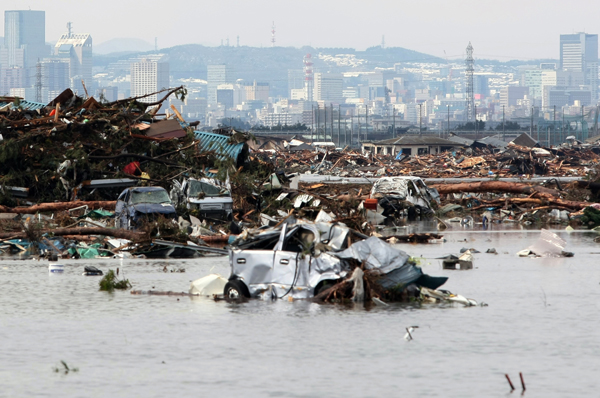
\includegraphics[width=\textwidth,height=0.8\textwidth]{Tsunami.jpg}
      \end{minipage}
      \hfill
      \begin{minipage}[t]{0.48\textwidth}
        \centering
        
        \caption*{Fukushima nuclear disaster. In its immediate aftermath, evacuees reached 7.6\% of Fukushima's population.}
        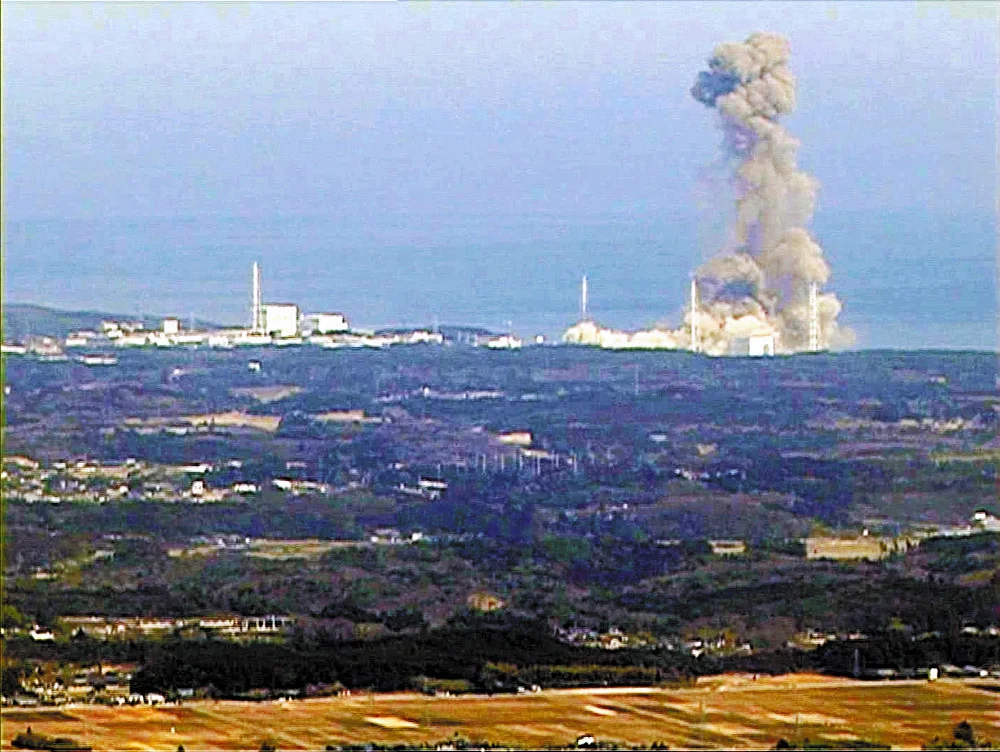
\includegraphics[width=\textwidth,height=0.8\textwidth]{Nuclear_explosion.png}
      \end{minipage}

    \end{figure}
    
    \end{minipage}
\end{frame}

%%%%%%%%%%%%%%%%%%%%%%%%%%%%%%%%%%%%%%%%%%%%%
\begin{frame}{Great East Japan Earthquake (March 2011)}
    \begin{minipage}{1.00\textwidth}

    \raggedright % 全体を左寄せにする
    \begin{flushleft}
\begin{table}[h!]
\vspace{-1.0cm} % 上部の空白を詰める
\raggedright
The magnitude 9.0 mainshock caused massive tsunami waves. The tsunami caused a total power failure at Fukushima Daiichi, leading to a reactor meltdown and hydrogen explosion.
\vspace{-0.12cm} % 上部の空白を詰める
  \label{table:disaster_situation}
  \begin{minipage}[c]{0.4\textwidth}
    \includegraphics[width=\textwidth,height=1.10\textwidth]{epicenter.jpeg}
  \end{minipage}
  \begin{minipage}[c]{0.51\textwidth}
    \raggedright
    \scalebox{0.8}{
    \begin{tabular}{|c|c|c|c|}
    \hline
    & \multicolumn{1}{c|}{Iwate} & \multicolumn{1}{c|}{Miyagi} & \multicolumn{1}{c|}{Fukushima} \\
    \hline
    Population & 1,330,147 & 2,348,165 & 2,029,064 \\
    Deceased & 4,675 & 9,544 & 1,614 \\
    Missing & 1,110 & 1,213 & 196 \\
    Fully destroyed houses & 20,185 & 83,932 & 20,136 \\
    Partially destroyed houses & 4,562 & 138,721 & 65,093 \\
    \hline
    \end{tabular}
    }
  \end{minipage}
  
  \vspace{-1.95cm} % キャプションとの間隔を調整
  \raggedleft{\small Table 1: Direct Damage Status of the Three Most Affected Prefectures}
\end{table}
\end{flushleft}
    \end{minipage}
    
\end{frame}

%%%%%%%%%%%%%%%%%%%%%%%%%%%%%%%%%%%%%%%

\begin{frame}[label=evacuees_main]
\frametitle{Number of Evacuees by Prefecture (2011-2021)}
    \vspace{-0.7cm}
    \begin{columns}[T, onlytextwidth]
        % Table on the left
        \begin{column}{0.5\textwidth}
            \begin{table}[ht]
                \scriptsize
                \setlength{\tabcolsep}{4pt}
                \renewcommand{\arraystretch}{1.0}
                \begin{tabular}{@{}lS[table-format=6.0]S[table-format=6.0]S[table-format=6.0]S[table-format=6.0]S[table-format=6.0]@{}}
                \toprule
                Prefecture & {2011} & {2013} & {2015} & {2017} & {2021} \\
                \midrule
                Iwate & 43953 & 35925 & 23525 & 9204 & 771 \\
                Miyagi & 122557 & 92290 & 50206 & 10548 & 1273 \\
                Fukushima & 95200 & 87712 & 57775 & 18024 & 6777 \\
                Other pref. & 70981 & 58161 & 50494 & 39660 & 30061 \\
                \midrule
                Total & 332691 & 274088 & 182000 & 77436 & 38882 \\
                \bottomrule
                \end{tabular}
                \caption{Number of Evacuees by Prefecture}
                \label{tab:evacuees}
            \end{table}
        \end{column}
        
        % Figure on the right (placeholder)
        \begin{column}{0.485\textwidth}
            \begin{figure}[ht]
                \centering
                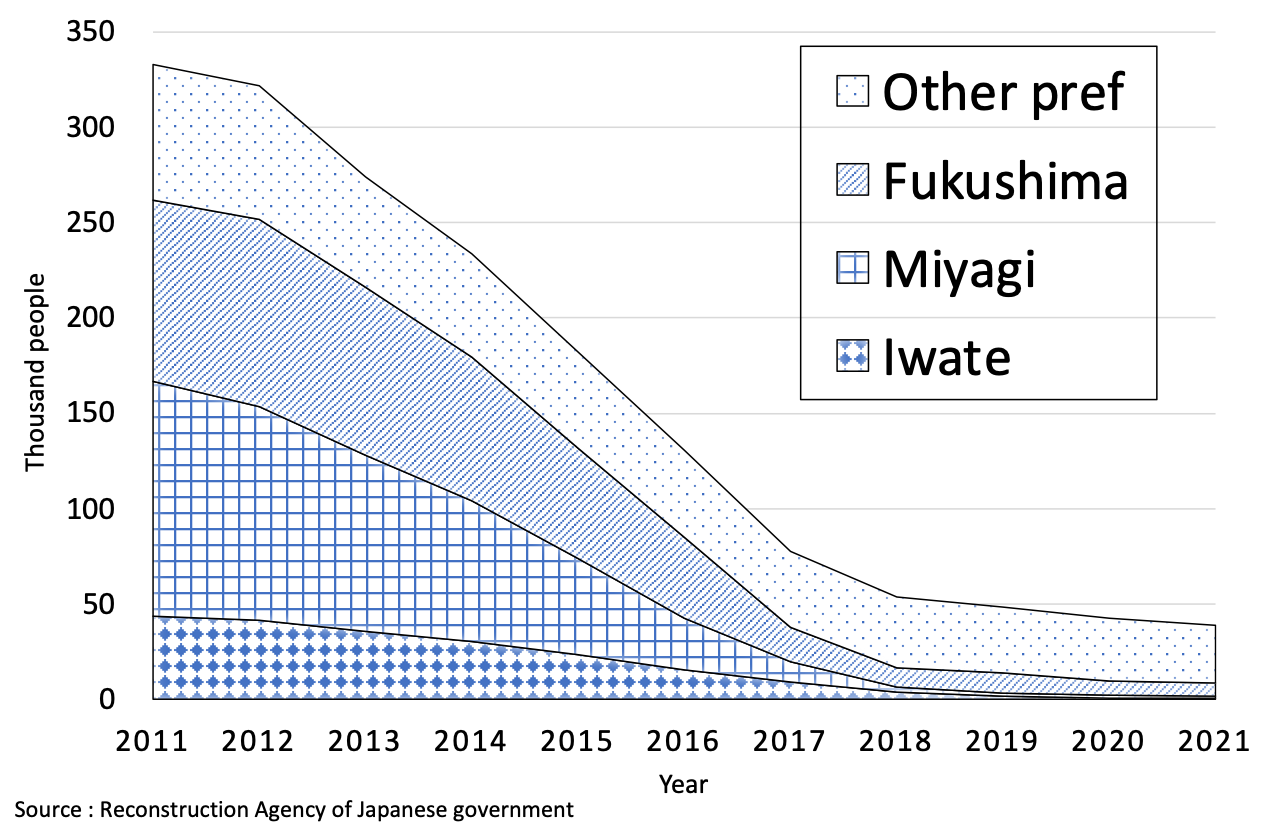
\includegraphics[width=\textwidth]{evacuation.png}
                \caption{Trend of Evacuees by Prefecture}
                \label{fig:evacuees_trend}
            \end{figure}
        \end{column}
    \end{columns}
    


% Explanation text at the bottom of the slide
\begin{column}{0.49\textwidth}
    \raggedright
    \vspace{-2.5cm}
    \hspace{-1.1cm}
    \small{
        \begin{itemize}

            \item Longer displacement in Fukushima
            \item Prolonged evacuation and youth outflow
            \item Significant impact on local labor markets
            \item Tsunami destroyed coastal jobs; affected workforce: Iwate 19.2\%, Miyagi 51.4\%, Fukushima 25.8\%
        \end{itemize}
    }
\end{column}



\vspace{-0.5cm}



\end{frame}

%%%%%%%%%%%%%%%%%%%%%%%%%%%%%

\begin{frame}[label=gender_income_gap]
\frametitle{Significant Wage Gap Between Regular and Non-Regular Workers in Japan (2022)}
\begin{table}[ht]
\centering
\begin{tabular}{lc}
\toprule
Employment Type & Average Annual Income (\$) \\
\midrule
Regular Employment & 40,846 \\
Non-Regular Employment & 23,538 \\
\bottomrule
\multicolumn{2}{r}{\footnotesize Note: Exchange rate \$1 = ¥130} \\
\end{tabular}
\caption{Average Annual Income by Employment Type}
\label{tab:average_income}
\end{table}
\begin{itemize}
\item Non-regular workers are more vulnerable to job termination, receive lower wages, and have fewer opportunities for skill development compared to regular employees.
\end{itemize}
\gendergaplinks
\end{frame}

%%%%%%%%%%%%%%%%%%%%%%%%%%%
%福島のEmployment type 割合
%%%%%%%%%%%%%%%%%%%%%%%%%%%

\begin{frame}[label=proportion_of_employment_type]
\frametitle{Employment Types by Gender - Fukushima Pref. (2010)}

The pre-existing gender disparities in employment types in Fukushima Prefecture before the 2011 disaster. Men were predominantly regular employees (62.7\%), while women were more likely to be in non-regular positions, particularly part-time work (36.8\%).

\vspace{0.5em} % Slight space added

\centering % Center the bar graph

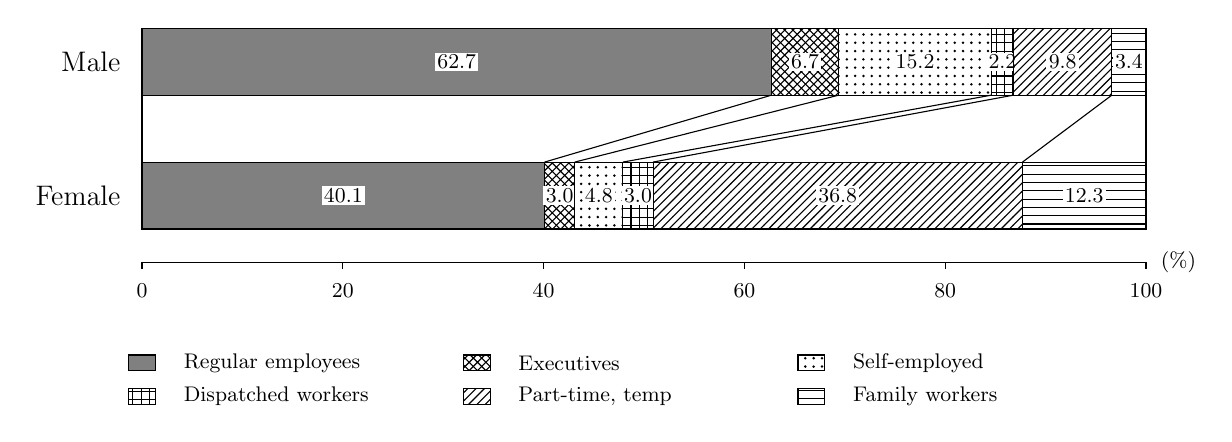
\begin{tikzpicture}[scale=0.85, transform shape]
    % Define colors
    \definecolor{color1}{RGB}{128,128,128}   % Regular employees
    \definecolor{color2}{RGB}{200,200,200}   % Executives
    \definecolor{color3}{RGB}{220,220,220}   % Self-employed
    \definecolor{color4}{RGB}{180,180,180}   % Dispatched workers
    \definecolor{color5}{RGB}{100,100,100}   % Part-time workers
    \definecolor{color6}{RGB}{60,60,60}      % Family workers

    % Bar length multiplier
    \def\barlength{15}

    % Male bar
    \draw[fill=color1] (0,10) rectangle (9.405,11) 
        node[pos=0.5, text=black, fill=white, inner sep=1pt] {\small 62.7};
    \draw[fill=color2, pattern=crosshatch] (9.405,10) rectangle (10.41,11) 
        node[pos=0.5, text=black, fill=white, inner sep=1pt] {\small 6.7};
    \draw[fill=color3, pattern=dots] (10.41,10) rectangle (12.69,11) 
        node[pos=0.5, text=black, fill=white, inner sep=1pt] {\small 15.2};
    \draw[fill=color4, pattern=grid] (12.69,10) rectangle (13.02,11) 
        node[pos=0.5, text=black, fill=white, inner sep=1pt] {\small 2.2};
    \draw[fill=color5, pattern=north east lines] (13.02,10) rectangle (14.49,11) 
        node[pos=0.5, text=black, fill=white, inner sep=1pt] {\small 9.8};
    \draw[fill=color6, pattern=horizontal lines] (14.49,10) rectangle (\barlength,11) 
        node[pos=0.5, text=black, fill=white, inner sep=1pt] {\small 3.4};

    % Female bar
    \draw[fill=color1] (0,8) rectangle (6.015,9) 
        node[pos=0.5, text=black, fill=white, inner sep=1pt] {\small 40.1};
    \draw[fill=color2, pattern=crosshatch] (6.015,8) rectangle (6.465,9) 
        node[pos=0.5, text=black, fill=white, inner sep=1pt] {\small 3.0};
    \draw[fill=color3, pattern=dots] (6.465,8) rectangle (7.185,9) 
        node[pos=0.5, text=black, fill=white, inner sep=1pt] {\small 4.8};
    \draw[fill=color4, pattern=grid] (7.185,8) rectangle (7.635,9) 
        node[pos=0.5, text=black, fill=white, inner sep=1pt] {\small 3.0};
    \draw[fill=color5, pattern=north east lines] (7.635,8) rectangle (13.155,9) 
        node[pos=0.5, text=black, fill=white, inner sep=1pt] {\small 36.8};
    \draw[fill=color6, pattern=horizontal lines] (13.155,8) rectangle (\barlength,9) 
        node[pos=0.5, text=black, fill=white, inner sep=1pt] {\small 12.3};

    % Auxiliary lines
    \draw[black, thin] (0,10) -- (0,9);
    \draw[black, thin] (9.405,10) -- (6.015,9);
    \draw[black, thin] (10.41,10) -- (6.465,9);
    \draw[black, thin] (12.69,10) -- (7.185,9);
    \draw[black, thin] (13.02,10) -- (7.635,9);
    \draw[black, thin] (14.49,10) -- (13.155,9);
    \draw[black, thin] (\barlength,10) -- (\barlength,9);

    % Labels
    \node[anchor=east] at (-0.2,10.5) {\large Male};
    \node[anchor=east] at (-0.2,8.5) {\large Female};

    % X-axis
    \draw (0,7.5) -- (\barlength,7.5);
    \foreach \x in {0,20,40,60,80,100} {
        \pgfmathsetmacro{\pos}{\x * \barlength / 100}
        \draw (\pos,7.5) -- (\pos,7.4) 
            node[anchor=north] at (\pos,7.3) {\small \x};
    }
    \node[anchor=west, font=\small] at (\barlength+0.1,7.5) {(\%)};

    % Adjusted Legend: shifted up and left by approximately 5 characters (~2.5cm)
    \begin{scope}[xshift=-2.5cm]
        % First Row
        \node[anchor=center, fill=color1, minimum width=0.4cm, minimum height=0.2cm, draw] at (2.5,6) {};
        \node[anchor=west] at (3,6) {\small Regular employees};
        
        \node[anchor=center, fill=color2, pattern=crosshatch, minimum width=0.4cm, minimum height=0.2cm, draw] at (7.5,6) {};
        \node[anchor=west] at (8,6) {\small Executives};
        
        \node[anchor=center, fill=color3, pattern=dots, minimum width=0.4cm, minimum height=0.2cm, draw] at (12.5,6) {};
        \node[anchor=west] at (13,6) {\small Self-employed};
        
        % Second Row
        \node[anchor=center, fill=color4, pattern=grid, minimum width=0.4cm, minimum height=0.2cm, draw] at (2.5,5.5) {};
        \node[anchor=west] at (3,5.5) {\small Dispatched workers};
        
        \node[anchor=center, fill=color5, pattern=north east lines, minimum width=0.4cm, minimum height=0.2cm, draw] at (7.5,5.5) {};
        \node[anchor=west] at (8,5.5) {\small Part-time, temp};
        
        \node[anchor=center, fill=color6, pattern=horizontal lines, minimum width=0.4cm, minimum height=0.2cm, draw] at (12.5,5.5) {};
        \node[anchor=west] at (13,5.5) {\small Family workers};
    \end{scope}
\end{tikzpicture}

\vspace{0.5em} % Space between the bar graph and legend

% \links placed inside the frame
\employmenttypelinks

\end{frame}

%%%%%%%%%%%%%%%%%%%%%%%%%%%%%%%%%%%

\begin{frame}[label=short_term_unemployment]
\frametitle{Short-term changes
in unemployment insurance recipients in Fukushima}

    \centering
    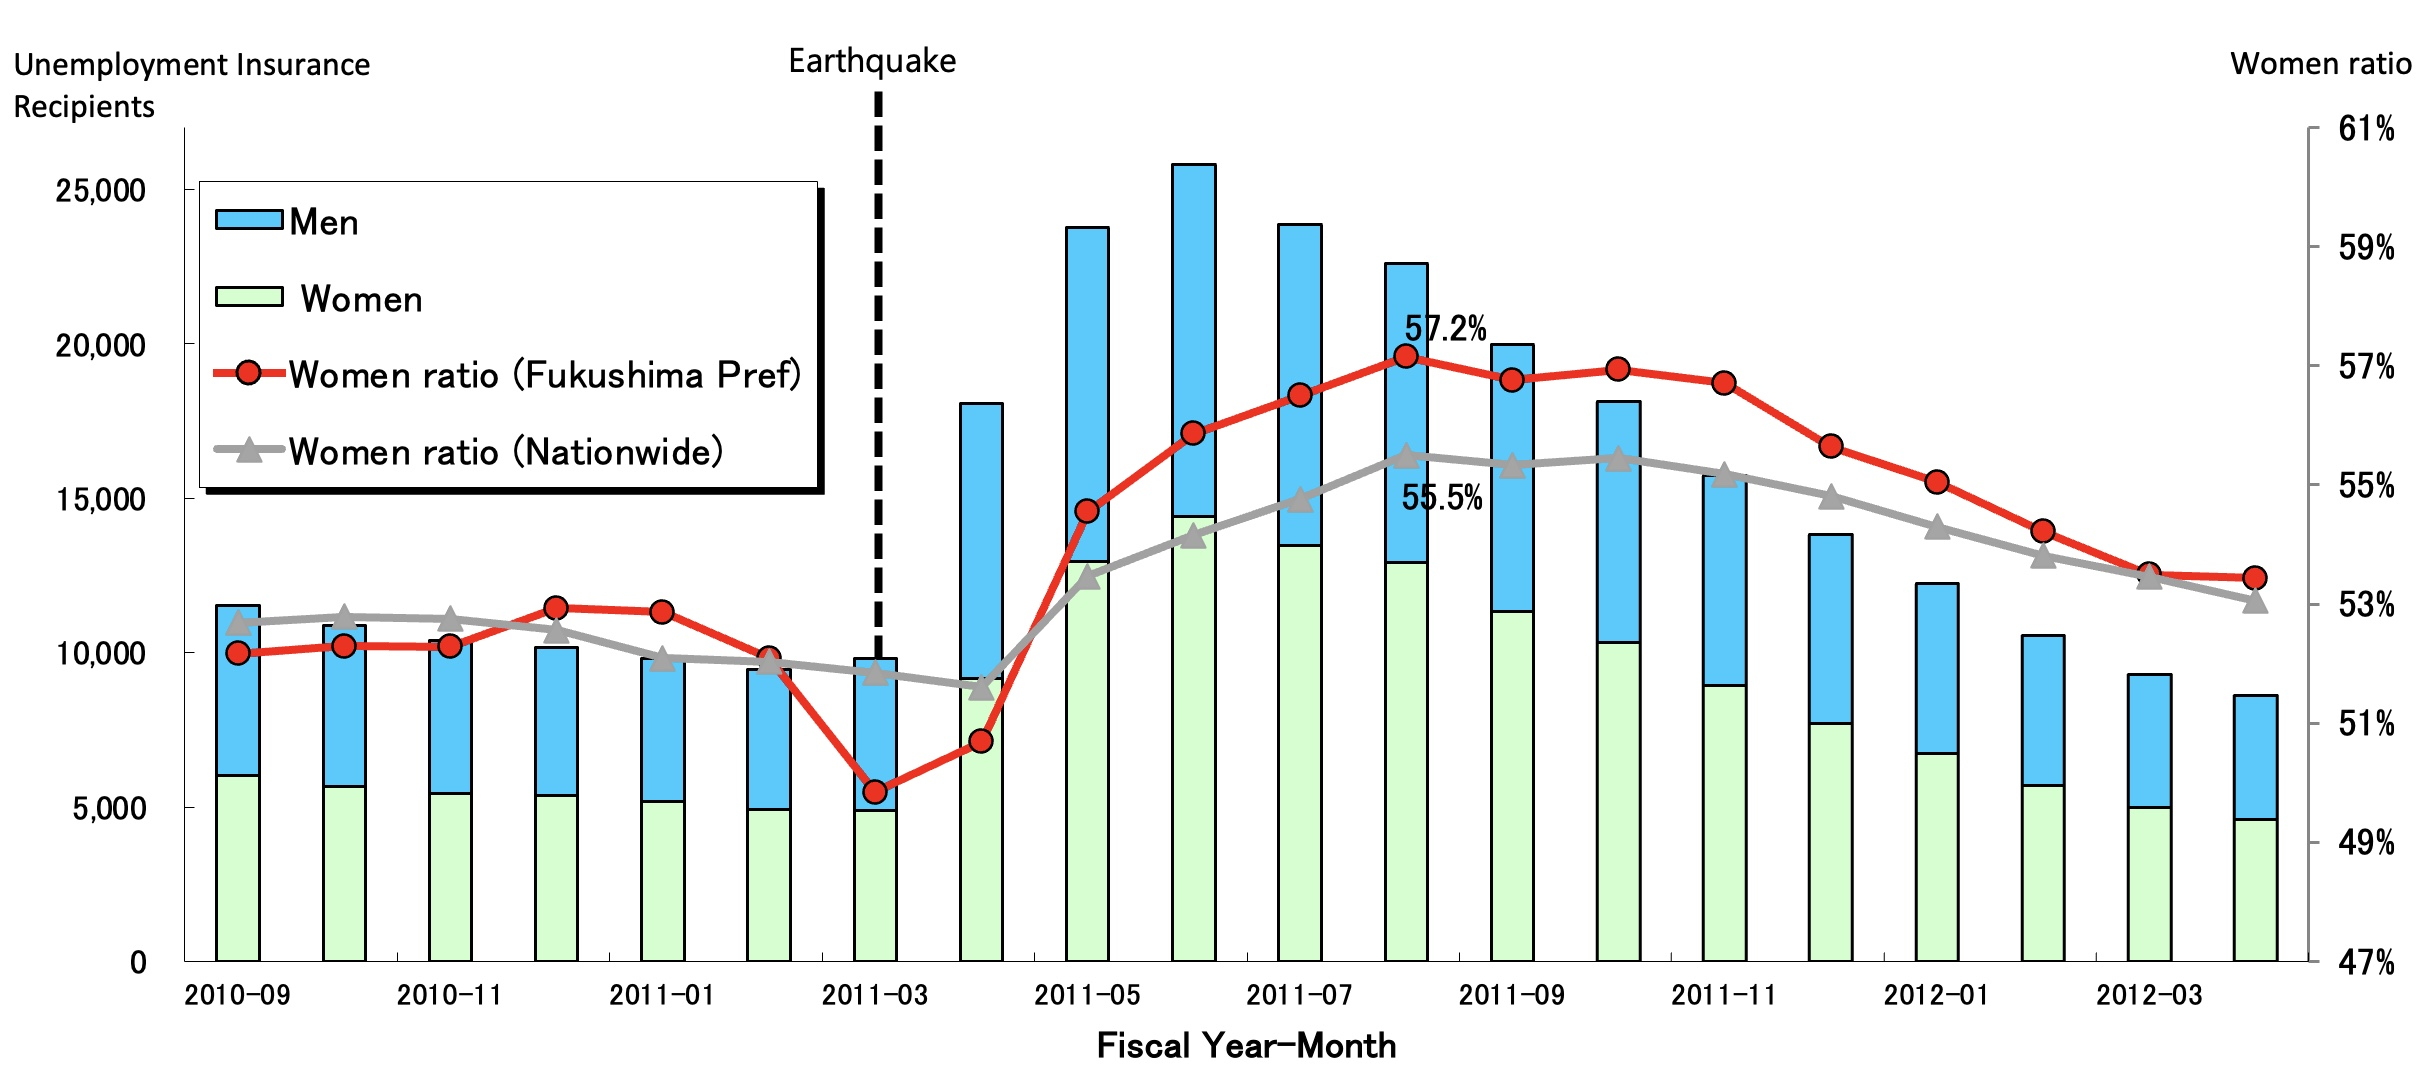
\includegraphics[width=0.8\textwidth]{Number of Actual unemployment insurance recipants (short-term).jpeg}
    \vspace{0.5cm}

\begin{minipage}{0.8\textwidth}
    {\small
        {The ratio of women unemployment insurance recipients in Fukushima increased sharply after the disaster, surpassing the national average.}
    }
\end{minipage}

\unemploymentinsurancelinks

\end{frame}
%%%%%%%%%%%%%%%%%%%%%%%%%%%%%%%%


%%%%%%%%%%%%%%%%%%%%%%%%%%%%%%%%
\section{Motivation \& Research Questions}
%%%%%%%%%%%%%%%%%%%%%%%%%%%%%%%%

\begin{frame}{Motivation \& Research Questions}
    \begin{center}

\vspace{-0.30cm} 
    
        \Large\textbf{Does the Gender Income Gap Expand in Areas Affected by a Disaster? Evidence from the Great East Japan Earthquake}
        \vspace{-0.3cm}

    \end{center}
    \vspace{0.2cm}
    
    \begin{columns}[T]
        \begin{column}{0.5\textwidth}
            \textbf{Motivation:}
            \begin{itemize}\small
                \item Intersection of gender inequality and disaster impacts
                \item Addressing research gap in dynamic relationship between disasters and gender
                \item Urgent need to understand disaster-induced economic disparities
                \item Unraveling complex mechanisms using multiple datasets
                \item Informing policy for effective post-disaster recovery
            \end{itemize}
        \end{column}
        
        \begin{column}{0.5\textwidth}
            \textbf{Research Questions:}
            \begin{itemize}\small
                \item Does the gender income gap expand in disaster-affected areas?
                \item How do disaster impacts differ by:
                    \begin{itemize}\footnotesize
                        \item Short-term vs. long-term effects
                        \item Gender
                        \item Employment status
                        \item Industry
                    \end{itemize}
                \item What mechanisms drive these differential impacts?
            \end{itemize}
        \end{column}
    \end{columns}
\end{frame}

%%%%%%%%%%%%%%%%%%%%%%%%%%%%%%%%



%%%%%%%%%%%%%%%%%%%%%%%%%%%%%%%%
\section{Literature Review}
%%%%%%%%%%%%%%%%%%%%%%%%%%%%%%%%

\begin{frame}[label=literature_review2]
\frametitle{Literature Review: Theoretical Perspectives on Gender Disparities}

    \begin{table}[ht]
        \centering
        \begin{tabular}{>{\raggedright}p{3cm} p{10cm}}
            \hline
            \textbf{Theory} & \textbf{Key Insights} \\
            \hline

\addlinespace
            
            Risk Adjustment Hypothesis & Women are more vulnerable to labor market shocks during disasters, leading to higher unemployment rates and income declines. (\citealt{Kim2014ARetention}; \citealt{Groger2016InternalTyphoon})\\

\addlinespace
            
            Shock Coping Strategy & Women may increase labor supply post-disaster as a coping mechanism, potentially enhancing income and employment opportunities. (\citealt{Porcelli2019TheItaly}; \citealt{Deryugina2018TheReturns}; \citealt{Canessa2021WomensShocks})\\
            \hline
        \end{tabular}

        \label{tab:theoretical_perspectives}
    \end{table}
    
    \vspace{0.1cm}
    
    This study aims to bridge the gap in existing literature by examining both short-term and long-term effects of the March 2011 disaster on gender disparities in income, addressing the contradictory findings of previous research.

\literaturelinks

\end{frame}

%%%%%%%%%%%%%%%%%%%%%%%%%%%%%%%%%%%


\begin{frame}[label=literature_review1]
\frametitle{Literature review: Time Series Analysis of Disaster Economic Impacts}

    \begin{minipage}[c]{0.4\linewidth}
        \small

        \vspace{-2.3cm}
        
Short-term and long-term effects of disasters (e.g., \citet{Deryugina2018TheReturns} ): 
\begin{itemize}
    \item Phase 1: Immediate and severe negative economic impact on disaster-affected areas.
    \item Phase 2: Recovery driven by reconstruction boom, offsetting initial negative impact((\ding{172}$<$\ding{173}) ).
    \item Phase 3: Return to pre-disaster trend (Returning to the steady state).
\end{itemize}


This study aims to capture the long-term economic impact over several years following the disaster.

        
        \vspace{-2.1cm}
        

    \end{minipage}\hspace{0.5cm}
    \begin{minipage}{0.3\linewidth}
        \medskip
        \begin{figure}[h]
            \centering
            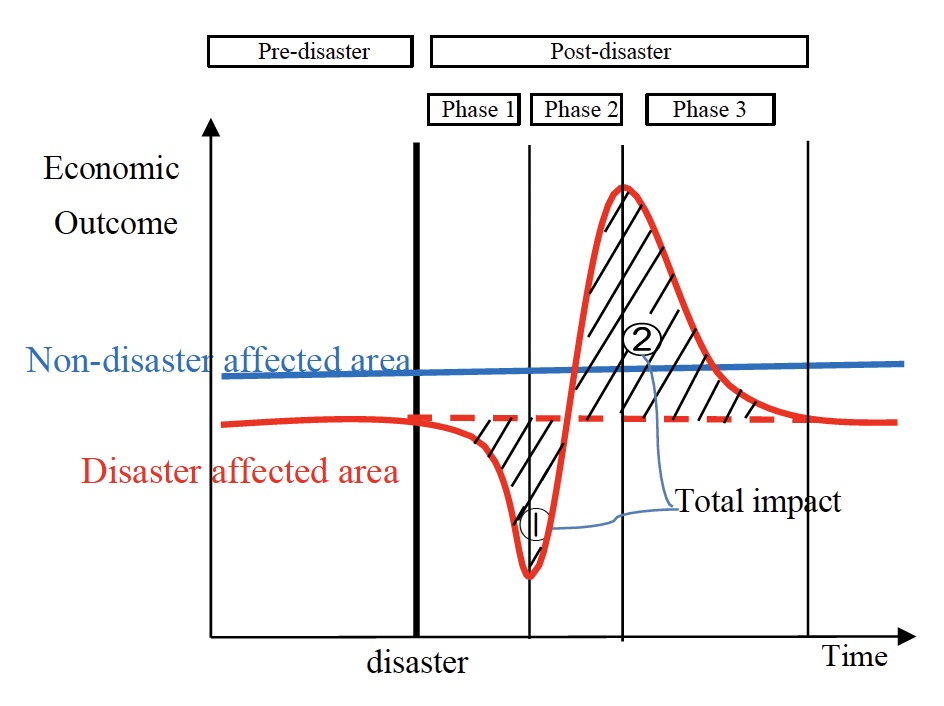
\includegraphics[height=.8\textheight]{conceptual_image.jpeg}
        \end{figure}
    \end{minipage}

\longtermimpactlinks

\end{frame}

%%%%%%%%%%%%%%%%%%%%%%%%%%%%%%%%%%%
\section{Methods}
%%%%%%%%%%%%%%%%%%%%%%%%%%%%%%%%%%%


%---------------------------------------
% Slide: Data
%---------------------------------------

\begin{frame}[label=data]
\frametitle{Data}

    \vspace{-0.2cm}
  \begin{figure}
    \centering
    \includegraphics[width=0.93\textwidth]{list_of_individual_data2.png}

  \end{figure}

Note: The sample excludes metropolitan areas (Tokyo, Kanagawa, Saitama, Chiba, Osaka, Kyoto, Hyogo, and Aichi) and is restricted to individuals aged 15 and above.

\datalinks


\end{frame}

%%%%%%%%%%%%%%%%%%%%%%%%%%%%%%%%%%%%%

\begin{frame}[label=employment_categories]
\frametitle{}

\begin{table}[htbp]
\centering
\caption{Employment Status Categories in the Population Census and Study Classification}
\resizebox{0.8\textwidth}{!}{
\small
\begin{tabular}{>{\raggedright\arraybackslash}p{0.3\textwidth}>{\raggedright\arraybackslash}p{0.4\textwidth}>{\raggedright\arraybackslash}p{0.2\textwidth}}
\toprule
\textbf{Census Category} & \textbf{Definition} & \textbf{Study Classification} \\
\midrule
Regular employees & Regular employee has an indefinite employment contract with the employer. & \multirow{3}{*}{Regular workers} \\
\cmidrule{1-2}
Executives & Directors of a company or a corporation including managing directors. & \\
\cmidrule{1-2}
Self-employed & Persons who ran a business with or without employees. & \\
\midrule
Dispatched workers from temporary labour agency & Dispatched worker from temporary labour agency based on relevant low. & \multirow{3}{*}{Non-regular workers} \\
\cmidrule{1-2}
Part-time/temporary employees and others & "Part-time worker", "Arbeit (temporary worker)" and "Contract employee or entrusted employee". & \\
\cmidrule{1-2}
Family workers & Persons who worked in a business operated by a member of the household in which they lived. & \\
\bottomrule
\end{tabular}
}
\label{tab:employment_status}
\begin{flushleft}
\footnotesize
%\textit{Note}: This table shows the original categories from the Population Census and how I classified in this study. "Self-employed" combines both categories of self-employed (with and without employees) from the census. "Persons doing home handicraft" from the census are included in the "Family workers" category.\\
%\textit{Source}: Adapted from Statistics Bureau of Japan, Population Census webpage: \url{https://www.stat.go.jp/english/data/kokusei/index.html}
\end{flushleft}
\end{table}

\vspace{-0.2cm}

\workersinks

\end{frame}

%%%%%%%%%%%%%%%%%%%%%%%%%%%%%%%%
%%%%%%%%%%%%%%%%%%%%%%%%%%%%%%%%
\begin{frame}{Methodology and Empirical Strategy: Descriptive statistics and Basic DID}
    \begin{itemize}
    \item  Using descriptive statistics on JGSS and a basic DiD analysis on Population census dividing samples into male and female groups and estimates the disaster's impact on various outcome variables of concern.

\begin{equation}
Y_{ipt} = \alpha + \beta_1 \text{Post}_t + \beta_2 (\text{Fukushima}_p \cdot \text{Post}_t) + \gamma X_{ipt} + \delta_p + \epsilon_{ipgt}
\end{equation}

\end{itemize}


$Y_{ipt}$ denotes the concerned outcome variable such as employment type (e.g., non-regular worker or not) for individual $i$ in prefecture $p$ at year $t$. $\text{Fukushima}_p$ is a binary indicator for Fukushima Prefecture. $\text{Post}_t$ is a binary indicator for the post-disaster year (2015), with the pre-disaster year being 2010. The coefficient $\beta_2$ represents the DID estimate, capturing the disaster's impact on the probability of regular employment in Fukushima. $X_{ipt}$ are individual control variables that include age group, marital status, residence duration, relation ship with head, residence type and household size. $\delta_p$ represents prefecture fixed effects.



\end{frame}
%%%%%%%%%%%%%%%%%%%%%%%%%%%%%%%%


%%%%%%%%%%%%%%%%%%%%%%%%%%%%%%%%
\section{Results}
%%%%%%%%%%%%%%%%%%%%%%%%%%%%%%%%

\begin{frame}[label=income_band_main]
\frametitle{Income Bands by Gender: Pre- (2000-2010) vs Post-Disaster (2012-2018) Analysis (JGSS)}
    \vspace{-0.7cm}
    \begin{columns}[T, onlytextwidth]
        % テーブルを左側に配置
        \begin{column}{0.5\textwidth}
            \begin{table}[ht]
                \scriptsize
                \setlength{\tabcolsep}{4pt}
                \renewcommand{\arraystretch}{1.0}
                \begin{tabular}{lccccc}
                    \toprule
                    \multirow{2}{*}{Gender} & \multirow{2}{*}{Prefecture} & \multicolumn{2}{c}{Mean Income} & \multirow{2}{*}{Change (\%)} & \multirow{2}{*}{P-value} \\
                    & & Pre & Post & & \\
                    \midrule
                    \multirow{2}{*}{Male} 
                        & Affected & \textcolor{blue}{7.967} & \textcolor{red}{7.835} & -1.67 & 0.654 \\
                        & Unaffected & \textcolor{blue}{8.660} & \textcolor{red}{8.300} & \quad -4.16*** & 0.000 \\
                    \midrule
                    \multirow{2}{*}{Female} 
                        & Affected & \textcolor{blue}{4.721} & \textcolor{red}{5.183} & +9.79* & 0.065 \\
                        & Unaffected & \textcolor{blue}{4.995} & \textcolor{red}{5.087} & +1.83 & 0.143 \\
                    \bottomrule
                    \multicolumn{6}{@{}p{\textwidth}}{\footnotesize $*p<0.1$, $**p<0.05$, $***p<0.01$} \\
                \end{tabular}
                \caption{Mean Annual Income from Main Job: Pre/Post-Disaster Period (Income bands, N=20,119)}
                \label{tab:income}
            \end{table}
        \end{column}
        
        % 図を右側に配置
        \begin{column}{0.485\textwidth}
            \begin{figure}[ht]
                \centering
                \includegraphics[width=\textwidth]{Kernel density graphs of respondent’s annual income from main job.png}
                \caption{Kernel Density of Annual Income from Main Job (Income bands, N=20,119)}
                \label{fig:kde_income}
            \end{figure}
        \end{column}
    \end{columns}
    
    % 説明文をスライドの下部に配置
    \begin{column}{0.49\textwidth}
            \raggedright
    
    \vspace{-2.5cm}
    \hspace{-1.1cm}
\large {\qquad \ \ Women in affected prefectures experienced the largest income increase (+9.79\%) post-disaster (a rightward shift (increase) in average income bands when comparing pre- and post-disaster periods).}
    \end{column}
\vspace{-0.7cm}
\incomebandlinks
\end{frame}

%%%%%%%%%%%%%%%%%%%%%%%%%%%%%%%%
%\cmidrule(lr){2-4}\cmidrule(lr){5-7}
%%%%%%%%%%%%%%%%%%%%%%%%%%%%%%%%%%%

\begin{frame}[label=regular_status]

The DID analysis shows a significant positive impact on regular worker status for both genders in Fukushima, with a larger effect for males. The fully specified model indicates a 1.6 percentage point increase for males and a 0.5 percentage point increase for females.

\begin{table}[htbp]
\centering
\caption{OLS Estimates of Disaster Impact on Regular Worker Status}

\vspace{-0.2cm}

\scalefont{0.55}

\begin{tabular}{@{}l*{6}{c}@{}}
          &\multicolumn{3}{c}{Male}                                &\multicolumn{3}{c}{Female}                              \\\cmidrule(lr){2-4}\cmidrule(lr){5-7}
          &\multicolumn{1}{c}{(1)}         &\multicolumn{1}{c}{(2)}         &\multicolumn{1}{c}{(3)}         &\multicolumn{1}{c}{(4)}         &\multicolumn{1}{c}{(5)}         &\multicolumn{1}{c}{(6)}         \\
\toprule
Disaster Impact (DID)&    0.010\sym{***}&    0.011\sym{***}&    0.016\sym{***}&    0.005\sym{***}&    0.002         &    0.005\sym{***}\\
          &  (0.002)         &  (0.002)         &  (0.002)         &  (0.001)         &  (0.001)         &  (0.001)         \\
\addlinespace
Post-Disaster Period&   -0.009\sym{***}&    0.013\sym{***}&    0.018\sym{***}&    0.006\sym{***}&    0.016\sym{***}&    0.017\sym{***}\\
          &  (0.002)         &  (0.002)         &  (0.002)         &  (0.001)         &  (0.001)         &  (0.001)         \\
\addlinespace
Married   &                  &    0.253\sym{***}&    0.148\sym{***}&                  &   -0.116\sym{***}&   -0.059\sym{***}\\
          &                  &  (0.005)         &  (0.003)         &                  &  (0.004)         &  (0.004)         \\
\midrule
Age Group &       No         &      Yes         &      Yes         &       No         &      Yes         &      Yes         \\
Residence Duration&       No         &       No         &      Yes         &       No         &       No         &      Yes         \\
Relationship with Head&       No         &       No         &      Yes         &       No         &       No         &      Yes         \\
Residence Type&       No         &       No         &      Yes         &       No         &       No         &      Yes         \\
Household Size&       No         &       No         &      Yes         &       No         &       No         &      Yes         \\
$\textit{N}$&   540474         &   540474         &   540474         &   598422         &   598422         &   598422         \\
$\textit{R}^2$&    0.003         &    0.343         &    0.400         &    0.003         &    0.142         &    0.164         \\
Control Mean&    0.536         &    0.536         &    0.536         &    0.210         &    0.210         &    0.210         \\
\bottomrule
\end{tabular}
\\\\{\linewidth}{\tiny Standard errors clustered at prefecture level in parentheses}\\\\
\\\\{\linewidth}{\tiny $*p<0.1$, $**p<0.05$, $***p<0.01$}\\\\
\\\\{\linewidth}{\tiny \textit{Note}: This table reports OLS estimates of the disaster's impact on regular worker status for males and females under various model specifications. Metropolitan areas (Tokyo, Kanagawa, Saitama, Chiba, Osaka, Kyoto, Hyogo, and Aichi) are excluded, and the sample is restricted to individuals aged 15 and above. The dependent variable is a binary indicator for regular worker status, including individuals categorized as unknown. All models include prefecture fixed effects, with standard errors clustered at the prefecture level. The marital status variable equals 1 for those with a spouse present and 0 for those never married, widowed, or divorced. Control Mean refers to the pre-disaster mean of the dependent variable for the non-Fukushima control group.}
\end{table}

\vspace{-2.0cm}
\regularlinks

\end{frame}

% ----------------------------------------------------
% Placebo: DID analysis with OLS Models (occupation variable excluded)
% Corrected Code with Residence Duration Removed from Results and Updated Variable Labels
% All variables are strings
% ----------------------------------------------------
\begin{frame}[label=regular_placebo]

The placebo test (2000-2005) shows significant negative impacts on regular worker status for both genders, contrasting with the positive effects in the main analysis (2010-2015). This reversal suggests the disaster may have disrupted pre-existing trends.


\vspace{-1.0cm}
\returnbutton{regular_status}{Return}
\vspace{1.2cm}

\begin{table}[htbp]
\centering
\caption{Placebo Test: OLS Estimates of Disaster Impact on Regular Worker Status (2000-2005)}

\vspace{-0.2cm}

\scalefont{0.61}

\begin{tabular}{@{}l*{6}{c}@{}}
          &\multicolumn{3}{c}{Male}                                &\multicolumn{3}{c}{Female}                              \\\cmidrule(lr){2-4}\cmidrule(lr){5-7}
          &\multicolumn{1}{c}{(1)}         &\multicolumn{1}{c}{(2)}         &\multicolumn{1}{c}{(3)}         &\multicolumn{1}{c}{(4)}         &\multicolumn{1}{c}{(5)}         &\multicolumn{1}{c}{(6)}         \\
\toprule
Placebo Disaster Impact (DID)&   -0.009\sym{***}&   -0.007\sym{***}&   -0.009\sym{***}&   -0.005\sym{***}&   -0.009\sym{***}&   -0.009\sym{***}\\
          &  (0.002)         &  (0.002)         &  (0.002)         &  (0.001)         &  (0.001)         &  (0.001)         \\
\addlinespace
Placebo Post-Period&   -0.040\sym{***}&   -0.023\sym{***}&   -0.021\sym{***}&   -0.009\sym{***}&    0.003\sym{**} &    0.000         \\
          &  (0.002)         &  (0.002)         &  (0.002)         &  (0.001)         &  (0.001)         &  (0.001)         \\
\addlinespace
Married   &                  &    0.224\sym{***}&    0.130\sym{***}&                  &   -0.168\sym{***}&   -0.092\sym{***}\\
          &                  &  (0.006)         &  (0.004)         &                  &  (0.006)         &  (0.005)         \\
\midrule
Age Group &       No         &      Yes         &      Yes         &       No         &      Yes         &      Yes         \\
Relationship with Head&       No         &       No         &      Yes         &       No         &       No         &      Yes         \\
Residence Type&       No         &       No         &      Yes         &       No         &       No         &      Yes         \\
Household Size&       No         &       No         &      Yes         &       No         &       No         &      Yes         \\
$\textit{N}$&   550771         &   550771         &   550771         &   606094         &   606094         &   606094         \\
$\textit{R}^2$&    0.006         &    0.383         &    0.400         &    0.003         &    0.214         &    0.224         \\
Control Mean&    0.651         &    0.651         &    0.651         &    0.332         &    0.332         &    0.332         \\
\bottomrule
\end{tabular}
\\\\{\linewidth}{\tiny Standard errors clustered at prefecture level in parentheses}\\\\
\\\\{\linewidth}{\tiny $*p<0.1$, $**p<0.05$, $***p<0.01$}\\\\
\\\\{\linewidth}{\tiny \textit{Note}: This table presents OLS estimates of the placebo disaster impact on regular worker status for both males and females using 2000 and 2005 population census data, excluding metropolitan areas. Residence Duration is not included as it is unavailable in the 2005 data set. The occupation variable is also excluded. All models include prefecture fixed effects, and the error term is clustered at the prefecture level. Control Mean represents the average proportion of regular workers in non-Fukushima prefectures before the placebo disaster period.}
\end{table}


\end{frame}

%%%%%%%%%%%%%%%%%%%%%%%%%%%%%%%%

%\begin{frame}

%The DID analysis on non-regular worker status shows no statistically significant effect for males in the fully specified model. For females, the full model indicates a small but significant decrease (0.2 percentage points) in the probability of being a non-regular worker in Fukushima.

%\begin{table}[htbp]
%\centering
%\caption{OLS Estimates of Disaster Impact on Non-Regular Worker Status}

%\scalefont{0.60}

%\begin{tabular}{@{}l*{6}{c}@{}}
          %&\multicolumn{3}{c}{Male}                                &\multicolumn{3}{c}{Female}                              \\\cmidrule(lr){2-4}\cmidrule(lr){5-7}
          %&\multicolumn{1}{c}{(1)}         &\multicolumn{1}{c}{(2)}         &\multicolumn{1}{c}{(3)}         &\multicolumn{1}{c}{(4)}         &\multicolumn{1}{c}{(5)}         &\multicolumn{1}{c}{(6)}         \\
%\toprule
%Disaster Impact (DID)&   -0.001         &   -0.003\sym{**} &   -0.005\sym{***}&   -0.006\sym{***}&   -0.008\sym{***}&   -0.004\sym{***}\\
          %&  (0.001)         &  (0.001)         &  (0.001)         &  (0.001)         &  (0.001)         &  (0.001)         \\
%\addlinespace
%Post-Disaster Period&    0.003\sym{**} &    0.003\sym{**} &   -0.000         &    0.004\sym{***}&    0.012\sym{***}&    0.000         \\
          %&  (0.001)         &  (0.001)         &  (0.001)         &  (0.001)         &  (0.001)         &  (0.001)         \\
%\addlinespace
%Married   &                  &   -0.050\sym{***}&   -0.088\sym{***}&                  &    0.058\sym{***}&    0.082\sym{***}\\
          %&                  &  (0.001)         &  (0.001)         &                  &  (0.003)         &  (0.003)         \\
%\midrule
%Age       &       No         &      Yes         &      Yes         &       No         &      Yes         &      Yes         \\
%Residence Duration&       No         &       No         &      Yes         &       No         &       No         &      Yes         \\
%Industry  &       No         &       No         &      Yes         &       No         &       No         &      Yes         \\
%$\textit{N}$&  540,474         &  540,474         &  540,474         &  598,422         &  598,422         &  598,422         \\
%$\textit{R}^2$&    0.000         &    0.035         &    0.136         &    0.001         &    0.100         &    0.440         \\
%Control Mean&    0.093         &    0.093         &    0.093         &    0.236         &    0.236         &    0.236         \\
%\bottomrule
%\end{tabular}
%\\\multicolumn{7}{@{}p{\linewidth}}{\footnotesize Standard errors clustered at prefecture level in parentheses}\\
%\multicolumn{7}{@{}p{\linewidth}}{\footnotesize $*p<0.1$, $**p<0.05$, $***p<0.01$}\\

%\end{table}


%\end{frame}

%%%%%%%%%%%%%%%%%%%%%%%%%%%%%%%%%%%

%%%%%%%%%%%%%%%%%%%%%%%%%%%%%%%%
%\cmidrule(lr){2-4}\cmidrule(lr){5-7}
%%%%%%%%%%%%%%%%%%%%%%%%%%%%%%%%%%%

\begin{frame}[label=nonregular_status]

The DID analysis reveals a significant positive impact on non-regular worker status for males in Fukushima, with a 1.0 percentage point increase. In contrast, females show no statistically significant effect.

\begin{table}[htbp]
\centering
\caption{OLS Estimates of Disaster Impact on Non-Regular Worker Status}

\vspace{-0.2cm}

\scalefont{0.53}

\begin{tabular}{@{}l*{6}{c}@{}}
          &\multicolumn{3}{c}{Male}                                &\multicolumn{3}{c}{Female}                              \\\cmidrule(lr){2-4}\cmidrule(lr){5-7}
          &\multicolumn{1}{c}{(1)}         &\multicolumn{1}{c}{(2)}         &\multicolumn{1}{c}{(3)}         &\multicolumn{1}{c}{(4)}         &\multicolumn{1}{c}{(5)}         &\multicolumn{1}{c}{(6)}         \\
\toprule
Disaster Impact (DID)&    0.012\sym{***}&    0.010\sym{***}&    0.010\sym{***}&    0.000         &   -0.002\sym{**} &    0.000         \\
          &  (0.001)         &  (0.001)         &  (0.002)         &  (0.001)         &  (0.001)         &  (0.001)         \\
\addlinespace
Post-Disaster Period&    0.004\sym{**} &    0.005\sym{***}&    0.003\sym{**} &    0.005\sym{***}&    0.013\sym{***}&    0.016\sym{***}\\
          &  (0.001)         &  (0.001)         &  (0.001)         &  (0.001)         &  (0.001)         &  (0.001)         \\
\addlinespace
Married   &                  &   -0.062\sym{***}&   -0.031\sym{***}&                  &    0.054\sym{***}&    0.013\sym{***}\\
          &                  &  (0.002)         &  (0.002)         &                  &  (0.003)         &  (0.004)         \\
\midrule
Age Group &       No         &      Yes         &      Yes         &       No         &      Yes         &      Yes         \\
Residence Duration&       No         &       No         &      Yes         &       No         &       No         &      Yes         \\
Relationship with Head&       No         &       No         &      Yes         &       No         &       No         &      Yes         \\
Residence Type&       No         &       No         &      Yes         &       No         &       No         &      Yes         \\
Household Size&       No         &       No         &      Yes         &       No         &       No         &      Yes         \\
$\textit{N}$&   540474         &   540474         &   540474         &   598422         &   598422         &   598422         \\
$\textit{R}^2$&    0.001         &    0.037         &    0.047         &    0.001         &    0.101         &    0.109         \\
Control Mean&    0.108         &    0.108         &    0.108         &    0.245         &    0.245         &    0.245         \\
\bottomrule
\end{tabular}
\\\\{\linewidth}{\tiny Standard errors clustered at prefecture level in parentheses}\\\\
\\\\{\linewidth}{\tiny $*p<0.1$, $**p<0.05$, $***p<0.01$}\\\\
\\\\{\linewidth}{\tiny \textit{Note}: This table reports OLS estimates of the disaster's impact on non-regular worker status for males and females under various model specifications. Metropolitan areas (Tokyo, Kanagawa, Saitama, Chiba, Osaka, Kyoto, Hyogo, and Aichi) are excluded, and the sample is restricted to individuals aged 15 and above. The dependent variable is a binary indicator for non-regular worker status, including individuals categorized as unknown. All models include prefecture fixed effects, with standard errors clustered at the prefecture level. The marital status variable equals 1 for those with a spouse present and 0 for those never married, widowed, or divorced. Control Mean refers to the pre-disaster mean of the dependent variable for the non-Fukushima control group.}
\end{table}

\vspace{-2.2cm}
\nonregularlinks


\end{frame}
%%%%%%%%%%%%%%%%%%%%%%%%%%%%%%%%
%\cmidrule(lr){2-4}\cmidrule(lr){5-7}
%%%%%%%%%%%%%%%%%%%%%%%%%%%%%%%%%%%





%%%%%%%%%%%%%%%%%%%%%%%%%%%%%%%%%%%%%%%%%%

%\begin{frame}

%The placebo test (2000-2005) reveals coefficients opposite to the main DID results: positive for males and negative for females. This suggests the disaster may have had a reversal effect on pre-existing trends in regular worker status.


%\begin{table}[htbp]

%\centering

%\scalefont{0.62}

%\caption{Placebo Test: OLS Estimates of Disaster Impact on Regular Worker Status (2000-2005)}



%\begin{tabular}{@{}l*{6}{c}@{}}
          %&\multicolumn{3}{c}{Male}                                &\multicolumn{3}{c}{Female}                              \\\cmidrule(lr){2-4}\cmidrule(lr){5-7}
          %&\multicolumn{1}{c}{(1)}         &\multicolumn{1}{c}{(2)}         &\multicolumn{1}{c}{(3)}         &\multicolumn{1}{c}{(4)}         &\multicolumn{1}{c}{(5)}         &\multicolumn{1}{c}{(6)}         \\
%\toprule
%Placebo Disaster Impact (DID)&    0.005\sym{***}&    0.003\sym{***}&    0.003\sym{***}&   -0.011\sym{***}&   -0.011\sym{***}&   -0.007\sym{***}\\
          %&  (0.001)         &  (0.001)         &  (0.001)         &  (0.002)         &  (0.002)         &  (0.002)         \\
%\addlinespace
%Placebo Post-Period&   -0.014\sym{***}&   -0.012\sym{***}&   -0.012\sym{***}&   -0.007\sym{***}&   -0.005\sym{**} &   -0.008\sym{***}\\
          %&  (0.001)         &  (0.001)         &  (0.001)         &  (0.002)         &  (0.002)         &  (0.002)         \\
%\addlinespace
%Married   &                  &    0.071\sym{***}&    0.070\sym{***}&                  &   -0.185\sym{***}&   -0.158\sym{***}\\
          %&                  &  (0.002)         &  (0.002)         &                  &  (0.005)         &  (0.004)         \\
%\midrule
%Age       &       No         &      Yes         &      Yes         &       No         &      Yes         &      Yes         \\
%Industry  &       No         &       No         &      Yes         &       No         &       No         &      Yes         \\
%$\textit{N}$&  380,481         &  380,481         &  380,481         &  283,151         &  283,151         &  283,151         \\
%$\textit{R}^2$&    0.002         &    0.066         &    0.070         &    0.003         &    0.089         &    0.153         \\
%Control Mean&    0.921         &    0.921         &    0.921         &    0.704         &    0.704         &    0.704         \\
%\bottomrule
%\end{tabular}
%\\
%\multicolumn{7}{@{}p{\linewidth}}{\footnotesize Standard errors clustered at prefecture level in parentheses}\\
%\multicolumn{7}{@{}p{\linewidth}}{\footnotesize $*p<0.1$, $**p<0.05$, $***p<0.01$}\\

%\end{table}

%\end{frame}


%%%%%%%%%%%%%%%%%%%%%%%%%%%%%%%%%%%

%%%%%%%%%%%%%%%%%%%%%%%%%%%%%%%%
%Placebo for Non-regular (2)
%%%%%%%%%%%%%%%%%%%%%%%%%%%%%%%%
\begin{frame}[label=nonregular_placebo]

The placebo test (2000-2005) reveals opposite trends compared to the main analysis (2010-2015). It shows a significant decrease in non-regular worker status for males and a significant increase for females in Fukushima. The disaster caused the trend reversal.

\vspace{-1.0cm}
\returnbutton{nonregular_status}{Return}
\vspace{1.2cm}

\begin{table}[htbp]
\centering
\caption{Placebo Test: OLS Estimates of Disaster Impact on Non-Regular Worker Status (2000-2005)}

\vspace{-0.2cm}

\scalefont{0.64}

\begin{tabular}{@{}l*{6}{c}@{}}
          &\multicolumn{3}{c}{Male}                                &\multicolumn{3}{c}{Female}                              \\\cmidrule(lr){2-4}\cmidrule(lr){5-7}
          &\multicolumn{1}{c}{(1)}         &\multicolumn{1}{c}{(2)}         &\multicolumn{1}{c}{(3)}         &\multicolumn{1}{c}{(4)}         &\multicolumn{1}{c}{(5)}         &\multicolumn{1}{c}{(6)}         \\
\toprule
Placebo Disaster Impact (DID)&   -0.005\sym{***}&   -0.005\sym{***}&   -0.005\sym{***}&    0.005\sym{***}&    0.005\sym{***}&    0.006\sym{***}\\
          &  (0.001)         &  (0.001)         &  (0.001)         &  (0.001)         &  (0.001)         &  (0.001)         \\
\addlinespace
Placebo Post-Period&    0.007\sym{***}&    0.007\sym{***}&    0.007\sym{***}&    0.000         &    0.004\sym{***}&    0.006\sym{***}\\
          &  (0.001)         &  (0.001)         &  (0.001)         &  (0.001)         &  (0.001)         &  (0.001)         \\
\addlinespace
Married   &                  &   -0.033\sym{***}&   -0.037\sym{***}&                  &    0.070\sym{***}&    0.067\sym{***}\\
          &                  &  (0.001)         &  (0.001)         &                  &  (0.003)         &  (0.003)         \\
\midrule
Age Group &       No         &      Yes         &      Yes         &       No         &      Yes         &      Yes         \\
Residence Type&       No         &       No         &      Yes         &       No         &       No         &      Yes         \\
Relationship with Head&       No         &       No         &      Yes         &       No         &       No         &      Yes         \\
$\textit{N}$&   550771         &   550771         &   550771         &   606094         &   606094         &   606094         \\
$\textit{R}^2$&    0.001         &    0.021         &    0.024         &    0.002         &    0.038         &    0.042         \\
Control Mean&    0.056         &    0.056         &    0.056         &    0.139         &    0.139         &    0.139         \\
\bottomrule
\end{tabular}
\\\\{\linewidth}{\tiny Standard errors clustered at prefecture level in parentheses}\\\\
\\\\{\linewidth}{\tiny $*p<0.1$, $**p<0.05$, $***p<0.01$}\\\\
\\\\{\linewidth}{\tiny \textit{Note}: This table reports OLS estimates of the placebo disaster's impact on non-regular worker status for males and females using 2000 and 2005 census data, excluding metropolitan areas, with the sample restricted to the population aged 15 and above. The outcome variable includes individuals categorized as unknown. Occupation variables are excluded. All models include prefecture fixed effects, with standard errors clustered at the prefecture level. Control Mean represents the pre-placebo proportion of non-regular workers in non-Fukushima prefectures.}
\end{table}


\end{frame}

%%%%%%%%%%%%%%%%%%%%%%%%%%%%%%%%%%%

\begin{frame}[label=employed]

The disaster had a larger positive impact on male employment (2.1-2.6 percentage points) compared to females (0.5 percentage points).

\begin{table}[htbp]
\centering
\caption{OLS Estimates of Disaster Impact on Employment Status}

\vspace{-0.2cm}

\scalefont{0.57}

\begin{tabular}{@{}l*{6}{c}@{}}
          &\multicolumn{3}{c}{Male}                                &\multicolumn{3}{c}{Female}                              \\\cmidrule(lr){2-4}\cmidrule(lr){5-7}
          &\multicolumn{1}{c}{(1)}         &\multicolumn{1}{c}{(2)}         &\multicolumn{1}{c}{(3)}         &\multicolumn{1}{c}{(4)}         &\multicolumn{1}{c}{(5)}         &\multicolumn{1}{c}{(6)}         \\
\toprule
Disaster Impact (DID)&    0.023\sym{***}&    0.021\sym{***}&    0.026\sym{***}&    0.005\sym{***}&   -0.000         &    0.005\sym{***}\\
          &  (0.002)         &  (0.002)         &  (0.002)         &  (0.001)         &  (0.001)         &  (0.001)         \\
\addlinespace
Post-Disaster Period&   -0.006\sym{***}&    0.017\sym{***}&    0.022\sym{***}&    0.011\sym{***}&    0.029\sym{***}&    0.033\sym{***}\\
          &  (0.002)         &  (0.002)         &  (0.002)         &  (0.001)         &  (0.001)         &  (0.001)         \\
\addlinespace
Married   &                  &    0.191\sym{***}&    0.117\sym{***}&                  &   -0.062\sym{***}&   -0.046\sym{***}\\
          &                  &  (0.005)         &  (0.002)         &                  &  (0.005)         &  (0.005)         \\
\midrule
Age       &       No         &      Yes         &      Yes         &       No         &      Yes         &      Yes         \\
Residence Duration&       No         &       No         &      Yes         &       No         &       No         &      Yes         \\
Relationship with Head&       No         &       No         &      Yes         &       No         &       No         &      Yes         \\
Residence Type&       No         &       No         &      Yes         &       No         &       No         &      Yes         \\
Household Size&       No         &       No         &      Yes         &       No         &       No         &      Yes         \\
$\textit{N}$&  540,474         &  540,474         &  540,474         &  598,422         &  598,422         &  598,422         \\
$\textit{R}^2$&    0.003         &    0.385         &    0.430         &    0.003         &    0.295         &    0.318         \\
Control Mean&    0.644         &    0.644         &    0.644         &    0.455         &    0.455         &    0.455         \\
\bottomrule
\end{tabular}
\\\\{\linewidth}{\tiny Standard errors clustered at prefecture level in parentheses}\\\\
\\\\{\linewidth}{\tiny $*p<0.1$, $**p<0.05$, $***p<0.01$}\\\\
\\\\{\linewidth}{\tiny \textit{Note}: This table presents OLS estimates of the impact of the disaster on employment status for both males and females (aged 15 years and over) under different model specifications, excluding metropolitan areas. The outcome variable is a binary indicator where individuals are categorized as employed if they were working, and as not employed if they were seeking work (completely unemployed), engaged in housework, attending school, or in other situations. All models include prefecture fixed effects, and the error term is clustered at the prefecture level. Control Mean represents the average employment rate in non-Fukushima prefectures before the disaster period.}
\end{table}

\vspace{-2.2cm}
\employmentprobabilitylinks


\end{frame}

%%%%%%%%%%%%%%%%%%%%%%%%%%%%%%%%

%%%%%%%%%%%%%%%%%%%%%%%%%%%%%%%%%%%

\begin{frame}[label=employed_placebo]


The placebo test (2000-2005) shows significant negative pre-trends for males (-1.1 to -1.4 percentage points) and no clear trend for females (-0.4 percentage points). This contrasts with the positive post-disaster impact found in the original analysis, suggesting the disaster reversed prior employment trends, particularly for males.

\vspace{-1.5cm}
\returnbutton{employed}{Return}
\vspace{1.2cm}


\vspace{0.35cm}

\scalefont{0.56}

\begin{table}[htbp]
\centering
\caption{Placebo Test: OLS Estimates of Disaster Impact on Employment Status (2000-2005)}

\vspace{-0.2cm}

\begin{tabular}{@{}l*{6}{c}@{}}
          &\multicolumn{3}{c}{Male}                                &\multicolumn{3}{c}{Female}                              \\\cmidrule(lr){2-4}\cmidrule(lr){5-7}
          &\multicolumn{1}{c}{(1)}         &\multicolumn{1}{c}{(2)}         &\multicolumn{1}{c}{(3)}         &\multicolumn{1}{c}{(4)}         &\multicolumn{1}{c}{(5)}         &\multicolumn{1}{c}{(6)}         \\
\toprule
Placebo Disaster Impact (DID)&   -0.014\sym{***}&   -0.011\sym{***}&   -0.013\sym{***}&    0.001         &   -0.004\sym{**} &   -0.004\sym{**} \\
          &  (0.002)         &  (0.002)         &  (0.002)         &  (0.002)         &  (0.002)         &  (0.002)         \\
\addlinespace
Placebo Post-Period&   -0.033\sym{***}&   -0.016\sym{***}&   -0.014\sym{***}&   -0.009\sym{***}&    0.007\sym{***}&    0.006\sym{***}\\
          &  (0.002)         &  (0.002)         &  (0.002)         &  (0.002)         &  (0.002)         &  (0.002)         \\
\addlinespace
Married   &                  &    0.191\sym{***}&    0.118\sym{***}&                  &   -0.098\sym{***}&   -0.062\sym{***}\\
          &                  &  (0.006)         &  (0.004)         &                  &  (0.007)         &  (0.005)         \\
\midrule
Age       &       No         &      Yes         &      Yes         &       No         &      Yes         &      Yes         \\
Relationship with Head&       No         &       No         &      Yes         &       No         &       No         &      Yes         \\
Residence Type&       No         &       No         &      Yes         &       No         &       No         &      Yes         \\
Household Size&       No         &       No         &      Yes         &       No         &       No         &      Yes         \\
$\textit{N}$&   550771         &   550771         &   550771         &   606094         &   606094         &   606094         \\
$\textit{R}^2$&    0.005         &    0.397         &    0.415         &    0.003         &    0.257         &    0.270         \\
Control Mean&    0.707         &    0.707         &    0.707         &    0.471         &    0.471         &    0.471         \\
\bottomrule
\end{tabular}
\\\\{\linewidth}{\tiny Standard errors clustered at prefecture level in parentheses}\\\\
\\\\{\linewidth}{\tiny $*p<0.1$, $**p<0.05$, $***p<0.01$}\\\\
\\\\{\linewidth}{\tiny \textit{Note}: This table presents OLS estimates of the placebo disaster impact on employment status for both males and females using 2000 and 2005 population census data. Metropolitan areas (Tokyo, Kanagawa, Saitama, Chiba, Osaka, Kyoto, Hyogo, and Aichi) are excluded from the analysis. Residence Duration is not included as it is unavailable in the 2005 data set. All models include prefecture fixed effects, and the error term is clustered at the prefecture level. The binary variable for marital status assigns 1 to those with a spouse present and 0 to those never married, widowed, or divorced. Control Mean represents the mean employment rate for the control group (non-Fukushima prefectures) in the pre-period (2000).}
\end{table}


\end{frame}


%%%%%%%%%%%%%%%%%%%%%%%%%%%%%%%%
%\cmidrule(lr){2-2}\cmidrule(lr){3-3}\cmidrule(lr){4-4}\cmidrule(lr){5-5}\cmidrule(lr){6-6}\cmidrule(lr){7-7}
%%%%%%%%%%%%%%%%%%%%%%%%%%%%%%%%%%%

\begin{frame}[label=different_types]

For males, the probability of becoming a regular employee increased by 2.4 percentage points, while the effect for females was negligible. In contrast, females experienced negative impacts in categories such as dispatched worker, part-time worker, and family worker.

\vspace{-0.2cm}

\begin{table}[htbp]
\centering
\caption{DID Estimates of Disaster Impact on Different Employment Types by Gender}

\vspace{-0.5cm}

\resizebox{\linewidth}{!}{%
\begin{tabular}{@{}l*{17}{c}@{}}
          &\multicolumn{2}{c}{Regular Employee} &\multicolumn{2}{c}{Executive}        &\multicolumn{2}{c}{Self-employed}    &\multicolumn{2}{c}{Dispatched Worker}&\multicolumn{2}{c}{Part-time Worker} &\multicolumn{2}{c}{Family Worker}    &\multicolumn{2}{c}{Unknown Worker}   \\\cmidrule(lr){2-3}\cmidrule(lr){4-5}\cmidrule(lr){6-7}\cmidrule(lr){8-9}\cmidrule(lr){10-11}\cmidrule(lr){12-13}\cmidrule(lr){14-15}
          &\multicolumn{1}{c}{(1)}&\multicolumn{1}{c}{(2)}&\multicolumn{1}{c}{(3)}&\multicolumn{1}{c}{(4)}&\multicolumn{1}{c}{(5)}&\multicolumn{1}{c}{(6)}&\multicolumn{1}{c}{(7)}&\multicolumn{1}{c}{(8)}&\multicolumn{1}{c}{(9)}&\multicolumn{1}{c}{(10)}&\multicolumn{1}{c}{(11)}&\multicolumn{1}{c}{(12)}&\multicolumn{1}{c}{(13)}&\multicolumn{1}{c}{(14)}\\
          &\multicolumn{1}{c}{Male}&\multicolumn{1}{c}{Female}&\multicolumn{1}{c}{Male}&\multicolumn{1}{c}{Female}&\multicolumn{1}{c}{Male}&\multicolumn{1}{c}{Female}&\multicolumn{1}{c}{Male}&\multicolumn{1}{c}{Female}&\multicolumn{1}{c}{Male}&\multicolumn{1}{c}{Female}&\multicolumn{1}{c}{Male}&\multicolumn{1}{c}{Female}&\multicolumn{1}{c}{Male}&\multicolumn{1}{c}{Female}\\
\toprule
Disaster Impact (DID)&    0.024\sym{***}&    0.001         &   -0.000         &    0.003\sym{***}&   -0.007\sym{***}&    0.001\sym{*}  &   -0.001         &   -0.003\sym{***}&    0.001         &   -0.001         &   -0.002\sym{***}&   -0.001\sym{*}  &    0.011\sym{***}&    0.005\sym{***}\\
          &  (0.001)         &  (0.001)         &  (0.001)         &  (0.000)         &  (0.001)         &  (0.000)         &  (0.000)         &  (0.000)         &  (0.001)         &  (0.001)         &  (0.000)         &  (0.001)         &  (0.001)         &  (0.001)         \\
\addlinespace
Post-Disaster Period&    0.029\sym{***}&    0.018\sym{***}&   -0.003\sym{***}&   -0.000         &   -0.008\sym{***}&   -0.000         &    0.001\sym{***}&    0.001\sym{***}&    0.004\sym{***}&    0.019\sym{***}&   -0.001\sym{***}&   -0.004\sym{***}&   -0.001         &   -0.000         \\
          &  (0.001)         &  (0.001)         &  (0.001)         &  (0.000)         &  (0.001)         &  (0.000)         &  (0.000)         &  (0.000)         &  (0.001)         &  (0.001)         &  (0.000)         &  (0.000)         &  (0.001)         &  (0.001)         \\
\addlinespace
Married   &    0.123\sym{***}&   -0.042\sym{***}&    0.025\sym{***}&   -0.002\sym{***}&   -0.000         &   -0.015\sym{***}&   -0.009\sym{***}&   -0.006\sym{***}&   -0.029\sym{***}&    0.004         &    0.004\sym{***}&    0.018\sym{***}&    0.003\sym{***}&   -0.003\sym{**} \\
          &  (0.003)         &  (0.005)         &  (0.001)         &  (0.001)         &  (0.002)         &  (0.001)         &  (0.001)         &  (0.001)         &  (0.002)         &  (0.003)         &  (0.001)         &  (0.001)         &  (0.001)         &  (0.001)         \\
\addlinespace
Age Group &      Yes         &      Yes         &      Yes         &      Yes         &      Yes         &      Yes         &      Yes         &      Yes         &      Yes         &      Yes         &      Yes         &      Yes         &      Yes         &      Yes         \\
\addlinespace
Residence Duration &      Yes         &      Yes         &      Yes         &      Yes         &      Yes         &      Yes         &      Yes         &      Yes         &      Yes         &      Yes         &      Yes         &      Yes         &      Yes         &      Yes         \\
\addlinespace
Relationship with Head &      Yes         &      Yes         &      Yes         &      Yes         &      Yes         &      Yes         &      Yes         &      Yes         &      Yes         &      Yes         &      Yes         &      Yes         &      Yes         &      Yes         \\
\addlinespace
Residence Type &      Yes         &      Yes         &      Yes         &      Yes         &      Yes         &      Yes         &      Yes         &      Yes         &      Yes         &      Yes         &      Yes         &      Yes         &      Yes         &      Yes         \\
\addlinespace
Household Size &      Yes         &      Yes         &      Yes         &      Yes         &      Yes         &      Yes         &      Yes         &      Yes         &      Yes         &      Yes         &      Yes         &      Yes         &      Yes         &      Yes         \\
\midrule
$\textit{N}$&  540,474         &  598,422         &  540,474         &  598,422         &  540,474         &  598,422         &  540,474         &  598,422         &  540,474         &  598,422         &  540,474         &  598,422         &  540,474         &  598,422         \\
$\textit{R}^2$&    0.389         &    0.183         &    0.026         &    0.008         &    0.060         &    0.014         &    0.010         &    0.016         &    0.046         &    0.112         &    0.022         &    0.039         &    0.108         &    0.060         \\
Control Mean&    0.400         &    0.173         &    0.043         &    0.013         &    0.093         &    0.024         &    0.011         &    0.012         &    0.071         &    0.185         &    0.011         &    0.039         &    0.015         &    0.009         \\
\bottomrule
\end{tabular}}
\raggedright
\\\\{\linewidth}{\tiny Standard errors clustered at prefecture level in parentheses}\\\\
\vspace{-0.2cm}
\\\\{\linewidth}{\tiny $*p<0.1$, $**p<0.05$, $***p<0.01$}\\\\
\\\\{\linewidth}{\tiny \textit{Note}: This table presents DID estimates of the impact of the disaster on different employment types by gender. The dependent variable for each model is a binary indicator for the respective employment type. All models include prefecture fixed effects, age group, residence duration, relationship with head, residence type, and household size fixed effects. The error term is clustered at the prefecture level. The binary variable for marital status assigns 1 to those with a spouse present and 0 to those never married, widowed, or divorced. Metropolitan areas (Tokyo, Kanagawa, Saitama, Chiba, Osaka, Kyoto, Hyogo, and Aichi) are excluded from the analysis. Control Mean represents the mean of the dependent variable for the control group (non-Fukushima) in the pre-disaster period.}
\end{table}

\vspace{-3.2cm}
\differentemploymenttypeslinks

\end{frame}


%%%%%%%%%%%%%%%%%%%%%%%%%%%%%%%%
%Placebo
%%%%%%%%%%%%%%%%%%%%%%%%%%%%%%%%%%%

\begin{frame}[label=different_types_placebo]

The placebo test (2000-2005) shows that for both men and women, the pre-disaster trend for becoming a regular employee was negative, whereas it turned positive after the disaster in the main analysis. Additionally, for female dispatched workers, the pre-disaster trend was positive, but this shifted to a negative impact after the disaster. 

\vspace{-1.5cm}
\returnbutton{different_types}{Return}
\vspace{2.6cm}

\begin{table}[htbp]
\centering
\caption{Placebo DID Estimates of Disaster Impact on Different Employment Types by Gender}

\vspace{-0.2cm}

\resizebox{\linewidth}{!}{%
\begin{tabular}{@{}l*{17}{c}@{}}
          &\multicolumn{2}{c}{Regular Employee} &\multicolumn{2}{c}{Executive}        &\multicolumn{2}{c}{Self-employed}    &\multicolumn{2}{c}{Dispatched Worker}&\multicolumn{2}{c}{Part-time Worker} &\multicolumn{2}{c}{Family Worker}    &\multicolumn{2}{c}{Unknown Worker}   \\\cmidrule(lr){2-3}\cmidrule(lr){4-5}\cmidrule(lr){6-7}\cmidrule(lr){8-9}\cmidrule(lr){10-11}\cmidrule(lr){12-13}\cmidrule(lr){14-15}
          &\multicolumn{1}{c}{(1)}&\multicolumn{1}{c}{(2)}&\multicolumn{1}{c}{(3)}&\multicolumn{1}{c}{(4)}&\multicolumn{1}{c}{(5)}&\multicolumn{1}{c}{(6)}&\multicolumn{1}{c}{(7)}&\multicolumn{1}{c}{(8)}&\multicolumn{1}{c}{(9)}&\multicolumn{1}{c}{(10)}&\multicolumn{1}{c}{(11)}&\multicolumn{1}{c}{(12)}&\multicolumn{1}{c}{(13)}&\multicolumn{1}{c}{(14)}\\
          &\multicolumn{1}{c}{Male}&\multicolumn{1}{c}{Female}&\multicolumn{1}{c}{Male}&\multicolumn{1}{c}{Female}&\multicolumn{1}{c}{Male}&\multicolumn{1}{c}{Female}&\multicolumn{1}{c}{Male}&\multicolumn{1}{c}{Female}&\multicolumn{1}{c}{Male}&\multicolumn{1}{c}{Female}&\multicolumn{1}{c}{Male}&\multicolumn{1}{c}{Female}&\multicolumn{1}{c}{Male}&\multicolumn{1}{c}{Female}\\
\toprule
Placebo Disaster Impact (DID)&   -0.014\sym{***}&   -0.008\sym{***}&    0.004\sym{***}&   -0.002\sym{***}&   -0.000         &    0.003\sym{***}&   -0.004\sym{***}&    0.003\sym{**} &    0.003\sym{***}&    0.000         &    0.000         &    0.000         &   -0.000\sym{***}&   -0.000\sym{***}\\
          &  (0.002)         &  (0.001)         &  (0.001)         &  (0.001)         &  (0.000)         &  (0.001)         &  (0.001)         &  (0.001)         &  (0.001)         &  (0.000)         &      (.)         &      (.)         &  (0.000)         &  (0.000)         \\
\addlinespace
Post-Placebo Period&   -0.012\sym{***}&    0.008\sym{***}&   -0.009\sym{***}&   -0.005\sym{***}&   -0.002\sym{***}&   -0.008\sym{***}&    0.009\sym{***}&    0.013\sym{***}&   -0.003\sym{***}&   -0.000         &    0.000         &    0.000         &    0.000         &    0.000         \\
          &  (0.002)         &  (0.001)         &  (0.001)         &  (0.001)         &  (0.000)         &  (0.001)         &  (0.001)         &  (0.001)         &  (0.001)         &  (0.000)         &      (.)         &      (.)         &  (0.000)         &  (0.000)         \\
\addlinespace
Married   &    0.147\sym{***}&   -0.145\sym{***}&    0.043\sym{***}&   -0.028\sym{***}&   -0.010\sym{***}&    0.066\sym{***}&   -0.023\sym{***}&    0.004\sym{***}&    0.034\sym{***}&    0.005\sym{***}&    0.000         &    0.000         &   -0.000         &    0.000         \\
          &  (0.006)         &  (0.006)         &  (0.002)         &  (0.001)         &  (0.001)         &  (0.003)         &  (0.001)         &  (0.001)         &  (0.001)         &  (0.000)         &      (.)         &      (.)         &  (0.000)         &  (0.000)         \\
\addlinespace
Age Group &      Yes         &      Yes         &      Yes         &      Yes         &      Yes         &      Yes         &      Yes         &      Yes         &      Yes         &      Yes         &      Yes         &      Yes         &      Yes         &      Yes         \\
\midrule
$\textit{N}$&  550,771         &  606,094         &  550,771         &  606,094         &  550,771         &  606,094         &  550,771         &  606,094         &  550,771         &  606,094         &  550,771         &  606,094         &  550,771         &  606,094         \\
$\textit{R}^2$&    0.349         &    0.223         &    0.062         &    0.016         &    0.006         &    0.041         &    0.025         &    0.030         &    0.024         &    0.008         &        .         &        .         &    0.000         &    0.000         \\
Control Mean&    0.488         &    0.285         &    0.117         &    0.033         &    0.015         &    0.061         &    0.041         &    0.079         &    0.046         &    0.014         &    0.000         &    0.000         &    0.000         &    0.000         \\
\bottomrule
\end{tabular}}
\raggedright
\\\\{\linewidth}{\tiny Standard errors clustered at prefecture level in parentheses}\\\\
\vspace{-0.2cm}
\\\\{\linewidth}{\tiny $*p<0.1$, $**p<0.05$, $***p<0.01$}\\\\
\\\\{\linewidth}{\tiny \textit{Note}: This table presents Placebo DID estimates of the impact of the disaster on different employment types by gender. The dependent variable for each model is a binary indicator for the respective employment type. All models include prefecture fixed effects and age group fixed effects. The error term is clustered at the prefecture level. The binary variable for marital status assigns 1 to those with a spouse present and 0 to those never married, widowed, or divorced. Metropolitan areas (Tokyo, Kanagawa, Saitama, Chiba, Osaka, Kyoto, Hyogo, and Aichi) are excluded from the analysis. Control Mean represents the mean of the dependent variable for the control group (non-Fukushima) in the pre-placebo period.}
\end{table}

\end{frame}

%%%%%%%%%%%%%%%%%%%%%

\begin{frame}[label=numbers_of_workers]
\frametitle{Impact of Employment Changes on Women's Income Post-Disaster}

The significant
decrease in female non-regular employment may explain the substantial increase in average income for women post-disaster. \textcolor{red}{Potential upward bias due to selection bias}.

\begin{table}[htbp]
\centering
\caption{Difference in the Number of Workers (2010 vs 2015) in Fukushima}

\vspace{-0.2cm}

\scalefont{0.55}

\begin{tabular}{
    l
    S[table-format=6.0]           % Male Total
    S[table-format=6.0]           % Male Regular
    S[table-format=6.0]           % Male Non-regular
    S[table-format=7.0]           % Female Total
    S[table-format=6.0]           % Female Regular
    S[table-format=6.0]           % Female Non-regular
}
\toprule
\multirow{2}{*}{Occupation} & \multicolumn{3}{c}{Male} & \multicolumn{3}{c}{Female} \\
\cmidrule(lr){2-4} \cmidrule(lr){5-7}
& {Total} & {Regular} & {Non-regular} 
& {Total} & {Regular} & {Non-regular} \\
\midrule
\textbf{Total} & \textbf{\quad 1289} & \textbf{\quad \ -545} & \textbf{\quad 1834} & \textbf{\ \ -14626} & \textbf{\quad -1518} & \textbf{-13108} \\
Admin.\& managerial & -84 & -28 & -52 & 141 & 173 & -14 \\
Prof.\& technical & 3521 & 3186 & 335 & 2629 & 1957 & 672 \\
Clerical & 9364 & 7612 & 1752 & 4734 & 2516 & 2218 \\
Sales & -9636 & -8513 & -1123 & -6188 & -2072 & -4116 \\
Service & -1069 & -441 & -628 & -2922 & 284 & -3206 \\
Security & 1184 & 1094 & 90 & -33 & 87 & -120 \\
Agri., forest.\& fish. & -6669 & -5959 & -710 & -3950 & -127 & -3823 \\
\textcolor{red}{Constr.\& mining} & \textcolor{red}{\ \ 13740} & \textcolor{red}{\ \ 11435} & \textcolor{red}{\quad \ 2319} & \textcolor{red}{\qquad \ \ 328} & \textcolor{red}{\qquad \ 96} & \textcolor{red}{\qquad 222} \\
Manufacturing & -14864 & -12017 & -2847 & -8632 & -4003 & -4629 \\
Trans.\& machine op. & 1042 & 596 & 446 & 103 & 78 & 25 \\
Carrying,\ clean.,\ pack. & 7279 & 4519 & 2760 & 646 & 12 & 634 \\
Not Classifiable & -2569 & -2049 & -520 & -1502 & -519 & -983 \\
\bottomrule
\end{tabular}

\addlinespace[0.35em]

\raggedright
\scriptsize
\textit{Note}: Positive values indicate an increase in the number of workers, while negative values indicate a decrease.

\end{table}

\vspace{-0.7cm}
\numbersofworkerslinks

\end{frame}

%%%%%%%%%%%%%%%%%%%%%%%%%%%%%%%%
\begin{frame}[label=outmigration]

The proportion of female net out-migration in 2014 and 2015 surged to 140.2\% and 122.4\% respectively, indicating a
larger positive net migration (returnee) for males than females.

\begin{figure}[h!]
    \centering
    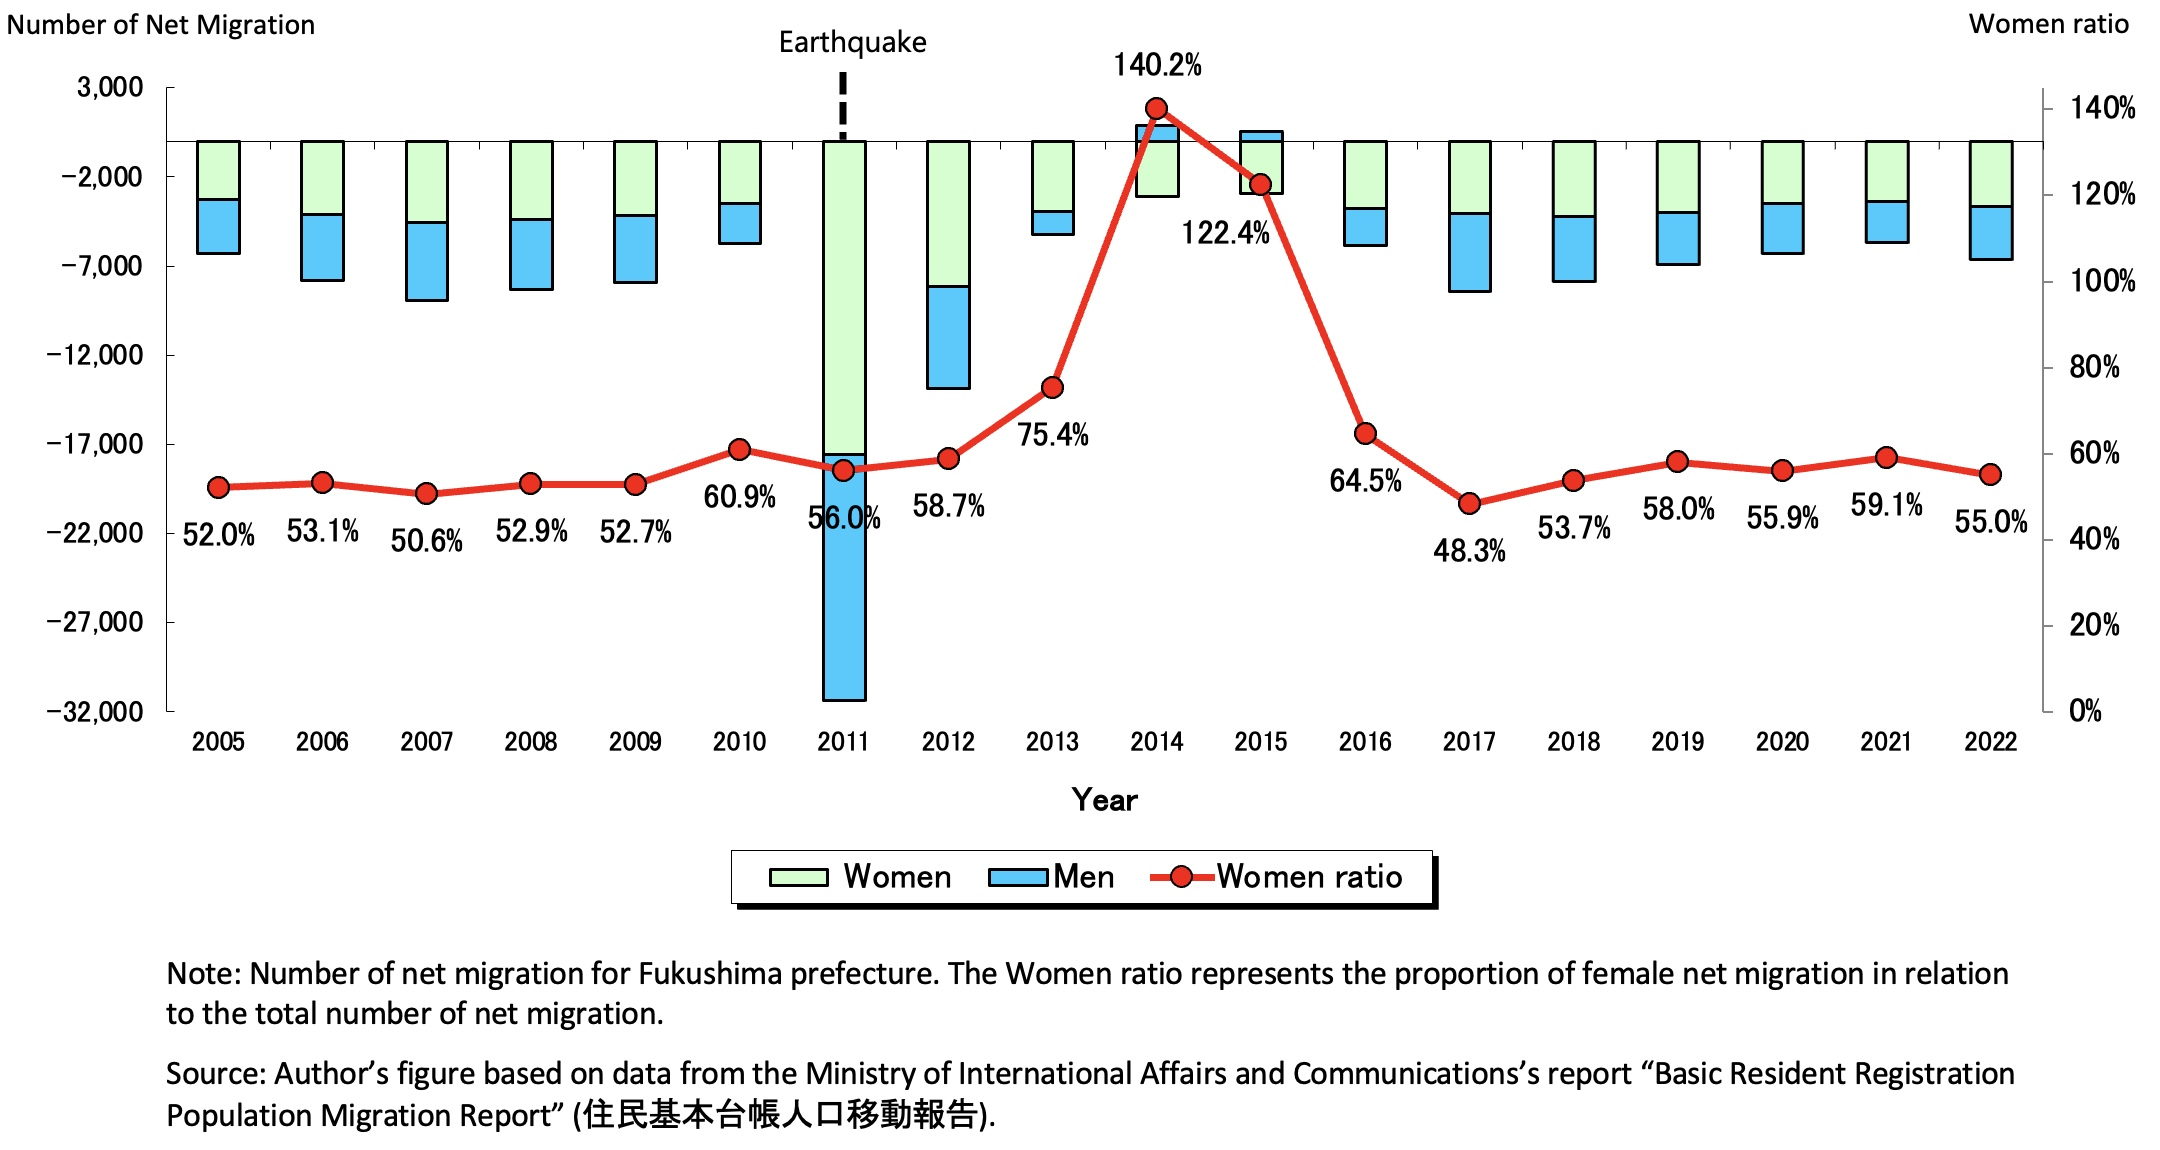
\includegraphics[width=0.70\textwidth]{Number of net migration.jpeg}  % 幅を本文の80%に設定
    \caption{The Number of Net Migration and The Proportion of Female Net Out-migration
to Total Net Out-migration in Fukushima Pref.}

\end{figure}

\vspace{-0.75cm}
\evacueeslinks


\end{frame}

%%%%%%%%%%%%%%%%%%%%%%%%%%%%%%%%
\section{Conclusion}
%%%%%%%%%%%%%%%%%%%%%%%%%%%%%%%%


\begin{frame}[label=summary]
\frametitle{Summary}
{\Large
\begin{itemize}
   \item The disaster's impact was highly heterogeneous across periods, genders, employment types, and industries.
   \item Initial phase: Women in the disaster area were more vulnerable to shocks (the risk adjustment hypothesis).
   \item Second phase: Women's average income increased faster than men's, due to a combination of selection bias and household shock coping strategies.
   \item Caution: Selection bias may lead to misleading policy implications if not properly addressed.
\end{itemize}
}
\end{frame}

%%%%%%%%%%%%%%%%%%%%%%%%%%%%%%%%


\begin{frame}[label=conclusion]

\frametitle{Conclusion}

    \begin{minipage}[c]{0.4\linewidth}
        \small

        \vspace{-1.6cm}
        

{\footnotesize
\begin{itemize}
    \item Phase 1: Women disproportionately affected due to prevalence in non-regular work(Risk Adjustment).
    \item Phase 2: Faster female recovery due to household coping strategies and selection bias(Evacuation changed the composition of women remaining in the area, introducing bias in the income).
    \item Phase 3: Returning to the steady state.
\end{itemize}

}

{\tiny
Magnitude of Impact:
}


{\tiny
\begin{equation}
\int_{T0}^{T2} [YF_F(t) - YF_C(t)] dt
\end{equation}
}

{\tiny
where $YF_F(t)$ represents the female worker's income in disaster affected area at time $t$, and $YF_C(t)$ represents the counterfactual which assumes the earthquake did not occur, assuming the parallel trend of control group.
}

        
        \vspace{-2.1cm}
        

    \end{minipage}\hspace{0.5cm}
    \begin{minipage}{0.2\linewidth}
        \medskip
        \begin{figure}[h]
            \centering
            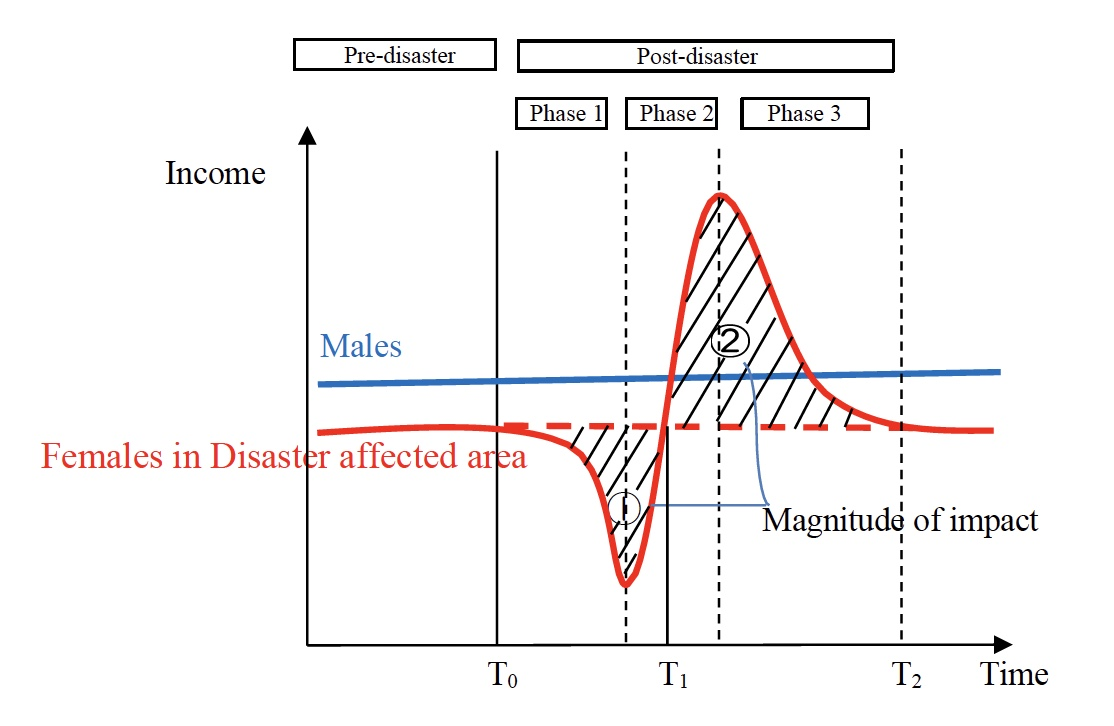
\includegraphics[height=.7\textheight]{Final_conceptual_model.jpeg}
        \end{figure}
    \end{minipage}

\conclusionlinks

\end{frame}


%%%%%%%%%%%%%%%%%%%%%%%%%%%%%%%%
%---------------------------------------
\begin{frame}
    \begin{center}
        {\Huge\calligra Thank You}
    \end{center}
\end{frame}
%---------------------------------------
%%%%%%%%%%%%%%%%%%%%%%%%%%%%%%%%


% アペンディックスセクションの開始
\appendix  % この行が重要です!

%%%%%%%%%%%%%%%%%%%%%%%%%%%%%%%%
\section{Appendix}
%%%%%%%%%%%%%%%%%%%%%%%%%%%%%%%%
\begin{frame}
    \centering
    \Huge \textbf{Appendix}
\end{frame}
%%%%%%%%%%%%%%%%%%%%%%%%%%%%%%%%%%%


\begin{frame}[label=unemploymentinsurance]
\frametitle{Short-term (upper graph) and long-term (lower graph) changes
in unemployment insurance recipients in Fukushima}

\vspace{0.25cm} 
\returnbutton{short_term_unemployment}{Return}


    \begin{minipage}[c]{0.4\linewidth}
        \small


        \vspace{-2.3cm}
        
        Reversal of Short-term and Long-term Trends:
        \begin{itemize}
            \item The ratio of women unemployment insurance recipients in Fukushima increased sharply after the disaster, surpassing the national average.

            \item However, in the longer term, the women's ratio in Fukushima fell below the national average, indicating a reversal of the initial trend.

        \end{itemize}
        
        \vspace{-2.1cm}
        

    \end{minipage}\hspace{0.5cm}
    \begin{minipage}{0.40\linewidth}
        \medskip
        \begin{figure}[h]
            \centering
            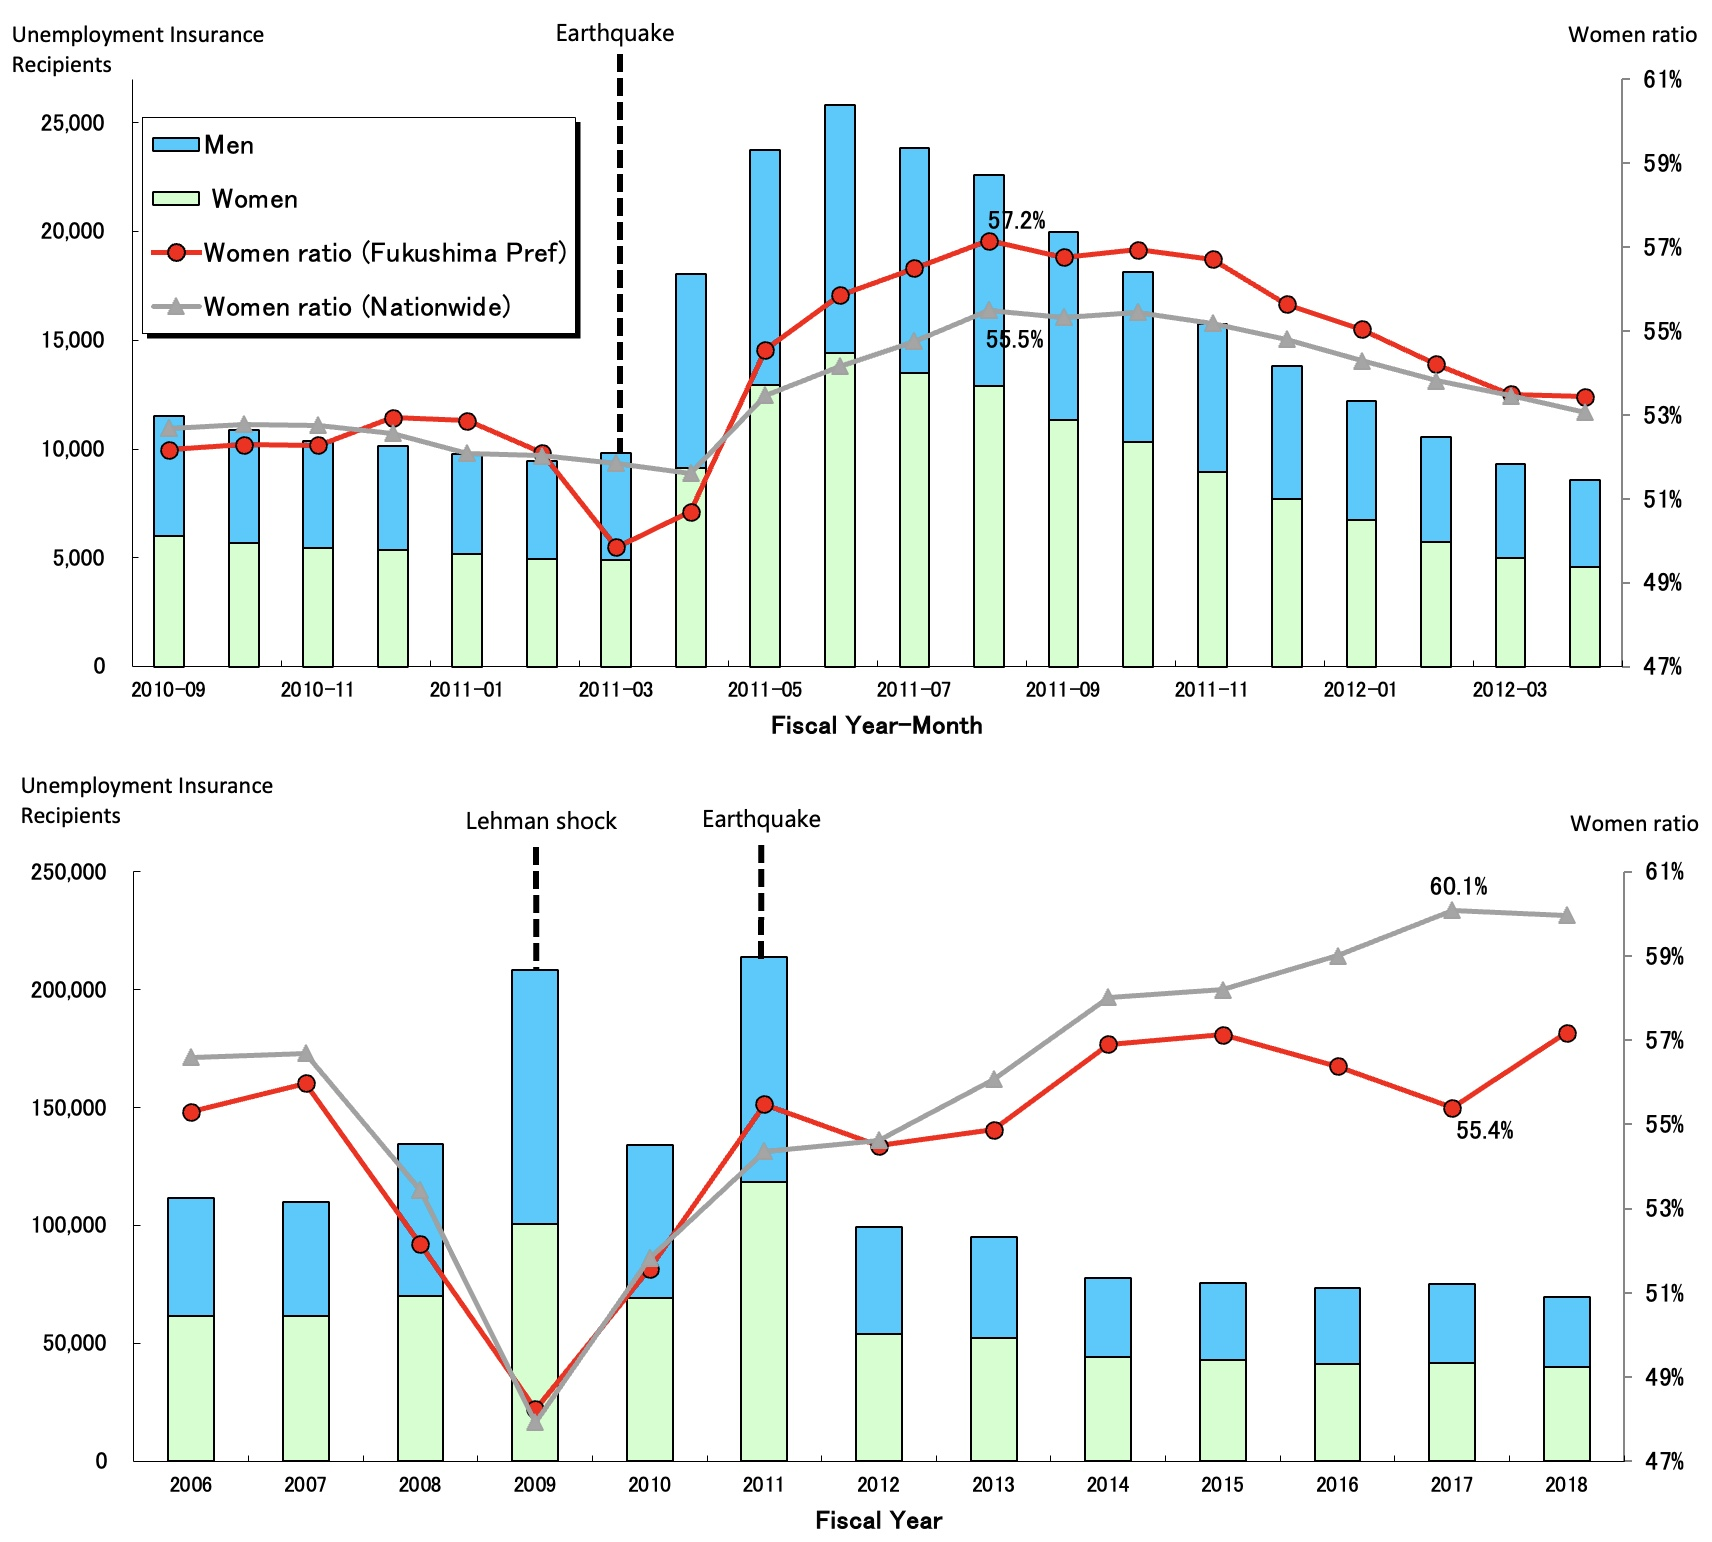
\includegraphics[height=.81\textheight]{Number of Actual Unemployment Insurance Recipients3.jpeg}
        \end{figure}
    \end{minipage}
\end{frame}
%%%%%%%%%%%%%%%%%%%%%%%%%%%%%%%%%%%

%---------------------------------------
% Slide: Literature Review - Risk Adjustment Hypothesis
%---------------------------------------

\begin{frame}[label=risk_adjustment_hypothesis]
\frametitle{Literature Review: Risk Adjustment Hypothesis}

\vspace{-1.0cm} 
\returnbutton{literature_review2}{Return}


    Nearly every empirical study of natural disasters finds short-term declines in either income or employment, especially for groups vulnerable to disasters, such as primary industry workers, non-regular workers, women, and the elderly.
    
    \vspace{0.3cm}
    
    \textbf{Key Studies:}
    \begin{itemize}
        \item \citet{Kim2014ARetention}: Analyzed the 2010 Haiti earthquake, revealing employment rates dropped from 52.6\% to 28.6\% five months post-disaster. Notably, only 34.2\% of women retained employment compared to 55.6\% of men.
        \item \citet{Groger2016InternalTyphoon}: Studied Typhoon Ketsana in Vietnam, finding affected households experienced a 10\% income decline due to crop losses. Internal labor migration to urban areas was a key coping mechanism.
    \end{itemize}
    
\end{frame}

%---------------------------------------
% Slide: Literature Review - Shock Coping Strategy
%---------------------------------------

\begin{frame}[label=shock_coping_strategy]
\frametitle{Literature Review: Shock Coping Strategy}

\vspace{0.2cm} 

\returnbutton{literature_review2}{Return}


    Development economics posits that households may increase labor supply as a strategy to cope with natural disasters, functioning as non-market insurance mechanisms essential for recovery and risk management.
    
    \vspace{0.3cm}
    
    \textbf{Key Studies:}
    \begin{itemize}
        \item \citet{Porcelli2019TheItaly}: Conducted a counterfactual analysis on 22 earthquakes in Italy (1986-2011), finding minimal economic contraction and sometimes positive net effects on output and employment due to reconstruction activities.
        \item \citet{Deryugina2018TheReturns}: Examined Hurricane Katrina's long-term impact on New Orleans residents, showing that income and employment rates eventually surpassed those of a control group.
        \item \citet{Canessa2021WomensShocks}: Demonstrated that severe flooding in Bangladesh increased women's employment probability by 13 percentage points, particularly among lower-income households and those involved in unpaid family farm work. This shift also enhanced household decision-making power for women.
    \end{itemize}
    
    \vspace{0.2cm}
    
    This study aims to fill gaps in the literature by differentiating between short-term and long-term effects of natural disasters on gender disparities, addressing contradictory findings regarding gender gap dynamics post-disaster.
    
\end{frame}

%---------------------------------------
% Slide: Literature Review - Theoretical Perspectives
%---------------------------------------

\begin{frame}[label=theoretical_perspective]
\frametitle{Literature Review: Theoretical Perspectives on Gender Disparities}

\vspace{0.2cm}

\returnbutton{literature_review2}{Return}

    \textbf{Theoretical Frameworks:}
    
    \vspace{0.1cm}
    
    \begin{columns}[T] % align columns
        \begin{column}{0.48\textwidth}
            \textbf{Risk Adjustment Hypothesis}
            
            \vspace{0.1cm}
            
            Suggests that during economic shocks or natural disasters, women are more susceptible to labor market exclusion and face higher risks of deteriorating work conditions or unemployment compared to men. This theory posits that women experience income reductions as they are disproportionately impacted by such adverse events.
        \end{column}
        \hfill
        \begin{column}{0.48\textwidth}
            \textbf{Shock Coping Strategy}
            
            \vspace{0.1cm}
            
            Proposes that households may respond to natural disasters by increasing labor supply as a coping mechanism. This strategy can lead to enhanced income opportunities for women, as they enter the workforce to mitigate income losses. Thus, this theory suggests a potential increase in women's income post-disaster.
        \end{column}
    \end{columns}
    
    \vspace{0.3cm}
    
    \textbf{Conflicting Findings:}
    
    While some studies support the Risk Adjustment Hypothesis, indicating a decline in women's employment and income, others align with the Shock Coping Strategy, showing an increase in women's labor force participation and income levels.

\end{frame}

%---------------------------------------
% Slide: Data
%---------------------------------------

\begin{frame}[label=data_full]
\frametitle{Data}

\vspace{-0.2cm}

\returnbutton{data}{Return}

    \vspace{-0.2cm}
  \begin{figure}
    \centering
    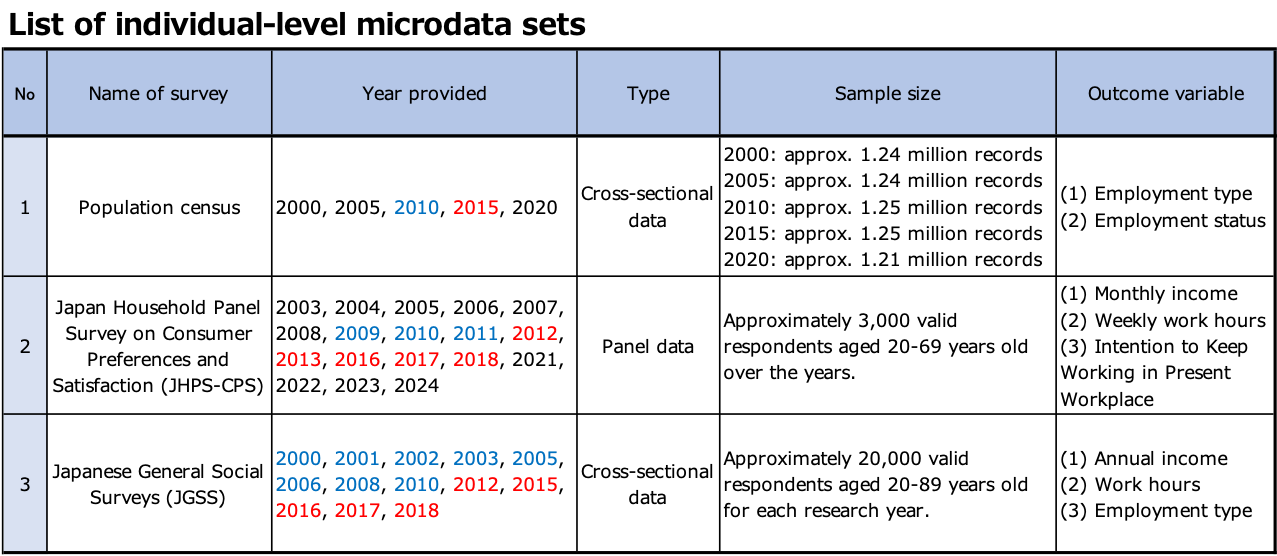
\includegraphics[width=0.93\textwidth]{list_of_individual_data.png}

  \end{figure}
\end{frame}

%---------------------------------------
% Slide: Ex. Real GRP growth rate
%---------------------------------------

\begin{frame}[label=real_GDP_growth_rate]

\frametitle{Real GRP growth rate over time: the affected prefectures (Treatment group) vs. Unaffected prefectures (Control group)}

\returnbutton{literature_review1}{Return}  % 特定のスライドにリンク

    \vspace{-0.06cm}
  \begin{figure}
    \centering
    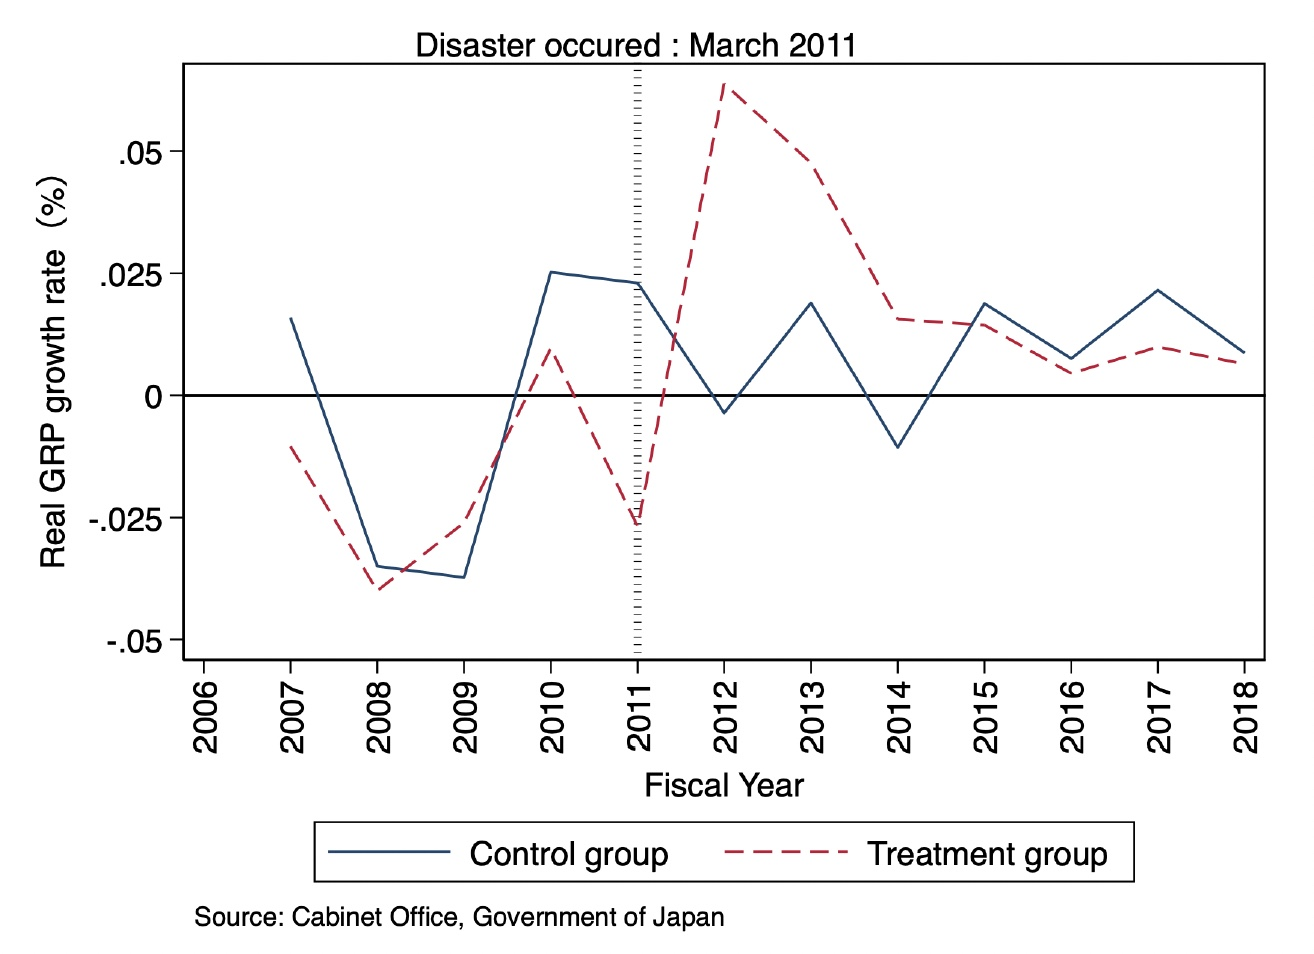
\includegraphics[width=0.62\textwidth]{Real GRP growth rate.jpeg}

  \end{figure}
\end{frame}

%%%%%%%%%%%%%%%%%%%%%%%%%%%%%%%%%%%%%%%%%

\begin{frame}[label=numbers_of_workers_full]

\vspace{0.4cm}

\returnbutton{numbers_of_workers}{Return}  % 特定のスライドにリンク

The significant
decrease in female non-regular employment may explain the substantial increase in average income for women post-disaster. (Population Census)

\begin{table}[htbp]
\centering
\caption{Difference in the Number of Workers (2010 vs 2015) in Fukushima}
%\scriptsize
%\tiny
\scalefont{0.31}  % 0.8は倍率。必要に応じて調整してください。
\begin{tabular}{l *{9}{S[table-format=-5.0]}}
\toprule
\multirow{3}{*}{Occupation} & {\multirow{3}{*}{\makecell[c]{\textbf{Total}\\\underline{(Reg +}\\\underline{Non-reg)}}}} & \multicolumn{4}{c}{\textbf{Regular}} & \multicolumn{4}{c}{\textbf{Non-regular}} \\
\cmidrule(lr){3-6} \cmidrule(lr){7-10}
& & {\multirow{2}{*}{\makecell[c]{\underline{Regular}\\\underline{(Total)}}}} & {Regular} & {Exec.} & {Self-} & {\multirow{2}{*}{\makecell[c]{\underline{Non-reg.}\\\underline{(Total)}}}} & {Disp.} & {Part-time,} & {Family} \\
& & & {empl.} & & {empl.} & & {workers} & {temp.} & {workers} \\
\midrule
\multicolumn{10}{c}{\textbf{Male}} \\
\midrule
Total & 1289 & -545 & 10591 & -1055 & -10081 & 1834 & 870 & 2719 & -1755 \\
Admin. \& managerial & -84 & -28 & -898 & 1296 & -426 & -52 & 0 & -52 & 0 \\
Prof. \& technical & 3521 & 3186 & 3400 & -119 & -95 & 335 & 112 & 263 & -40 \\
Clerical & 9364 & 7612 & 7251 & 276 & 85 & 1752 & 828 & 925 & -1 \\
Sales & -9636 & -8513 & -5186 & -1813 & -1514 & -1123 & -29 & -692 & -402 \\
Service & -1069 & -441 & 395 & -141 & -695 & -628 & 67 & -596 & -99 \\
Security & 1184 & 1094 & 1142 & -1 & -47 & 90 & 0 & 90 & 0 \\
Agri., forest. \& fish. & -6669 & -5959 & -383 & 32 & -5608 & -710 & -16 & -6 & -688 \\
Manufacturing & -14864 & -12017 & -10002 & -614 & -1401 & -2847 & -1668 & -768 & -411 \\
Trans. \& machine op. & 1042 & 596 & 747 & 19 & -170 & 446 & 122 & 308 & 16 \\
Constr. \& mining & 13740 & 11435 & 11403 & 85 & -53 & 2319 & 0 & 2211 & 108 \\
Carrying, clean., pack. & 7279 & 4519 & 4291 & -67 & 295 & 2760 & 1657 & 1179 & -76 \\
Not Classifiable & -2569 & -2049 & -1569 & 2 & -482 & -520 & -209 & -153 & -158 \\
\midrule
\multicolumn{10}{c}{\textbf{Female}} \\
\midrule
Total & -14626 & -1518 & 208 & 24 & -1750 & -13108 & -194 & -5413 & -7501 \\
Admin. \& managerial & 141 & 173 & -131 & 337 & -33 & -14 & 0 & -14 & 0 \\
Prof. \& technical & 2629 & 1957 & 2245 & 48 & -336 & 672 & -114 & 872 & -86 \\
Clerical & 4734 & 2516 & 2034 & 384 & 98 & 2218 & 921 & 1541 & -244 \\
Sales & -6188 & -2072 & -1053 & -489 & -530 & -4116 & -184 & -2580 & -1352 \\
Service & -2922 & 284 & 1496 & -140 & -1072 & -3206 & 27 & -2359 & -874 \\
Security & -33 & 87 & 72 & 8 & 7 & -120 & 0 & -120 & 0 \\
Agri., forest. \& fish. & -3950 & -127 & 10 & -17 & -120 & -3823 & -16 & -53 & -3754 \\
Manufacturing & -8632 & -4003 & -3494 & -73 & -436 & -4629 & -765 & -3236 & -628 \\
Trans. \& machine op. & 103 & 78 & 29 & -7 & 56 & 25 & -20 & 59 & -14 \\
Constr. \& mining & 328 & 96 & 124 & -27 & -1 & 222 & 0 & 208 & 14 \\
Carrying, clean., pack. & 646 & 12 & -329 & 33 & 308 & 634 & 26 & 537 & 71 \\
Not Classifiable & -1502 & -519 & -795 & -33 & 309 & -983 & -89 & -278 & -616 \\
\bottomrule
\end{tabular}

\addlinespace[0.35em]

\raggedright
\scriptsize

\end{table}

\end{frame}
%%%%%%%%%%%%%%%%%%%%%%%%%%%%%%%%



%%%%%%%%%%%%%%%%%%%%%%%%%%%%%%%%%%%%%


\begin{frame}[label=workers_number]

\vspace{0.4cm}

\returnbutton{employment_categories}{Return}  % 特定のスライドにリンク

\begin{table}[htbp]
\centering
\vspace{0.2em}
\caption{Number of workers by employment type and gender - Fukushima, Nationwide}

\resizebox{\textwidth}{!}{%
\begin{tabular}{lllllllllll}
\hline
\multirow{2}{*}{} & \multirow{2}{*}{\makecell[l]{Survey\\Year}} & \multirow{2}{*}{\makecell[l]{Total\\population}} & \multirow{2}{*}{\makecell[l]{Population of\\working age}} & \multirow{2}{*}{\makecell[l]{Total\\workers}} & \multirow{2}{*}{\makecell[l]{Regular\\employees}} & \multirow{2}{*}{\makecell[l]{Executives}} & \multirow{2}{*}{\makecell[l]{Self-\\employed}} & \multirow{2}{*}{\makecell[l]{Dispatched\\workers}} & \multirow{2}{*}{\makecell[l]{Part-time\\workers}} & \multirow{2}{*}{\makecell[l]{Family\\workers}} \\
 &  &  &  &  &  &  &  &  &  & \\
\hline
\addlinespace[0.5em]
\multicolumn{11}{l}{\textbf{Fukushima Pref}} \\
\addlinespace[0.5em]
Male & 2010 & 984,682 & 835,901 & \multicolumn{1}{l}{523,911} & \multicolumn{1}{l}{331,909} & \multicolumn{1}{l}{35,545} & \multicolumn{1}{l}{80,671} & \multicolumn{1}{l}{11,810} & \multicolumn{1}{l}{52,081} & \multicolumn{1}{l}{11,895} \\
 & 2015 & 945,660 (-4.0\%) & 813,542 (-2.7\%) & \multicolumn{1}{l}{525,200 (0.2\%)} & \multicolumn{1}{l}{342,500 (3.2\%)} & \multicolumn{1}{l}{34,490 (-3.0\%)} & \multicolumn{1}{l}{70,590 (-12.5\%)} & \multicolumn{1}{l}{12,680 (7.4\%)} & \multicolumn{1}{l}{54,800 (5.2\%)} & \multicolumn{1}{l}{10,140 (-14.8\%)} \\
 & 2020 & 903,864 (-8.2\%) & 777,758 (-6.9\%) & \multicolumn{1}{l}{477,770 (-8.8\%)} & \multicolumn{1}{l}{313,760 (-5.5\%)} & \multicolumn{1}{l}{35,330 (-0.6\%)} & \multicolumn{1}{l}{62,420 (-22.6\%)} & \multicolumn{1}{l}{10,040 (-15.0\%)} & \multicolumn{1}{l}{48,640 (-6.6\%)} & \multicolumn{1}{l}{7,580 (-36.3\%)} \\
\addlinespace[0.3em]
Female & 2010 & 1,044,382 & 905,008 & \multicolumn{1}{l}{400,036} & \multicolumn{1}{l}{162,482} & \multicolumn{1}{l}{12,336} & \multicolumn{1}{l}{21,410} & \multicolumn{1}{l}{12,224} & \multicolumn{1}{l}{148,763} & \multicolumn{1}{l}{42,821} \\
 & 2015 & 968,379 (-7.3\%) & 849,031 (-6.2\%) & \multicolumn{1}{l}{385,410 (-3.7\%)} & \multicolumn{1}{l}{162,690 (0.1\%)} & \multicolumn{1}{l}{12,360 (0.2\%)} & \multicolumn{1}{l}{19,660 (-8.2\%)} & \multicolumn{1}{l}{12,030 (-1.6\%)} & \multicolumn{1}{l}{143,350 (-3.6\%)} & \multicolumn{1}{l}{35,320 (-17.5\%)} \\
 & 2020 & 929,288 (-11.0\%) & 815,308 (-9.9\%) & \multicolumn{1}{l}{371,830 (-7.1\%)} & \multicolumn{1}{l}{166,900 (2.7\%)} & \multicolumn{1}{l}{12,320 (-0.1\%)} & \multicolumn{1}{l}{18,130 (-15.3\%)} & \multicolumn{1}{l}{10,430 (-14.7\%)} & \multicolumn{1}{l}{134,950 (-9.3\%)} & \multicolumn{1}{l}{29,100 (-32.0\%)} \\
\hline
\addlinespace[0.5em]
\multicolumn{11}{l}{\textbf{Nationwide}} \\
\addlinespace[0.5em]
Male & 2010 & 62,327,737 & 53,154,614 & \multicolumn{1}{l}{32,738,782} & \multicolumn{1}{l}{21,002,407} & \multicolumn{1}{l}{2,433,694} & \multicolumn{1}{l}{4,291,165} & \multicolumn{1}{l}{639,470} & \multicolumn{1}{l}{3,883,461} & \multicolumn{1}{l}{488,585} \\
 & 2015 & 61,841,738 (-0.8\%) & 52,879,791 (-0.5\%) & \multicolumn{1}{l}{31,720,790 (-3.1\%)} & \multicolumn{1}{l}{20,536,000 (-2.2\%)} & \multicolumn{1}{l}{2,213,220 (-9.1\%)} & \multicolumn{1}{l}{3,959,660 (-7.7\%)} & \multicolumn{1}{l}{652,830 (2.1\%)} & \multicolumn{1}{l}{3,942,620 (1.5\%)} & \multicolumn{1}{l}{416,460 (-14.8\%)} \\
 & 2020 & 61,349,581 (-1.6\%) & 52,098,467 (-2.0\%) & \multicolumn{1}{l}{30,871,667 (-5.7\%)} & \multicolumn{1}{l}{20,065,078 (-4.5\%)} & \multicolumn{1}{l}{2,364,280 (-2.9\%)} & \multicolumn{1}{l}{3,600,577 (-16.1\%)} & \multicolumn{1}{l}{638,324 (-0.2\%)} & \multicolumn{1}{l}{3,877,779 (-0.1\%)} & \multicolumn{1}{l}{325,629 (-33.4\%)} \\
\addlinespace[0.3em]
Female & 2010 & 65,729,615 & 57,122,871 & \multicolumn{1}{l}{24,627,898} & \multicolumn{1}{l}{9,433,752} & \multicolumn{1}{l}{746,640} & \multicolumn{1}{l}{1,286,990} & \multicolumn{1}{l}{891,120} & \multicolumn{1}{l}{10,436,445} & \multicolumn{1}{l}{1,832,951} \\
 & 2015 & 65,253,007 (-0.7\%) & 56,874,386 (-0.4\%) & \multicolumn{1}{l}{24,914,620 (1.2\%)} & \multicolumn{1}{l}{9,729,320 (3.1\%)} & \multicolumn{1}{l}{711,090 (-4.8\%)} & \multicolumn{1}{l}{1,247,870 (-3.0\%)} & \multicolumn{1}{l}{880,160 (-1.2\%)} & \multicolumn{1}{l}{10,795,720 (3.4\%)} & \multicolumn{1}{l}{1,550,460 (-15.4\%)} \\
 & 2020 & 64,796,518 (-1.4\%) & 56,160,102 (-1.7\%) & \multicolumn{1}{l}{25,675,371 (4.3\%)} & \multicolumn{1}{l}{10,731,753 (13.8\%)} & \multicolumn{1}{l}{769,919 (3.1\%)} & \multicolumn{1}{l}{1,264,299 (-1.8\%)} & \multicolumn{1}{l}{883,817 (-0.8\%)} & \multicolumn{1}{l}{10,745,470 (3.0\%)} & \multicolumn{1}{l}{1,280,113 (-30.2\%)} \\
\hline
\end{tabular}%
}
\addlinespace[0.12em]
\raggedright
\scriptsize
\textit{Note}: "Total workers" represent the number of workers in the population of working age (15 years and over) by gender for Fukushima Prefecture and Japan as a whole. Workers with "employment type not classifiable" are not included in the table and are excluded from the Total workers count. Percentages in parentheses represent the growth rate compared to the number of workers in 2010.\\
\textit{Source}: 2010, 2015 and 2020 Population Census.\\
\label{table:Number_of_workers}
\end{table}

\end{frame}

%%%%%%%%%%%%%%%%%%%%%%%%%%%%%%

\begin{frame}[fragile,label=appendix1]

\vspace{0.40cm} 
\returnbutton{proportion_of_employment_type}{Return}

\vspace{-0.30cm} 

\begin{figure}
\centering
\resizebox{0.96\textwidth}{!}{
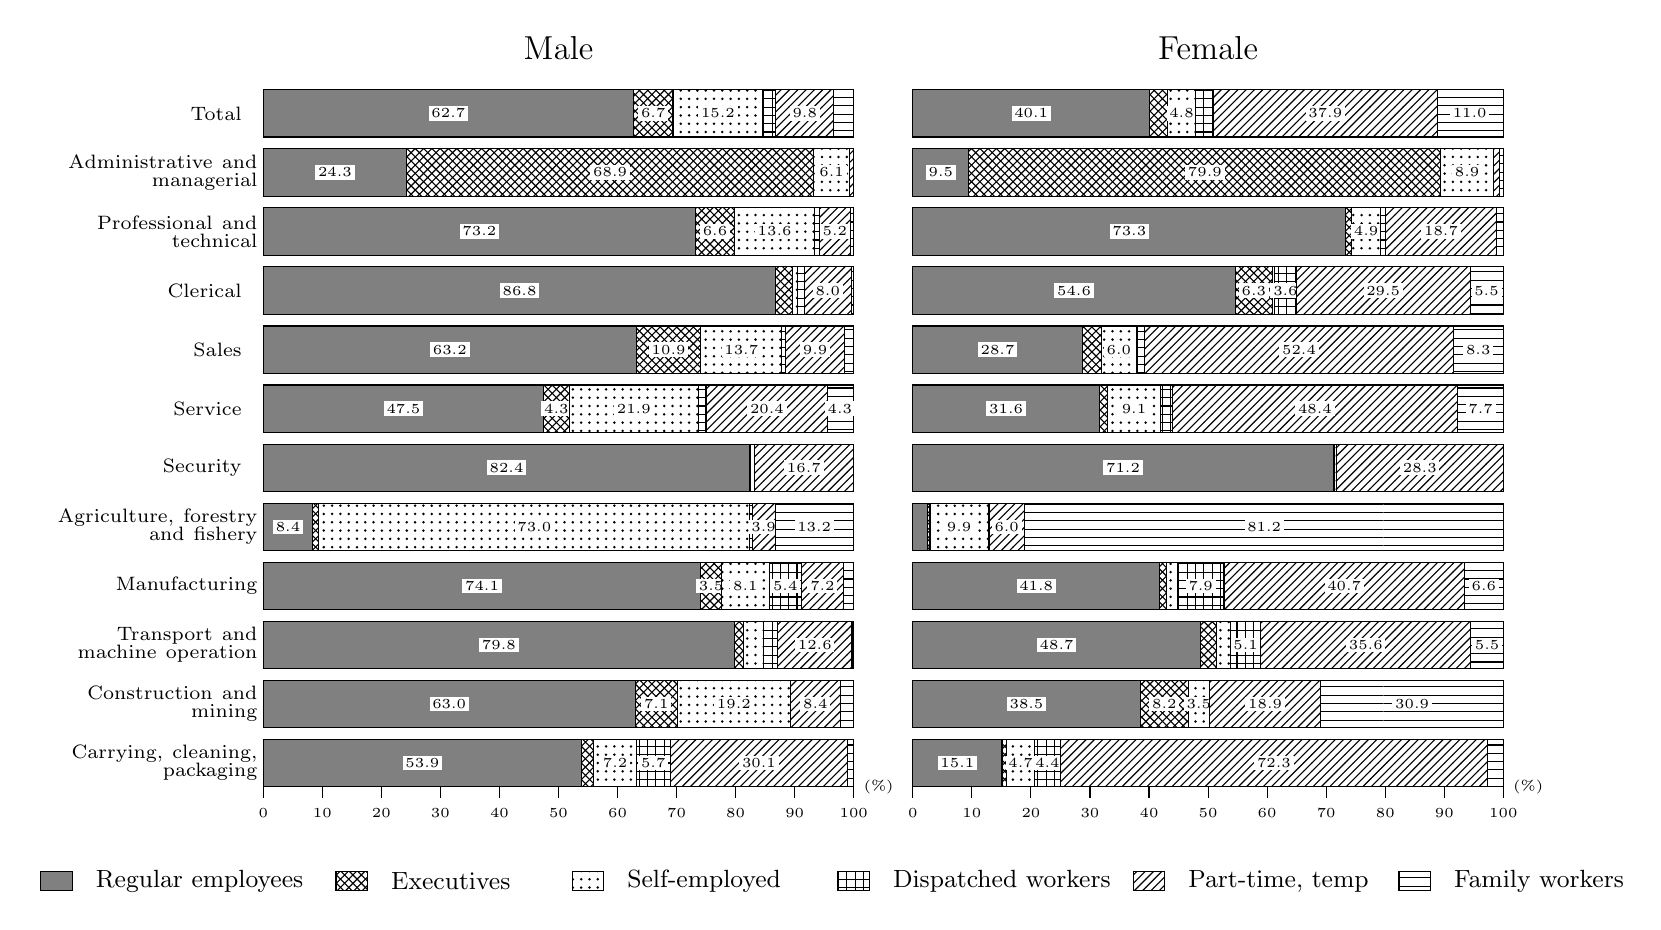
\begin{tikzpicture}[scale=0.75,xshift=-0.5cm]

% Define Colors
\definecolor{color1}{RGB}{128,128,128}
\definecolor{color2}{RGB}{200,200,200}
\definecolor{color3}{RGB}{220,220,220}
\definecolor{color4}{RGB}{180,180,180}
\definecolor{color5}{RGB}{100,100,100}
\definecolor{color6}{RGB}{60,60,60}

% Function to draw a stacked bar
\newcommand{\stackedbar}[8]{%
    \draw[fill=color1] (#1,#2) rectangle (#1+#3/10,#2+0.8);
    \pgfmathtruncatemacro{\resultA}{int(#3 >= 3.5 ? 1 : 0)}
    \ifnum\resultA>0
        \node[font=\tiny,fill=white,text=black,inner sep=1pt] at (#1+#3/20,#2+0.4) {#3};
    \fi
    \draw[fill=color2, pattern=crosshatch] (#1+#3/10,#2) rectangle (#1+#3/10+#4/10,#2+0.8);
    \pgfmathtruncatemacro{\resultB}{int(#4 >= 3.5 ? 1 : 0)}
    \ifnum\resultB>0
        \node[font=\tiny,fill=white,text=black,inner sep=1pt] at (#1+#3/10+#4/20,#2+0.4) {#4};
    \fi
    \draw[fill=color3, pattern=dots] (#1+#3/10+#4/10,#2) rectangle (#1+#3/10+#4/10+#5/10,#2+0.8);
    \pgfmathtruncatemacro{\resultC}{int(#5 >= 3.5 ? 1 : 0)}
    \ifnum\resultC>0
        \node[font=\tiny,fill=white,text=black,inner sep=1pt] at (#1+#3/10+#4/10+#5/20,#2+0.4) {#5};
    \fi
    \draw[fill=color4, pattern=grid] (#1+#3/10+#4/10+#5/10,#2) rectangle (#1+#3/10+#4/10+#5/10+#6/10,#2+0.8);
    \pgfmathtruncatemacro{\resultD}{int(#6 >= 3.5 ? 1 : 0)}
    \ifnum\resultD>0
        \node[font=\tiny,fill=white,text=black,inner sep=1pt] at (#1+#3/10+#4/10+#5/10+#6/20,#2+0.4) {#6};
    \fi
    \draw[fill=color5, pattern=north east lines] (#1+#3/10+#4/10+#5/10+#6/10,#2) rectangle (#1+#3/10+#4/10+#5/10+#6/10+#7/10,#2+0.8);
    \pgfmathtruncatemacro{\resultE}{int(#7 >= 3.5 ? 1 : 0)}
    \ifnum\resultE>0
        \node[font=\tiny,fill=white,text=black,inner sep=1pt] at (#1+#3/10+#4/10+#5/10+#6/10+#7/20,#2+0.4) {#7};
    \fi
    \draw[fill=color6, pattern=horizontal lines] (#1+#3/10+#4/10+#5/10+#6/10+#7/10,#2) rectangle (#1+10,#2+0.8);
    \pgfmathtruncatemacro{\resultF}{int(#8 >= 3.5 ? 1 : 0)}
    \ifnum\resultF>0
        \node[font=\tiny,fill=white,text=black,inner sep=1pt] at (#1+#3/10+#4/10+#5/10+#6/10+#7/10+#8/20,#2+0.4) {#8};
    \fi
}

% Male bars
\begin{scope}[xshift=-5.5cm]
    \stackedbar{0}{11}{62.7}{6.7}{15.2}{2.2}{9.8}{2.3}
    \node[anchor=east, text width=2.6cm, align=right] at (-0.2,11.4) {\scriptsize Total};
    
    \stackedbar{0}{10}{24.3}{68.9}{6.1}{0}{0.7}{0}
    \node[anchor=east, text width=2.6cm, align=right] at (-0.2,10.4) {\scriptsize\parbox[t]{2.8cm}{\setstretch{0.8}\raggedleft Administrative and managerial}};
    
    \stackedbar{0}{9}{73.2}{6.6}{13.6}{0.8}{5.2}{0.6}
    \node[anchor=east, text width=2.6cm, align=right] at (-0.2,9.4) {\scriptsize\parbox[t]{2.8cm}{\setstretch{0.8}\raggedleft Professional and technical}};
    
    \stackedbar{0}{8}{86.8}{2.9}{0.7}{1.2}{8.0}{0.3}
    \node[anchor=east, text width=2.6cm, align=right] at (-0.2,8.4) {\scriptsize Clerical};
    
    \stackedbar{0}{7}{63.2}{10.9}{13.7}{0.7}{9.9}{1.6}
    \node[anchor=east, text width=2.6cm, align=right] at (-0.2,7.4) {\scriptsize Sales};
    
    \stackedbar{0}{6}{47.5}{4.3}{21.9}{1.4}{20.4}{4.3}
    \node[anchor=east, text width=2.6cm, align=right] at (-0.2,6.4) {\scriptsize Service};
    
    \stackedbar{0}{5}{82.4}{0.1}{0.7}{0}{16.7}{0}
    \node[anchor=east, text width=2.6cm, align=right] at (-0.2,5.4) {\scriptsize Security};
    
    \stackedbar{0}{4}{8.4}{1.0}{73.0}{0.4}{3.9}{13.2}
    \node[anchor=east, text width=2.6cm, align=right] at (-0.2,4.4) {\scriptsize\parbox[t]{2.8cm}{\setstretch{0.8}\raggedleft Agriculture, forestry and fishery}};
    
    \stackedbar{0}{3}{74.1}{3.5}{8.1}{5.4}{7.2}{1.5}
    \node[anchor=east, text width=2.6cm, align=right] at (-0.2,3.4) {\scriptsize\parbox[t]{2.8cm}{\setstretch{0.8}\raggedleft Manufacturing}};
    
    \stackedbar{0}{2}{79.8}{1.5}{3.4}{2.4}{12.6}{0.2}
    \node[anchor=east, text width=2.6cm, align=right] at (-0.2,2.4) {\scriptsize\parbox[t]{2.8cm}{\setstretch{0.8}\raggedleft Transport and machine operation}};
    
    \stackedbar{0}{1}{63.0}{7.1}{19.2}{0}{8.4}{2.2}
    \node[anchor=east, text width=2.6cm, align=right] at (-0.2,1.4) {\scriptsize\parbox[t]{2.8cm}{\setstretch{0.8}\raggedleft Construction and mining}};
    
    \stackedbar{0}{0}{53.9}{2.1}{7.2}{5.7}{30.1}{1.0}
    \node[anchor=east, text width=2.6cm, align=right] at (-0.2,0.4) {\scriptsize\parbox[t]{2.8cm}{\setstretch{0.8}\raggedleft Carrying, cleaning, packaging}};
    
    % X-axis for Male
    \draw (0,0) -- (10,0);
    \foreach \x in {0,1,...,10} {
        \draw (\x,0) -- (\x,-0.2) 
            node[anchor=north] {\tiny \ifnum\x=0 0\else\x0\fi};
    }
    \node[anchor=west] at (10,0) {\tiny (\%)};
    
    % Label for Male
    \node[anchor=center] at (5,12.5) {\large Male};
\end{scope}

% Female bars
\begin{scope}[xshift=5.5cm]
    \stackedbar{0}{11}{40.1}{3.0}{4.8}{3.0}{37.9}{11.0}
    \stackedbar{0}{10}{9.5}{79.9}{8.9}{0}{1.1}{0.6}
    \stackedbar{0}{9}{73.3}{1.0}{4.9}{0.9}{18.7}{1.2}
    \stackedbar{0}{8}{54.6}{6.3}{0.4}{3.6}{29.5}{5.5}
    \stackedbar{0}{7}{28.7}{3.2}{6.0}{1.3}{52.4}{8.3}
    \stackedbar{0}{6}{31.6}{1.3}{9.1}{1.9}{48.4}{7.7}
    \stackedbar{0}{5}{71.2}{0.2}{0.3}{0}{28.3}{0}
    \stackedbar{0}{4}{2.5}{0.4}{9.9}{0.1}{6.0}{81.2}
    \stackedbar{0}{3}{41.8}{1.1}{1.9}{7.9}{40.7}{6.6}
    \stackedbar{0}{2}{48.7}{2.7}{2.4}{5.1}{35.6}{5.5}
    \stackedbar{0}{1}{38.5}{8.2}{3.5}{0}{18.9}{30.9}
    \stackedbar{0}{0}{15.1}{0.8}{4.7}{4.4}{72.3}{2.8}
    
    % X-axis for Female
    \draw (0,0) -- (10,0);
    \foreach \x in {0,1,...,10} {
        \draw (\x,0) -- (\x,-0.2) 
            node[anchor=north] {\tiny \ifnum\x=0 0\else\x0\fi};
    }
    \node[anchor=west] at (10,0) {\tiny (\%)};
    
    % Label for Female
    \node[anchor=center] at (5,12.5) {\large Female};
\end{scope}

\vspace{-0.50cm} 

% Legend (1 row, 6 columns)
\node[anchor=center, fill=color1, minimum width=0.4cm, minimum height=0.2cm, draw] at (-9,-1.6) {};
\node[anchor=west] at (-8.5,-1.6) {\small Regular employees};
\node[anchor=center, fill=color2, pattern=crosshatch, minimum width=0.4cm, minimum height=0.2cm, draw] at (-4,-1.6) {};
\node[anchor=west] at (-3.5,-1.6) {\small Executives};
\node[anchor=center, fill=color3, pattern=dots, minimum width=0.4cm, minimum height=0.2cm, draw] at (0,-1.6) {};
\node[anchor=west] at (0.5,-1.6) {\small Self-employed};
\node[anchor=center, fill=color4, pattern=grid, minimum width=0.4cm, minimum height=0.2cm, draw] at (4.5,-1.6) {};
\node[anchor=west] at (5,-1.6) {\small Dispatched workers};
\node[anchor=center, fill=color5, pattern=north east lines, minimum width=0.4cm, minimum height=0.2cm, draw] at (9.5,-1.6) {};
\node[anchor=west] at (10,-1.6) {\small Part-time, temp};
\node[anchor=center, fill=color6, pattern=horizontal lines, minimum width=0.4cm, minimum height=0.2cm, draw] at (14,-1.6) {};
\node[anchor=west] at (14.5,-1.6) {\small Family workers};


\end{tikzpicture}
}
%\caption{Proportion of Employed Persons Aged 15 and Over by Occupation, Employment types, and Gender - Fukushima Prefecture (2010)}
\end{figure}

\end{frame}

%%%%%%%%%%%%%%%%%%%%%%%%%%%%%%%%%%%%%%%%%%

\begin{frame}[label=appendix2]

\frametitle{Proportion of Employed Persons by Industry - Fukushima (2010)}

\vspace{0.20cm} 

\returnbutton{proportion_of_employment_type}{Return}  % 特定のスライドにリンク

\begin{figure}[htbp]
    \centering 
    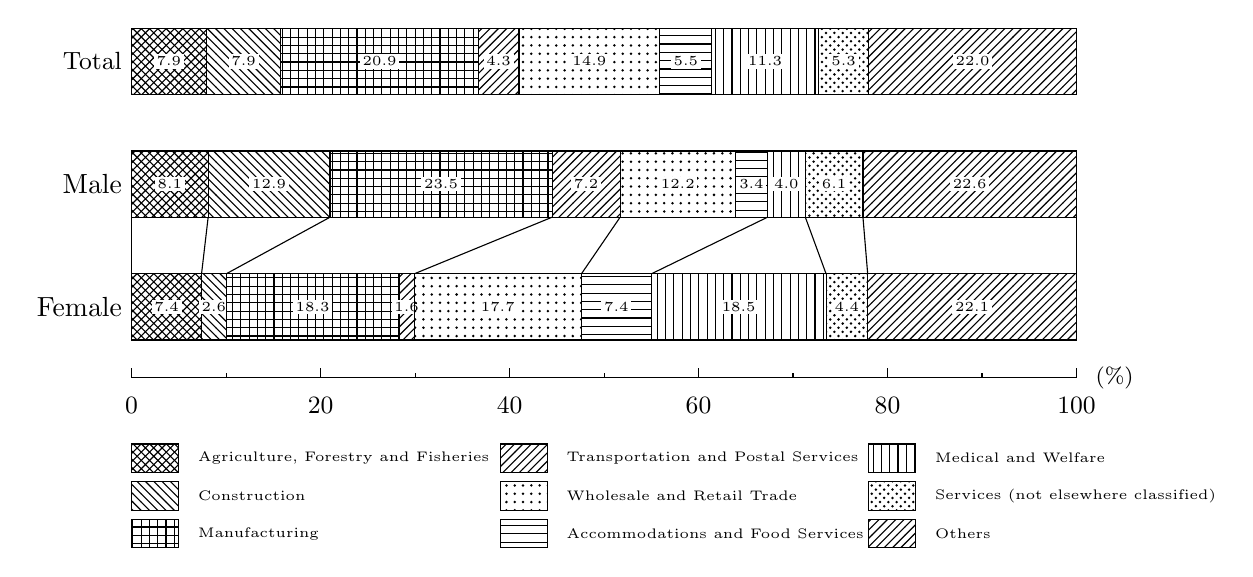
\begin{tikzpicture}[scale=1.20]
    % 色の定義
    \definecolor{color1}{RGB}{200,200,200} 
    \definecolor{color2}{RGB}{150,150,150} 
    \definecolor{color3}{RGB}{100,100,100}
    \definecolor{color4}{RGB}{250,200,200}
    \definecolor{color5}{RGB}{200,150,150}
    \definecolor{color6}{RGB}{150,100,100}
    \definecolor{color7}{RGB}{100,50,50}
    \definecolor{color8}{RGB}{50,0,0}
    \definecolor{color9}{RGB}{0,0,0}
    
    % 棒グラフの描画
    % Total bar
    \draw[fill=color1, pattern=crosshatch] (2,9) rectangle (2.79,9.7) node[pos=0.5, fill=white, inner sep=1pt] {\tiny 7.9};
    \draw[fill=color2, pattern=north west lines] (2.79,9) rectangle (3.58,9.7) node[pos=0.5, fill=white, inner sep=1pt] {\tiny 7.9};
    \draw[fill=color3, pattern=grid] (3.58,9) rectangle (5.67,9.7) node[pos=0.5, fill=white, inner sep=1pt] {\tiny 20.9};
    \draw[fill=color4, pattern=north east lines] (5.67,9) rectangle (6.10,9.7) node[pos=0.5, fill=white, inner sep=1pt] {\tiny 4.3}; 
    \draw[fill=color5, pattern=dots] (6.10,9) rectangle (7.59,9.7) node[pos=0.5, fill=white, inner sep=1pt] {\tiny 14.9}; 
    \draw[fill=color6, pattern=horizontal lines] (7.59,9) rectangle (8.14,9.7) node[pos=0.5, fill=white, inner sep=1pt] {\tiny 5.5};
    \draw[fill=color7, pattern=vertical lines] (8.14,9) rectangle (9.27,9.7) node[pos=0.5, fill=white, inner sep=1pt] {\tiny 11.3};
    \draw[fill=color8, pattern=crosshatch dots] (9.27,9) rectangle (9.80,9.7) node[pos=0.5, fill=white, inner sep=1pt] {\tiny 5.3};
    \draw[fill=color9, pattern=north east lines] (9.80,9) rectangle (12,9.7) node[pos=0.5, fill=white, inner sep=1pt] {\tiny 22.0}; 
    
    % Male bar
    \draw[fill=color1, pattern=crosshatch] (2,7.7) rectangle (2.81,8.4) node[pos=0.5, fill=white, inner sep=1pt] {\tiny 8.1};
    \draw[fill=color2, pattern=north west lines] (2.81,7.7) rectangle (4.10,8.4) node[pos=0.5, fill=white, inner sep=1pt] {\tiny 12.9};
    \draw[fill=color3, pattern=grid] (4.10,7.7) rectangle (6.45,8.4) node[pos=0.5, fill=white, inner sep=1pt] {\tiny 23.5};
    \draw[fill=color4, pattern=north east lines] (6.45,7.7) rectangle (7.17,8.4) node[pos=0.5, fill=white, inner sep=1pt] {\tiny 7.2}; 
    \draw[fill=color5, pattern=dots] (7.17,7.7) rectangle (8.39,8.4) node[pos=0.5, fill=white, inner sep=1pt] {\tiny 12.2}; 
    \draw[fill=color6, pattern=horizontal lines] (8.39,7.7) rectangle (8.73,8.4) node[pos=0.5, fill=white, inner sep=1pt] {\tiny 3.4};
    \draw[fill=color7, pattern=vertical lines] (8.73,7.7) rectangle (9.13,8.4) node[pos=0.5, fill=white, inner sep=1pt] {\tiny 4.0};
    \draw[fill=color8, pattern=crosshatch dots] (9.13,7.7) rectangle (9.74,8.4) node[pos=0.5, fill=white, inner sep=1pt] {\tiny 6.1};
    \draw[fill=color9, pattern=north east lines] (9.74,7.7) rectangle (12,8.4) node[pos=0.5, fill=white, inner sep=1pt] {\tiny 22.6};
    
    % Female bar
    \draw[fill=color1, pattern=crosshatch] (2,6.4) rectangle (2.74,7.1) node[pos=0.5, fill=white, inner sep=1pt] {\tiny 7.4};
    \draw[fill=color2, pattern=north west lines] (2.74,6.4) rectangle (3.00,7.1) node[pos=0.5, fill=white, inner sep=1pt] {\tiny 2.6};
    \draw[fill=color3, pattern=grid] (3.00,6.4) rectangle (4.83,7.1) node[pos=0.5, fill=white, inner sep=1pt] {\tiny 18.3};
    \draw[fill=color4, pattern=north east lines] (4.83,6.4) rectangle (4.99,7.1) node[pos=0.5, fill=white, inner sep=1pt] {\tiny 1.6}; 
    \draw[fill=color5, pattern=dots] (4.99,6.4) rectangle (6.76,7.1) node[pos=0.5, fill=white, inner sep=1pt] {\tiny 17.7}; 
    \draw[fill=color6, pattern=horizontal lines] (6.76,6.4) rectangle (7.50,7.1) node[pos=0.5, fill=white, inner sep=1pt] {\tiny 7.4};
    \draw[fill=color7, pattern=vertical lines] (7.50,6.4) rectangle (9.35,7.1) node[pos=0.5, fill=white, inner sep=1pt] {\tiny 18.5};
    \draw[fill=color8, pattern=crosshatch dots] (9.35,6.4) rectangle (9.79,7.1) node[pos=0.5, fill=white, inner sep=1pt] {\tiny 4.4};
    \draw[fill=color9, pattern=north east lines] (9.79,6.4) rectangle (12,7.1) node[pos=0.5, fill=white, inner sep=1pt] {\tiny 22.1}; 
    
    % ガイドラインの描画(Maleのバーの下端からFemaleのバーの上端へ)
    \draw[thin] (2,7.7) -- (2,7.1);
    \draw[thin] (2.81,7.7) -- (2.74,7.1);
    \draw[thin] (4.10,7.7) -- (3.00,7.1);
    \draw[thin] (6.45,7.7) -- (4.99,7.1);
    \draw[thin] (7.17,7.7) -- (6.76,7.1);
    \draw[thin] (8.73,7.7) -- (7.50,7.1);
    \draw[thin] (9.13,7.7) -- (9.35,7.1);
    \draw[thin] (9.74,7.7) -- (9.79,7.1);
    \draw[thin] (12,7.7) -- (12,7.1);
    
    % ラベルの描画(フォントサイズを調整)
    \node[anchor=east, font=\small] at (2,9.35) {Total};
    \node[anchor=east, font=\normalsize] at (2,8.05) {Male};
    \node[anchor=east, font=\normalsize] at (2,6.75) {Female};
    
    % X軸の描画
    \draw (2,6) -- (12,6);
    \foreach \x in {0,20,40,60,80,100} {
        \draw (2+\x/10,6) -- (2+\x/10,6.1) 
            node[anchor=north] at (2+\x/10,5.9) {\small \x};
    }
    \foreach \x in {10,30,50,70,90} {
        \draw (2+\x/10,6) -- (2+\x/10,6.05);
    }
    \node[anchor=west, font=\footnotesize] at (12.1,6) {(\%)};
    
    % 凡例の描画(手動で作成)
    \begin{scope}[shift={(0,5.0)}] % 凡例の位置を調整
        % 列間の間隔を1.3倍に拡大(x=2, 5.9, 9.8)
        
        % 列1
        \draw[fill=color1, pattern=crosshatch, minimum width=0.5cm, minimum height=0.3cm, draw] (2,0) rectangle ++(0.5,0.3);
        \node[anchor=west, font=\tiny] at (2.6,0.15) {Agriculture, Forestry and Fisheries};
        
        \draw[fill=color2, pattern=north west lines, minimum width=0.5cm, minimum height=0.3cm, draw] (2,-0.4) rectangle ++(0.5,0.3);
        \node[anchor=west, font=\tiny] at (2.6,-0.25) {Construction};
        
        \draw[fill=color3, pattern=grid, minimum width=0.5cm, minimum height=0.3cm, draw] (2,-0.8) rectangle ++(0.5,0.3);
        \node[anchor=west, font=\tiny] at (2.6,-0.65) {Manufacturing};
        
        % 列2 (x=5.9)
        \draw[fill=color4, pattern=north east lines, minimum width=0.5cm, minimum height=0.3cm, draw] (5.9,0) rectangle ++(0.5,0.3);
        \node[anchor=west, font=\tiny] at (6.5,0.15) {Transportation and Postal Services};
        
        \draw[fill=color5, pattern=dots, minimum width=0.5cm, minimum height=0.3cm, draw] (5.9,-0.4) rectangle ++(0.5,0.3);
        \node[anchor=west, font=\tiny] at (6.5,-0.25) {Wholesale and Retail Trade};
        
        \draw[fill=color6, pattern=horizontal lines, minimum width=0.5cm, minimum height=0.3cm, draw] (5.9,-0.8) rectangle ++(0.5,0.3);
        \node[anchor=west, font=\tiny] at (6.5,-0.65) {Accommodations and Food Services};
        
        % 列3 (x=9.8)
        \draw[fill=color7, pattern=vertical lines, minimum width=0.5cm, minimum height=0.3cm, draw] (9.8,0) rectangle ++(0.5,0.3);
        \node[anchor=west, font=\tiny] at (10.4,0.15) {Medical and Welfare};
        
        \draw[fill=color8, pattern=crosshatch dots, minimum width=0.5cm, minimum height=0.3cm, draw] (9.8,-0.4) rectangle ++(0.5,0.3);
        \node[anchor=west, font=\tiny] at (10.4,-0.25) {Services (not elsewhere classified)};
        
        \draw[fill=color9, pattern=north east lines, minimum width=0.5cm, minimum height=0.3cm, draw] (9.8,-0.8) rectangle ++(0.5,0.3);
        \node[anchor=west, font=\tiny] at (10.4,-0.65) {Others};
    \end{scope}
    
    \end{tikzpicture} 
    % \caption{Proportion of Employed Persons Aged 15 and Over by Industry and Sex - Fukushima (2010)} % \captionを削除
\end{figure}

\end{frame}

%%%%%%%%%%%%%%%%%

% Gender gap by Industry
%%%%%%%%%%%%%%%%%%%%%%%%%%


\begin{frame}[label=appendix3]
\frametitle{Proportion of Employed Persons - Fukushima Pref (2010)}

\vspace{0.20cm} 

\returnbutton{numbers_of_workers}{Return}  % 特定のスライドにリンク


\begin{figure}[!t]
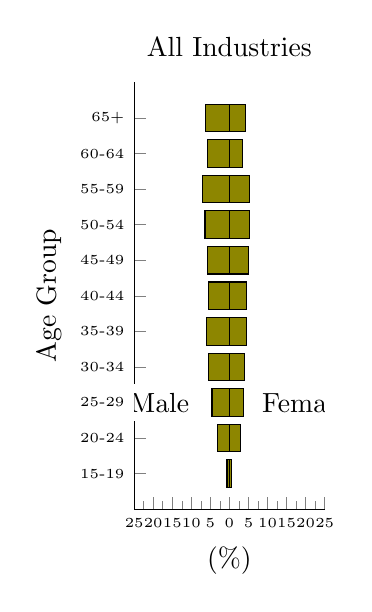
\begin{tikzpicture}
\begin{axis}[
    width=0.33\textwidth,
    height=7cm,
    xbar stacked,
    xmin=-25,
    xmax=25,
    xtick={-25, -20, -15, -10, -5, 0, 5, 10, 15, 20, 25},
    xticklabels={25, 20, 15, 10, 5, 0, 5, 10, 15, 20, 25},
    xlabel={(\%)},
    ylabel={Age Group},
    ytick={1,2,3,4,5,6,7,8,9,10,11},
    yticklabels={15-19, 20-24, 25-29, 30-34, 35-39, 40-44, 45-49, 50-54, 55-59, 60-64, 65+},
    title={All Industries},
    axis y line*=left,
    axis x line*=bottom,
    bar width=3.5mm,
    xticklabel style={font=\tiny},
    yticklabel style={font=\tiny},
    xlabel style={font=\normalsize},
    minor x tick num=1,
    grid style={line width=.1pt, draw=gray!20},
    major grid style={line width=.2pt,draw=gray!50},
]
\addplot[xbar, fill=olive] coordinates {(-6.2968,11) (-5.7348,10) (-7.0630,9) (-6.4160,8) (-5.8457,7) (-5.4109,6) (-6.0469,5) (-5.5079,4) (-4.5710,3) (-3.1366,2) (-0.6502,1)};
\addplot[xbar, fill=olive] coordinates {(4.1861,11) (3.5393,10) (5.1758,9) (5.2826,8) (4.9579,7) (4.4568,6) (4.5115,5) (4.0165,4) (3.6677,3) (2.9304,2) (0.5957,1)};
\node[anchor=east, fill=white] at (axis cs:-8,3) {Male};
\node[anchor=west, fill=white] at (axis cs:6,3) {Female};
\end{axis}
\end{tikzpicture}
\hfill
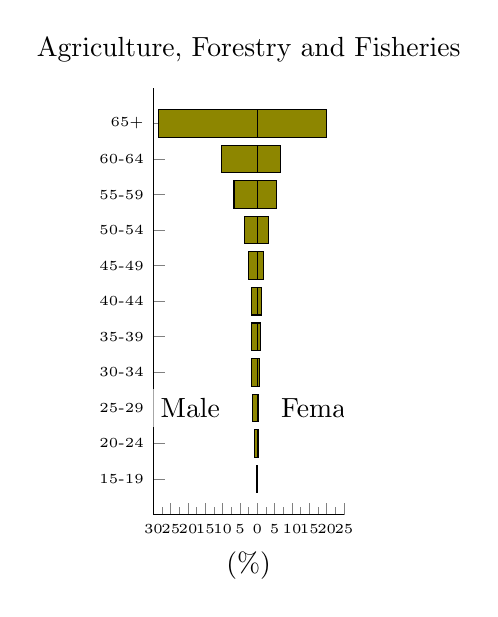
\begin{tikzpicture}
\begin{axis}[
    width=0.33\textwidth,
    height=7cm,
    xbar stacked,
    xmin=-30,
    xmax=25,
    xtick={-30, -25, -20, -15, -10, -5, 0, 5, 10, 15, 20, 25},
    xticklabels={30, 25, 20, 15, 10, 5, 0, 5, 10, 15, 20, 25},
    xlabel={(\%)},
    ytick={1,2,3,4,5,6,7,8,9,10,11},
    yticklabels={15-19, 20-24, 25-29, 30-34, 35-39, 40-44, 45-49, 50-54, 55-59, 60-64, 65+},
    yticklabel pos=right,
    title={Agriculture, Forestry and Fisheries},
    axis y line*=left,
    axis x line*=bottom,
    bar width=3.5mm,
    xticklabel style={font=\tiny},
    yticklabel style={font=\tiny},
    xlabel style={font=\normalsize},
    minor x tick num=1,
    grid style={line width=.1pt, draw=gray!20},
    major grid style={line width=.2pt,draw=gray!50},
]
\addplot[xbar, fill=olive] coordinates {(-28.5896,11) (-10.3951,10) (-6.7607,9) (-3.8248,8) (-2.5634,7) (-1.6352,6) (-1.6058,5) (-1.6520,4) (-1.2908,3) (-0.8218,2) (-0.1694,1)};
\addplot[xbar, fill=olive] coordinates {(20.0734,11) (6.5899,10) (5.5664,9) (3.2718,8) (1.7640,7) (1.1144,6) (0.8792,5) (0.6888,4) (0.4494,3) (0.2394,2) (0.0546,1)};
\node[anchor=east, fill=white] at (axis cs:-8,3) {Male};
\node[anchor=west, fill=white] at (axis cs:4,3) {Female};
\end{axis}
\end{tikzpicture}
\hfill
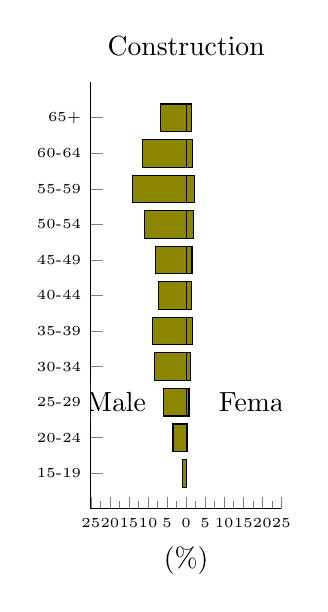
\begin{tikzpicture}
\begin{axis}[
    width=0.33\textwidth,
    height=7cm,
    xbar stacked,
    xmin=-25,
    xmax=25,
    xtick={-25, -20, -15, -10, -5, 0, 5, 10, 15, 20, 25},
    xticklabels={25, 20, 15, 10, 5, 0, 5, 10, 15, 20, 25},
    xlabel={(\%)},
    ytick={1,2,3,4,5,6,7,8,9,10,11},
    yticklabels={15-19, 20-24, 25-29, 30-34, 35-39, 40-44, 45-49, 50-54, 55-59, 60-64, 65+},
    yticklabel pos=right,
    title={Construction},
    axis y line*=left,
    axis x line*=bottom,
    bar width=3.5mm,
    xticklabel style={font=\tiny},
    yticklabel style={font=\tiny},
    xlabel style={font=\normalsize},
    minor x tick num=1,
    grid style={line width=.1pt, draw=gray!20},
    major grid style={line width=.2pt,draw=gray!50},
]
\addplot[xbar, fill=olive] coordinates {(-6.6875,11) (-11.4525,10) (-14.1118,9) (-10.9621,8) (-8.1361,7) (-7.1541,6) (-8.9182,5) (-8.3385,4) (-6.0411,3) (-3.4449,2) (-0.8749,1)};
\addplot[xbar, fill=olive] coordinates {(1.2939,11) (1.7058,10) (2.1069,9) (1.8165,8) (1.5332,7) (1.4439,6) (1.6165,5) (1.2035,4) (0.7380,3) (0.3726,2) (0.0476,1)};
\node[anchor=east, fill=white] at (axis cs:-8,3) {Male};
\node[anchor=west, fill=white] at (axis cs:6,3) {Female};
\end{axis}
\end{tikzpicture}

\caption{Proportion of Employed Persons Aged 15 and Over by Industry, Age (5-year groups), and Sex - Fukushima Pref. (2010)}
\label{fig:fukushima_Proportion_Employed}
\end{figure}


\end{frame}

%%%%%%%%%%%%%%%%%%%%%%%%%%%%%%%%%%%%%%%%%%%
%Gender Gap Index (GGI) 2024
%%%%%%%%%%%%%%%%%%%%%%%%%%%%%%%%%%%%%%%%%%%

\begin{frame}[label=gendergapindex]
\frametitle{Gender Gap Index (GGI) 2024}

\vspace{0.2cm} 
\returnbutton{gender_income_gap}{Return}


    \begin{figure}
        \centering
        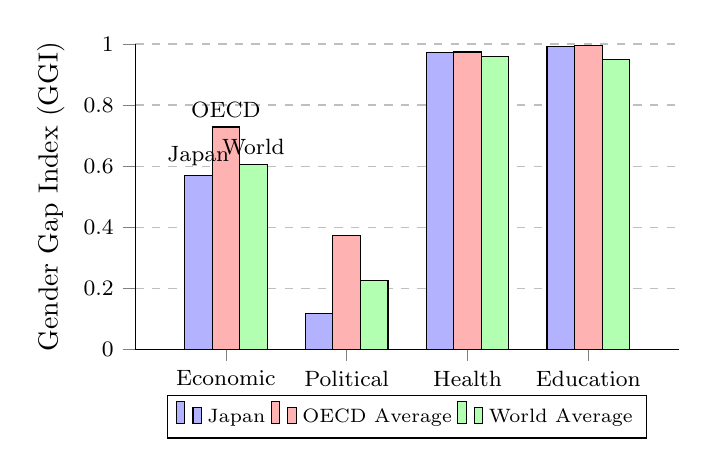
\begin{tikzpicture}
            \begin{axis}[
                ybar,
                bar width=0.35cm,
                width=0.7\textwidth,
                height=0.45\textwidth,
                enlarge x limits=0.25,
                symbolic x coords={Economic, Political, Health, Education},
                xtick=data,
                ymin=0, ymax=1,
                ylabel={Gender Gap Index (GGI)},
                ymajorgrids=true,
                grid style=dashed,
                enlarge y limits=0,
                axis x line*=bottom,
                axis y line*=left,
                tick align=outside,
                x tick label style={font=\footnotesize},
                y tick label style={font=\footnotesize},
                legend style={
                    at={(0.5,-0.15)},
                    anchor=north,
                    legend columns=3,
                    font=\scriptsize, % フォントサイズを一段階小さく
                },
            ]
            % Japan
            \addplot[
                pattern=north east lines,
                pattern color=blue,
                fill=blue!30,
                bar shift=-0.35cm, % 左にシフト
            ] coordinates {
                (Economic,0.568)
                (Political,0.118)
                (Health,0.973)
                (Education,0.993)
            };
            % OECD Average
            \addplot[
                pattern=crosshatch,
                pattern color=red,
                fill=red!30,
                bar shift=0cm, % 中央にシフトなし
            ] coordinates {
                (Economic,0.728)
                (Political,0.372)
                (Health,0.974)
                (Education,0.995)
            };
            % World Average
            \addplot[
                pattern=dots,
                pattern color=green,
                fill=green!30,
                bar shift=0.35cm, % 右にシフト
            ] coordinates {
                (Economic,0.605)
                (Political,0.225)
                (Health,0.960)
                (Education,0.949)
            };
            
            % ラベルの配置
            % 日本のEconomicバー
            \node[font=\footnotesize, above, xshift=-0.35cm] at (axis cs:Economic,0.568) {Japan};
            % OECD平均のEconomicバー
            \node[font=\footnotesize, above] at (axis cs:Economic,0.728) {OECD};
            % 世界平均のEconomicバー
            \node[font=\footnotesize, above, xshift=0.35cm] at (axis cs:Economic,0.605) {World};
            
            % 凡例の追加
            \legend{Japan, OECD Average, World Average}
            \end{axis}
        \end{tikzpicture}

    \vspace{0.1cm}
    \small Japan ranks 104th out of 146 countries in the 2024 Gender Gap Index. While scoring high in education and health, it lags significantly in economic participation and political empowerment. (Source: World Economic Forum, 2024)
    \end{figure}
\end{frame}

%%%%%%%%%%%%%%%%%%%%%%%%%%%%%%%%
%Income Bands by Gender
%%%%%%%%%%%%%%%%%%%%%%%%%%%%%%%%

\begin{frame}[label=income_band]
\frametitle{Income Bands by Gender: Pre- (2000-2010) vs Post-Disaster (2012-2018) Analysis (JGSS)}
\vspace{-0.4cm}
\returnbutton{income_band_main}{Return}
    \vspace{0.01cm}
    \begin{columns}[T]
        \begin{column}{0.7\textwidth}
            \raggedright
            \begin{table}
                \tiny
                \setlength{\tabcolsep}{1.2pt}
                \renewcommand{\arraystretch}{0.8}
                \begin{tabular}{lcccccccccccccc}
                    \toprule
                    & \multicolumn{14}{c}{Survey Year} \\
                    \cmidrule(lr){2-15}
                    Area & \quad \textcolor{blue}{2000} & \textcolor{blue}{2001} & \textcolor{blue}{2002} & \textcolor{blue}{2003} & \textcolor{blue}{2005} & \textcolor{blue}{2006} & \textcolor{blue}{2008} & \textcolor{blue}{2010} & \textcolor{red}{2012} & \textcolor{red}{2015} & \textcolor{red}{2016} & \textcolor{red}{2017} & \textcolor{red}{2018} & \quad Total\\
                    \midrule
                    Non-disaster area & \quad \textcolor{blue}{2,753} & \textcolor{blue}{2,664} & \textcolor{blue}{2,812} & \textcolor{blue}{3,462} & \textcolor{blue}{1,943} & \textcolor{blue}{4,084} & \textcolor{blue}{4,009} & \textcolor{blue}{4,772} & \textcolor{red}{4,461} & \textcolor{red}{1,976} & \textcolor{red}{922} & \textcolor{red}{714} & \textcolor{red}{1,810} & \quad 36,382 \\
                    Disaster-affected area & \quad \textcolor{blue}{140} & \textcolor{blue}{126} & \textcolor{blue}{141} & \textcolor{blue}{201} & \textcolor{blue}{80} & \textcolor{blue}{170} & \textcolor{blue}{211} & \textcolor{blue}{231} & \textcolor{red}{206} & \textcolor{red}{103} & \textcolor{red}{46} & \textcolor{red}{30} & \textcolor{red}{106} & \quad 1,791 \\
                    \midrule
                    Total & \quad \textcolor{blue}{2,893} & \textcolor{blue}{2,790} & \textcolor{blue}{2,953} & \textcolor{blue}{3,663} & \textcolor{blue}{2,023} & \textcolor{blue}{4,254} & \textcolor{blue}{4,220} & \textcolor{blue}{5,003} & \textcolor{red}{4,667} & \textcolor{red}{2,079} & \textcolor{red}{968} & \textcolor{red}{744} & \textcolor{red}{1,916} & \quad 38,173 \\
                    \bottomrule
                \end{tabular}
            \end{table}
            \vspace{-0.63cm}
            \begin{figure}
                \includegraphics[width=0.65\textwidth]{Kernel density graphs of respondent’s annual income from main job.png}
                \vspace{-0.15cm}
                \captionsetup{font=tiny}
                \caption{Kernel Density of Respondent's Annual Income from Main Job (Income Bands, N=20,119)}
                \label{fig:Kernel_density}
            \end{figure}
        \end{column}
        \begin{column}{0.3\textwidth}
    \vspace{3.0cm}
    \hspace{-1.1cm}
    \fbox{
        \parbox{\linewidth}{
            \small Only the 'Women in affected prefectures' group experienced a rightward shift (increase) in average income bands when comparing pre- and post-disaster periods.
        }
    }
\end{column}
    \end{columns}
\end{frame}

%%%%%%%%%%%%%%%%%%%%%



\begin{frame}

Basic DID analysis. (Population Census)

\begin{table}[htbp]
\centering
\caption{OLS Estimates of Disaster Impact on Regular Worker Status}

\scalefont{0.7}
\begin{tabular}{@{}l*{6}{c}@{}}
          &\multicolumn{3}{c}{Male}                                &\multicolumn{3}{c}{Female}                              \\\cmidrule(lr){2-4}\cmidrule(lr){5-7}
          &\multicolumn{1}{c}{(1)}&\multicolumn{1}{c}{(2)}&\multicolumn{1}{c}{(3)}&\multicolumn{1}{c}{(4)}&\multicolumn{1}{c}{(5)}&\multicolumn{1}{c}{(6)}\\
          &\multicolumn{1}{c}{Basic}&\multicolumn{1}{c}{Age, Married}&\multicolumn{1}{c}{Full}&\multicolumn{1}{c}{Basic}&\multicolumn{1}{c}{Age, Married}&\multicolumn{1}{c}{Full}\\
\toprule
Disaster Impact (DID)&   -0.015\sym{***}&   -0.010\sym{***}&   -0.003\sym{**} &    0.004\sym{**} &    0.004\sym{***}&    0.003\sym{**} \\
          &  (0.003)         &  (0.003)         &  (0.001)         &  (0.002)         &  (0.001)         &  (0.001)         \\
\addlinespace
Post-Disaster Period&   -0.006\sym{**} &   -0.000         &   -0.004\sym{***}&    0.004\sym{**} &    0.009\sym{***}&    0.001         \\
          &  (0.003)         &  (0.003)         &  (0.001)         &  (0.002)         &  (0.001)         &  (0.001)         \\
\addlinespace
Married   &                  &    0.161\sym{***}&    0.119\sym{***}&                  &   -0.175\sym{***}&   -0.168\sym{***}\\
          &                  &  (0.005)         &  (0.002)         &                  &  (0.004)         &  (0.004)         \\
\midrule
Age       &       No         &      Yes         &      Yes         &       No         &      Yes         &      Yes         \\
Residence Duration&       No         &       No         &      Yes         &       No         &       No         &      Yes         \\
Industry  &       No         &       No         &      Yes         &       No         &       No         &      Yes         \\
$\textit{N}$&  659,324         &  659,324         &  659,324         &  505,463         &  505,463         &  505,463         \\
$\textit{R}^2$&    0.006         &    0.106         &    0.257         &    0.004         &    0.060         &    0.155         \\
\bottomrule
\end{tabular}
\\\multicolumn{7}{@{}p{\linewidth}}{\footnotesize Standard errors clustered at prefecture level in parentheses}\\
\multicolumn{7}{@{}p{\linewidth}}{\footnotesize $*p<0.1$, $**p<0.05$, $***p<0.01$}\\

\label{table:DID_OLS}

\end{table}

\end{frame}

%%%%%%%%%%%%%%%%%%%%%%%%%%%%%%%%

%%%%%%%%%%%%%%%%%%%%%%%%%%%%%%%%%%%


\begin{frame}

Basic DID analysis. (Population Census)


\begin{table}[htbp]
\centering
\caption{OLS Estimates of Disaster Impact on Employment Status}
\scalefont{0.61}

\begin{tabular}{@{}l*{6}{c}@{}}
          &\multicolumn{3}{c}{Male}                                &\multicolumn{3}{c}{Female}                              \\\cmidrule(lr){2-4}\cmidrule(lr){5-7}
          &\multicolumn{1}{c}{(1)}&\multicolumn{1}{c}{(2)}&\multicolumn{1}{c}{(3)}&\multicolumn{1}{c}{(4)}&\multicolumn{1}{c}{(5)}&\multicolumn{1}{c}{(6)}\\
          &\multicolumn{1}{c}{Basic}&\multicolumn{1}{c}{Age, Married}&\multicolumn{1}{c}{Full}&\multicolumn{1}{c}{Basic}&\multicolumn{1}{c}{Age, Married}&\multicolumn{1}{c}{Full}\\
\toprule
Disaster Impact (DID)&    0.033\sym{***}&    0.032\sym{***}&    0.032\sym{***}&    0.009\sym{***}&    0.004         &    0.006\sym{***}\\
          &  (0.004)         &  (0.004)         &  (0.002)         &  (0.002)         &  (0.003)         &  (0.002)         \\
\addlinespace
Post-Disaster Period&   -0.016\sym{***}&    0.006         &    0.015\sym{***}&    0.007\sym{***}&    0.024\sym{***}&    0.030\sym{***}\\
          &  (0.004)         &  (0.005)         &  (0.003)         &  (0.002)         &  (0.003)         &  (0.002)         \\
\addlinespace
Married   &                  &    0.199\sym{***}&    0.111\sym{***}&                  &   -0.081\sym{***}&   -0.056\sym{***}\\
          &                  &  (0.006)         &  (0.003)         &                  &  (0.005)         &  (0.004)         \\
\midrule
Age       &       No         &      Yes         &      Yes         &       No         &      Yes         &      Yes         \\
Residence Duration&       No         &       No         &      Yes         &       No         &       No         &      Yes         \\
Relationship with Head&       No         &       No         &      Yes         &       No         &       No         &      Yes         \\
Residence Type&       No         &       No         &      Yes         &       No         &       No         &      Yes         \\
Household Size&       No         &       No         &      Yes         &       No         &       No         &      Yes         \\
$\textit{N}$&  1041395         &  1041395         &  1041395         &  1122154         &  1122154         &  1122154         \\
$\textit{R}^2$&    0.004         &    0.345         &    0.423         &    0.002         &    0.252         &    0.291         \\
\bottomrule
\end{tabular}
\\\multicolumn{7}{@{}p{\linewidth}}{\footnotesize Standard errors clustered at prefecture level in parentheses}\\
\multicolumn{7}{@{}p{\linewidth}}{\footnotesize $*p<0.1$, $**p<0.05$, $***p<0.01$}\\

\label{tab:did_employment_status}

\end{table}

\end{frame}

%%%%%%%%%%%%%%%%%%%%%%%%%%%%%%%%
%%%%%%%%%%%%%%%%%%%%%%%%%%%%%%%%%%%

\begin{frame}


\begin{table}[htbp]
\centering
\caption{DID Estimates of Disaster Impact on Different Employment Types}

\scalefont{0.61}

\begin{tabular}{@{}l*{6}{c}@{}}
          &\multicolumn{1}{c}{Regular Employee}&\multicolumn{1}{c}{Temp Agency Worker}&\multicolumn{1}{c}{Part-time Worker}&\multicolumn{1}{c}{Executive}&\multicolumn{1}{c}{Self-employed}&\multicolumn{1}{c}{Family Worker}\\\cmidrule(lr){2-2}\cmidrule(lr){3-3}\cmidrule(lr){4-4}\cmidrule(lr){5-5}\cmidrule(lr){6-6}\cmidrule(lr){7-7}
          &\multicolumn{1}{c}{(1)}         &\multicolumn{1}{c}{(2)}         &\multicolumn{1}{c}{(3)}         &\multicolumn{1}{c}{(4)}         &\multicolumn{1}{c}{(5)}         &\multicolumn{1}{c}{(6)}         \\
\toprule
Disaster Impact (DID)&    0.008\sym{***}&   -0.001\sym{***}&   -0.001         &   -0.001\sym{**} &   -0.005\sym{***}&   -0.001\sym{***}\\
          &  (0.001)         &  (0.000)         &  (0.001)         &  (0.000)         &  (0.000)         &  (0.000)         \\
\addlinespace
Post-Disaster Period&    0.005\sym{***}&    0.001\sym{***}&    0.004\sym{***}&   -0.003\sym{***}&   -0.005\sym{***}&   -0.002\sym{***}\\
          &  (0.001)         &  (0.000)         &  (0.001)         &  (0.000)         &  (0.000)         &  (0.000)         \\
\addlinespace
Fukushima &    0.009\sym{***}&    0.002\sym{***}&   -0.023\sym{***}&   -0.001\sym{***}&    0.008\sym{***}&    0.005\sym{***}\\
          &  (0.001)         &  (0.000)         &  (0.001)         &  (0.000)         &  (0.000)         &  (0.000)         \\
\addlinespace
Married   &   -0.016\sym{***}&   -0.011\sym{***}&   -0.001         &    0.015\sym{***}&    0.002\sym{***}&    0.011\sym{***}\\
          &  (0.002)         &  (0.001)         &  (0.002)         &  (0.000)         &  (0.001)         &  (0.000)         \\
\midrule
$\textit{N}$&1,301,352         &1,301,352         &1,301,352         &1,301,352         &1,301,352         &1,301,352         \\
$\textit{R}^2$&    0.485         &    0.031         &    0.219         &    0.066         &    0.191         &    0.168         \\
Control Mean&    0.245         &    0.010         &    0.114         &    0.024         &    0.049         &    0.023         \\
\bottomrule
\end{tabular}
\\\multicolumn{7}{@{}p{\linewidth}}{\footnotesize Standard errors clustered at prefecture level in parentheses}\\
\multicolumn{7}{@{}p{\linewidth}}{\footnotesize $*p<0.1$, $**p<0.05$, $***p<0.01$}\\


\end{table}

\end{frame}

%%%%%%%%%%%%%%%%%%%%%%%%%%%%%%%%
%%%%%%%%%%%%%%%%%%%%%%%%%%%%%%%%
\begin{frame}{Methodology and Empirical Strategy: TWEF Event Study with a triple difference estimator}
    \begin{itemize}
    \item Two-Way Fixed Effects (TWFE) Event Study approach with a triple difference estimator, incorporating gender differences and including both individual fixed effects and time fixed effects:

\begin{equation}
Y_{ipgt} = \beta_i + \eta_t + \sum_{l \in L} (\delta_l\ + \gamma_l \cdot Female_i) \cdot 1[t-s = l] +  \mathbf \gamma {X}_{ipgt}+\epsilon_{ipgt}
\end{equation}
\end{itemize}

\end{frame}
%%%%%%%%%%%%%%%%%%%%%%%%%%%%%%%%

%%%%%%%%%%%%%%%%%%%%%%%%%%%%%%%%

\begin{frame}

Basic DID analysis. (JHPS-CPS)

\begin{table}[htbp]
\centering
\caption{DID Estimates of Disaster Impact on Monthly Income}

\scalefont{0.61}
\begin{tabular}{@{}l*{6}{c}@{}}
          &\multicolumn{3}{c}{Male}                                &\multicolumn{3}{c}{Female}                              \\\cmidrule(lr){2-4}\cmidrule(lr){5-7}
          &\multicolumn{1}{c}{(1)}&\multicolumn{1}{c}{(2)}&\multicolumn{1}{c}{(3)}&\multicolumn{1}{c}{(4)}&\multicolumn{1}{c}{(5)}&\multicolumn{1}{c}{(6)}\\
          &\multicolumn{1}{c}{Basic}&\multicolumn{1}{c}{Education}&\multicolumn{1}{c}{Edu+Occ}&\multicolumn{1}{c}{Basic}&\multicolumn{1}{c}{Education}&\multicolumn{1}{c}{Edu+Occ}\\
\toprule
Disaster Impact (DID)&   -0.841         &   -0.835         &   -1.444         &    0.633         &    0.575         &    1.114\sym{***}\\
          &  (1.151)         &  (1.132)         &  (1.204)         &  (0.521)         &  (0.493)         &  (0.238)         \\
\addlinespace
Post-Disaster Period&   -1.083\sym{***}&   -1.055\sym{***}&   -0.844\sym{**} &    0.148         &    0.159         &    0.033         \\
          &  (0.315)         &  (0.317)         &  (0.325)         &  (0.263)         &  (0.265)         &  (0.282)         \\
\addlinespace
Age       &    2.875\sym{***}&    2.842\sym{***}&    2.397\sym{***}&    1.414\sym{***}&    1.413\sym{***}&    1.030\sym{***}\\
          &  (0.209)         &  (0.215)         &  (0.196)         &  (0.189)         &  (0.180)         &  (0.167)         \\
\addlinespace
Age Squared&   -0.029\sym{***}&   -0.029\sym{***}&   -0.024\sym{***}&   -0.013\sym{***}&   -0.013\sym{***}&   -0.009\sym{***}\\
          &  (0.002)         &  (0.002)         &  (0.002)         &  (0.002)         &  (0.002)         &  (0.001)         \\
\midrule
Education &       No         &      Yes         &      Yes         &       No         &      Yes         &      Yes         \\
Occupation&       No         &       No         &      Yes         &       No         &       No         &      Yes         \\
$\textit{N}$&   11,419         &   11,313         &   10,986         &   10,493         &   10,407         &   10,055         \\
$\textit{Adjusted R}^2$&    0.759         &    0.760         &    0.772         &    0.620         &    0.620         &    0.635         \\
\bottomrule
\end{tabular}
\\\multicolumn{7}{@{}p{\linewidth}}{\footnotesize Standard errors clustered at prefecture level in parentheses}\\
\multicolumn{7}{@{}p{\linewidth}}{\footnotesize $*p<0.1$, $**p<0.05$, $***p<0.01$}\\


\label{table:basic_DID_Monthly_income}

\end{table}

\end{frame}

%%%%%%%%%%%%%%%%%%%%%%%%%%%%%%%%

\begin{frame}


Results of the TWFE Event Study

%******************************************
%* TWFE Event Study: Impact of Disaster on Monthly Income: Female
%******************************************

\begin{table}[htbp]
\centering
\caption{Effects of Disaster on Monthly Income of Females in Disaster-Affected Prefectures}

\scalefont{0.315}

\begin{tabular}{@{\extracolsep{5pt}}lccccc}
            &\multicolumn{1}{c}{(1)}&\multicolumn{1}{c}{(2)}&\multicolumn{1}{c}{(3)}&\multicolumn{1}{c}{(4)}&\multicolumn{1}{c}{(5)}\\
            &\multicolumn{1}{c}{OLS Basic Model}&\multicolumn{1}{c}{OLS Age Control}&\multicolumn{1}{c}{OLS Full Model}&\multicolumn{1}{c}{IPW ATE}&\multicolumn{1}{c}{IPW ATT}\\
\midrule
2 years before (Year 2009)&       1.805         &       1.498         &       0.529         &       1.261         &       1.359         \\
            &     (1.547)         &     (1.523)         &     (2.042)         &     (1.929)         &     (1.955)         \\
\addlinespace
1 year before (Year 2010)&       0.085         &      -0.137         &      -0.797         &      -0.866         &      -0.731         \\
            &     (1.220)         &     (1.196)         &     (1.253)         &     (0.956)         &     (1.248)         \\
\addlinespace
Baseline, 2 months before (Year 2011)&       0.000         &       0.000         &       0.000         &       0.000         &       0.000         \\
            &         (.)         &         (.)         &         (.)         &         (.)         &         (.)         \\
\addlinespace
1 year after (Year 2012)&       1.180         &       1.242         &       2.093\sym{*}  &       2.305\sym{*}  &       2.476\sym{*}  \\
            &     (1.300)         &     (1.319)         &     (1.209)         &     (1.307)         &     (1.316)         \\
\addlinespace
2 years after (Year 2013)&       0.497         &       0.804         &       1.470         &       1.665         &       1.999         \\
            &     (2.047)         &     (2.000)         &     (1.875)         &     (2.242)         &     (2.230)         \\
\addlinespace
5 years after (Year 2016)&       3.823         &       5.023\sym{*}  &       5.907\sym{**} &       5.803\sym{**} &       5.900\sym{**} \\
            &     (2.726)         &     (2.930)         &     (2.367)         &     (2.554)         &     (2.456)         \\
\addlinespace
6 years after (Year 2017)&      -0.320         &       0.909         &       1.391         &       0.641         &       1.663         \\
            &     (3.121)         &     (3.365)         &     (3.649)         &     (4.624)         &     (3.967)         \\
\addlinespace
7 years after (Year 2018)&       2.888         &       4.448\sym{*}  &       4.074\sym{*}  &       3.771\sym{*}  &       3.754         \\
            &     (2.330)         &     (2.376)         &     (2.070)         &     (2.159)         &     (2.484)         \\
\addlinespace
Age         &                     &       2.347\sym{***}&       1.976\sym{***}&       1.238\sym{*}  &       1.461\sym{*}  \\
            &                     &     (0.324)         &     (0.281)         &     (0.651)         &     (0.779)         \\
\addlinespace
Age Squared &                     &      -0.022\sym{***}&      -0.018\sym{***}&      -0.016\sym{***}&      -0.016\sym{***}\\
            &                     &     (0.001)         &     (0.001)         &     (0.002)         &     (0.003)         \\
\midrule
Education   &          No         &          No         &         Yes         &         Yes         &         Yes         \\
Occupation  &          No         &          No         &         Yes         &         Yes         &         Yes         \\
$\textit{N}$&      21,912         &      21,912         &      21,041         &      20,569         &      20,569         \\
$\textit{Adjusted R}^2$&       0.776         &       0.783         &       0.795         &       0.762         &       0.739         \\
\bottomrule
\multicolumn{6}{l}{\footnotesize Standard errors in parentheses}\\
\multicolumn{6}{l}{\footnotesize \sym{*} \(p<0.1\), \sym{**} \(p<0.05\), \sym{***} \(p<0.01\)}\\

\end{tabular}

\label{table:Monthly_Income}

\end{table}

\end{frame}

%%%%%%%%%%%%%%%%%%%%%%%%%%%%%%%%

\begin{frame}

\begin{figure}[h!]
    \centering
    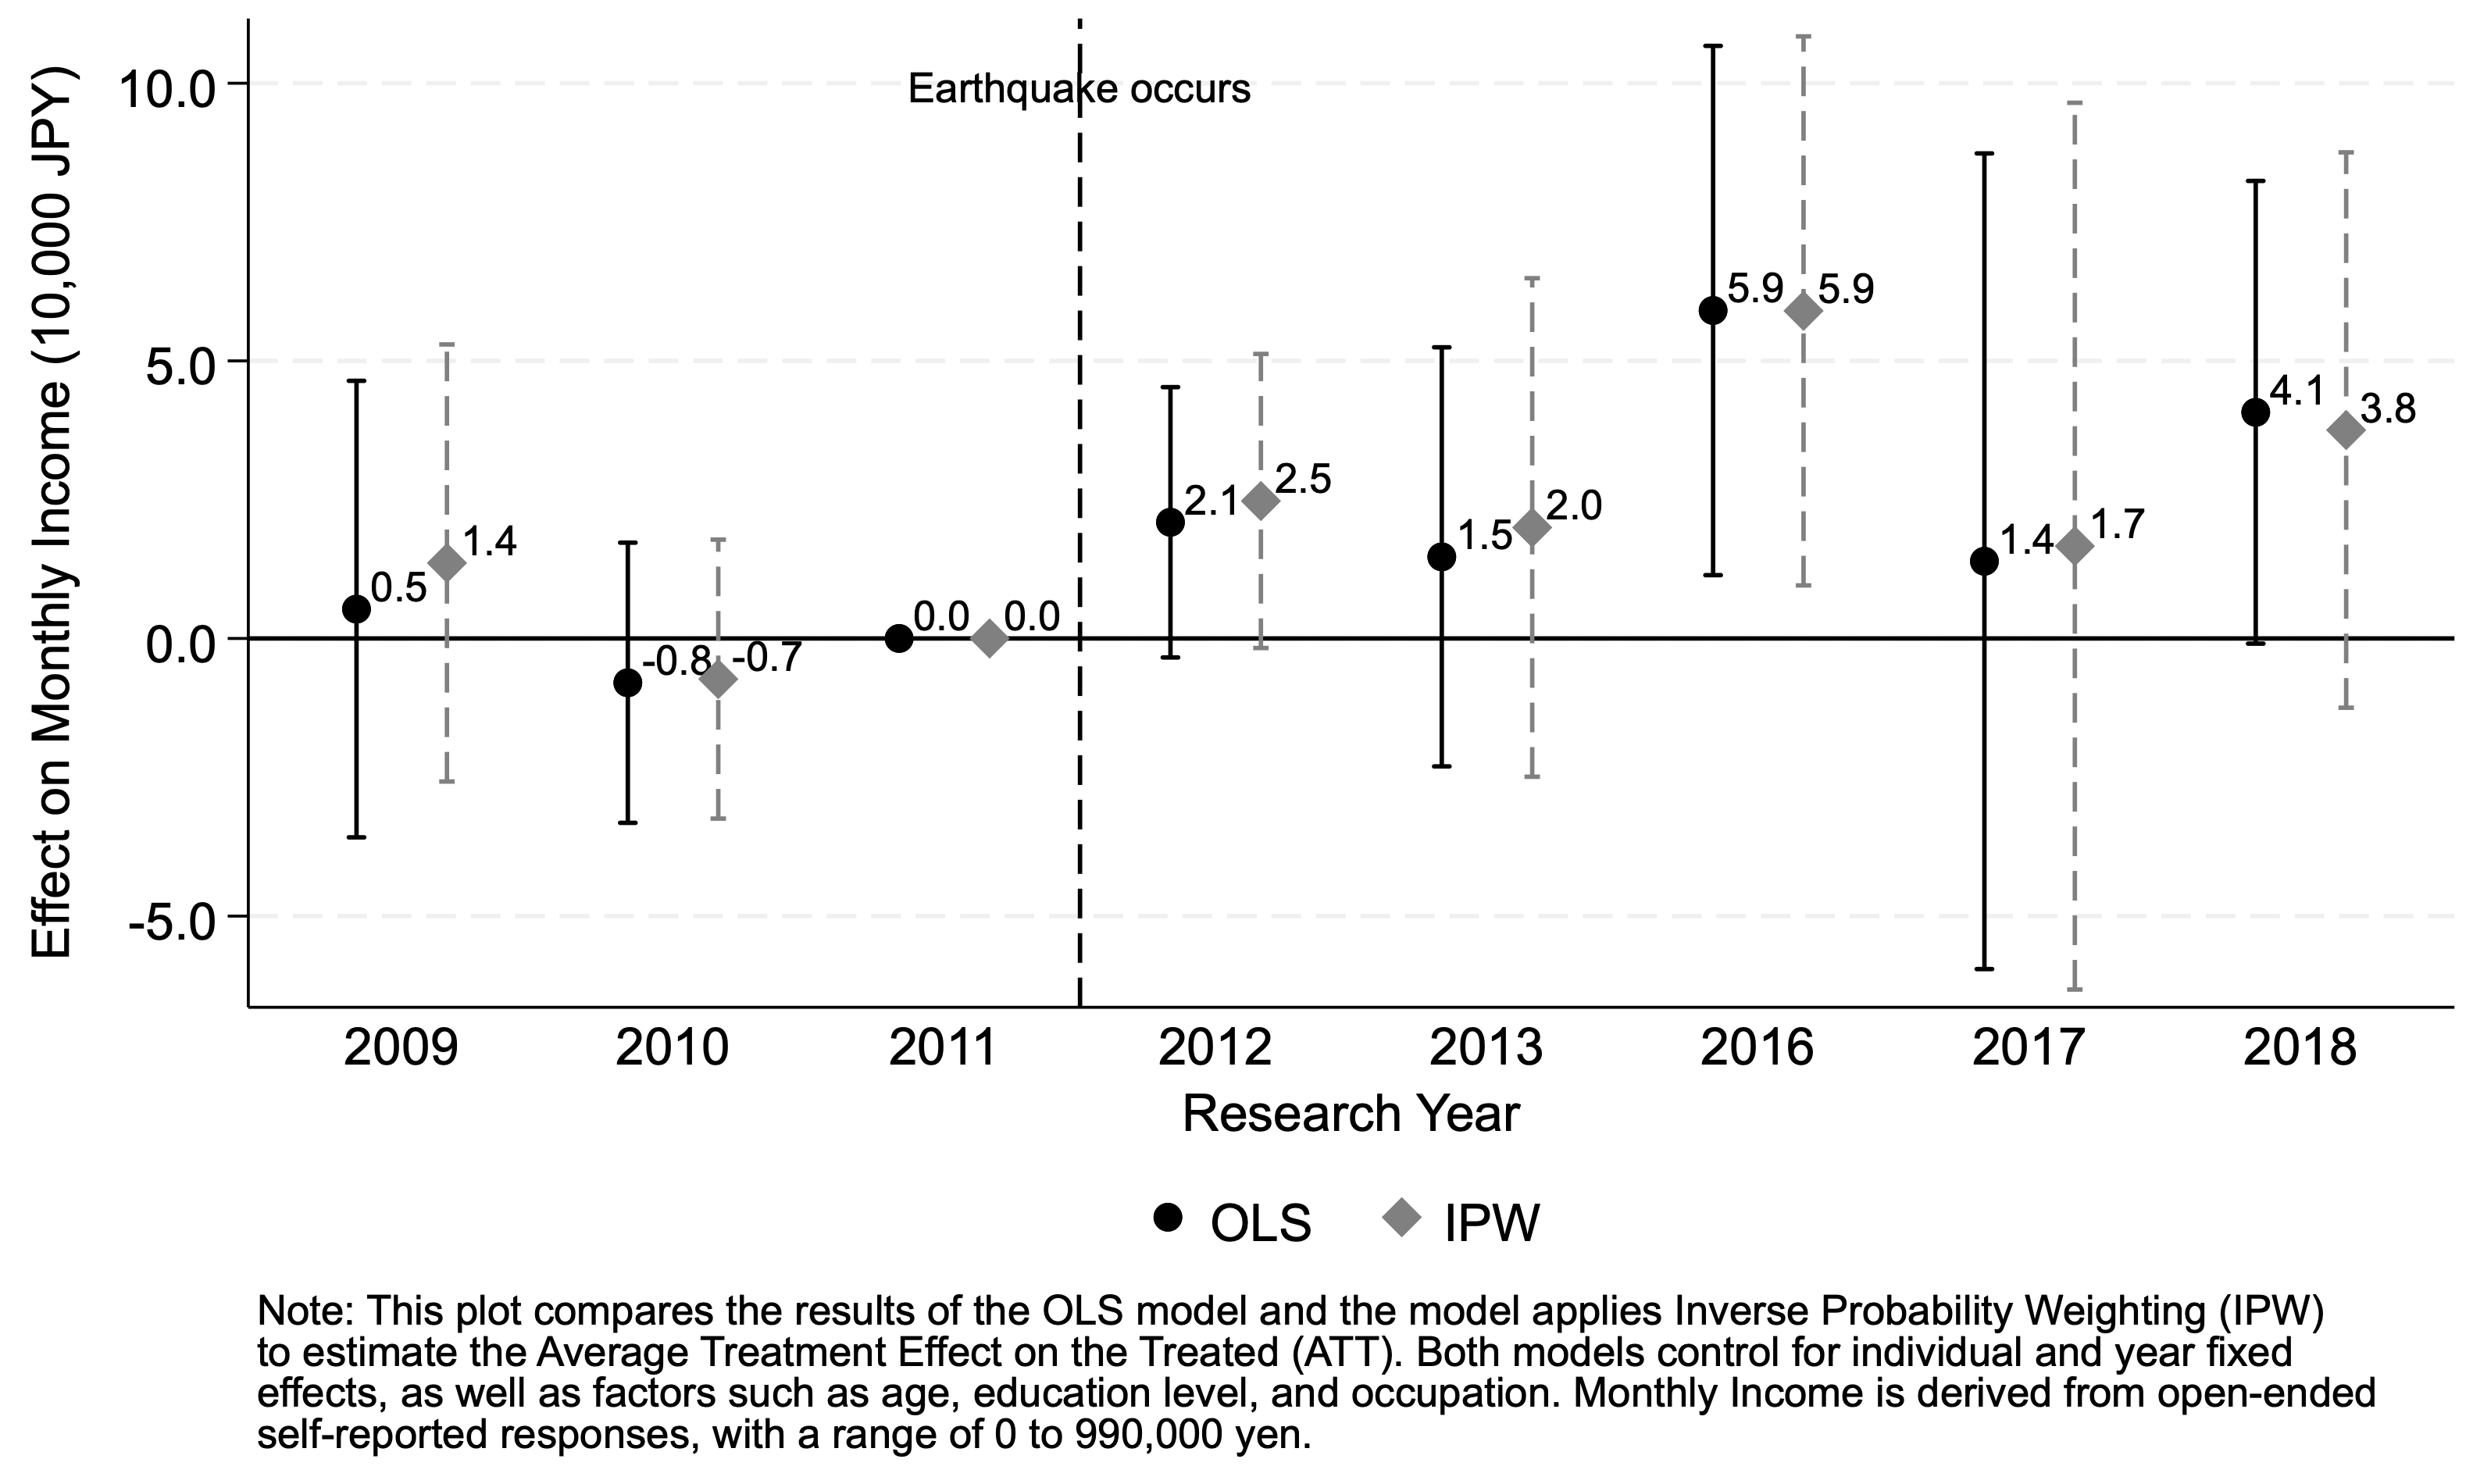
\includegraphics[width=0.70\textwidth]{monthly_income_comparison.png}  % 幅を本文の80%に設定
    \caption{TWFE Event Study: Effects on Females in Disaster-Affected Prefectures}

\end{figure}

\end{frame}

%%%%%%%%%%%%%%%%%%%%%%%%%%%%%%%%


%---------------------------------------
% Slide: Fishery in Fukushima
%---------------------------------------


\begin{frame}[label=image]
\frametitle{Types of Employment in Fukushima's Fisheries}

\vspace{0.2cm}

\returnbutton{conclusion}{Return}


    \vspace{-0.2cm}
  \begin{figure}
    \centering
    \includegraphics[width=0.93\textwidth]{Fishery-1.0.pdf}

  \end{figure}
\end{frame}


%%%%%%%%%%%%%%%%%%%%%%%%%%%%%%%%
% Labour Force Participation Rates
%%%%%%%%%%%%%%%%%%%%%%%%%%%%%%%%


\begin{frame}[label=LFP]
    \frametitle{Labor Force Participation Rates by Age and Gender - Fukushima Pref}

    \vspace{0.25cm}

    \returnbutton{conclusion}{Return}

    \vspace{-0.4cm}

    \begin{figure}
        \centering

        \begin{subfigure}{\textwidth}
            \centering
            \begin{minipage}{0.48\textwidth}
                \centering
                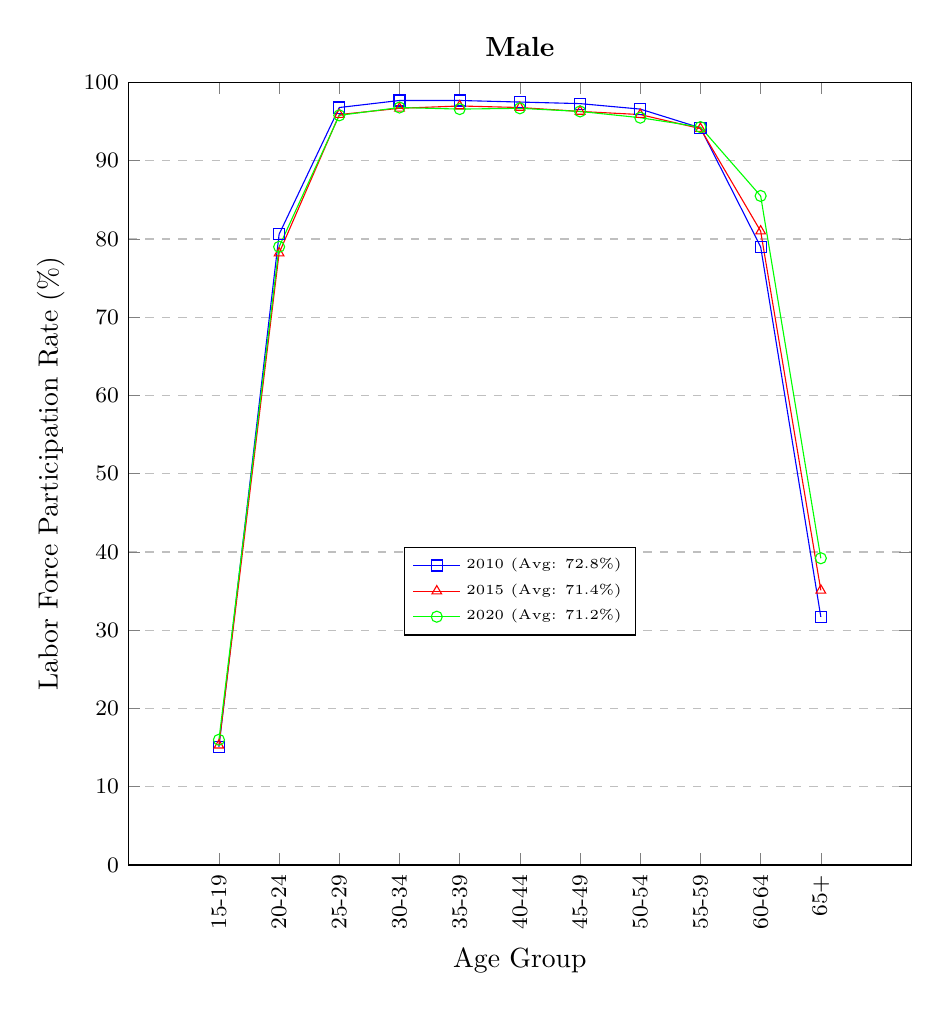
\begin{tikzpicture}
                \begin{axis}[
                    title={\textbf{Male}},
                    xlabel={Age Group},
                    ylabel={Labor Force Participation Rate (\%)},
                    xmin=0, xmax=12,
                    ymin=0, ymax=100,
                    xtick={1,2,3,4,5,6,7,8,9,10,11},
                    xticklabels={15-19,20-24,25-29,30-34,35-39,40-44,45-49,50-54,55-59,60-64,65+},
                    x tick label style={rotate=90,anchor=east,font=\footnotesize},
                    y tick label style={font=\footnotesize},
                    legend style={font=\tiny, at={(0.5,0.35)}, anchor=center, legend columns=1},
                    ymajorgrids=true,
                    grid style=dashed,
                    enlarge x limits={abs=0.5},
                    width=0.95\linewidth,
                    height=0.95\linewidth,
                ]

                \addplot[color=blue, mark=square] coordinates {
                    (1,15.1)(2,80.6)(3,96.8)(4,97.7)(5,97.7)(6,97.5)(7,97.3)(8,96.6)(9,94.2)(10,79.0)(11,31.7)
                };

                \addplot[color=red, mark=triangle] coordinates {
                    (1,15.3)(2,78.2)(3,95.9)(4,96.7)(5,97.0)(6,96.8)(7,96.3)(8,95.9)(9,94.1)(10,81.0)(11,35.1)
                };

                \addplot[color=green, mark=o] coordinates {
                    (1,16.0)(2,79.0)(3,95.8)(4,96.8)(5,96.6)(6,96.7)(7,96.3)(8,95.5)(9,94.3)(10,85.5)(11,39.2)
                };

                \legend{
                    2010 (Avg: 72.8\%),
                    2015 (Avg: 71.4\%),
                    2020 (Avg: 71.2\%)
                }
                \end{axis}
                \end{tikzpicture}
            \end{minipage}
            \hfill
            \begin{minipage}{0.48\textwidth}
                \centering
                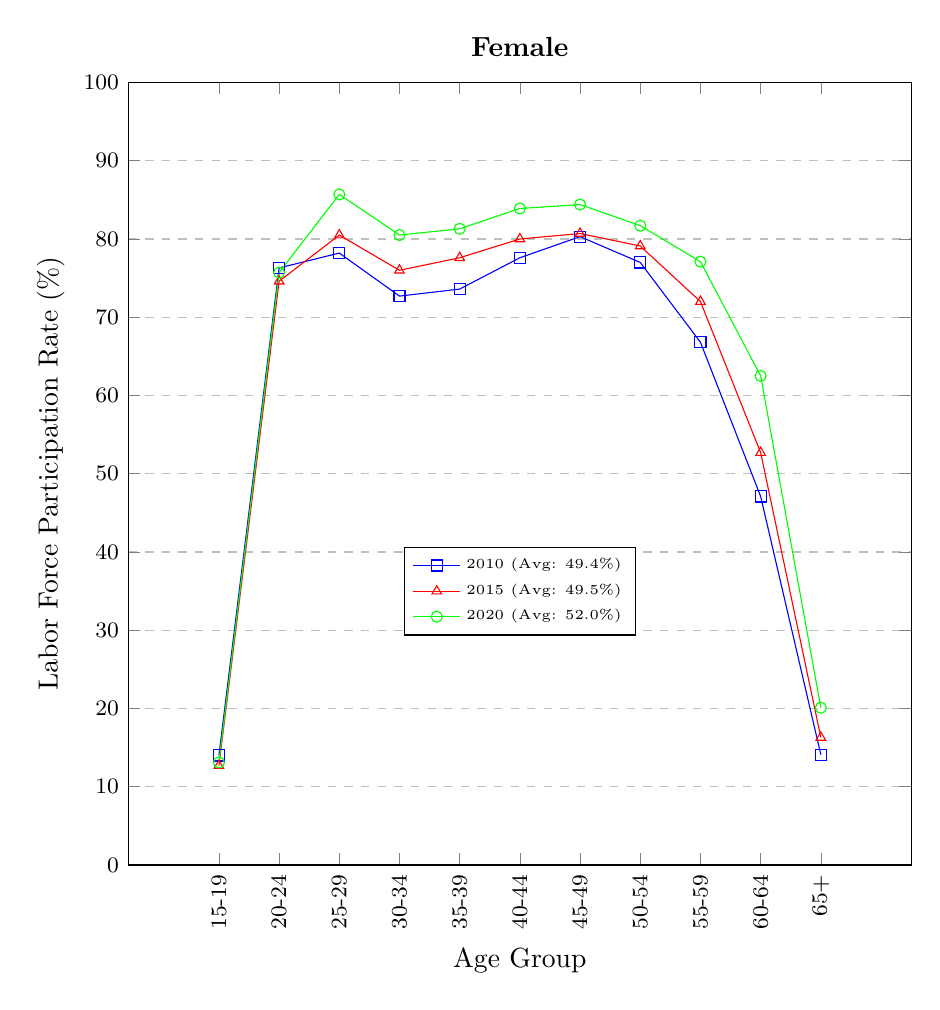
\begin{tikzpicture}
                \begin{axis}[
                    title={\textbf{Female}},
                    xlabel={Age Group},
                    ylabel={Labor Force Participation Rate (\%)},
                    xmin=0, xmax=12,
                    ymin=0, ymax=100,
                    xtick={1,2,3,4,5,6,7,8,9,10,11},
                    xticklabels={15-19,20-24,25-29,30-34,35-39,40-44,45-49,50-54,55-59,60-64,65+},
                    x tick label style={rotate=90,anchor=east,font=\footnotesize},
                    y tick label style={font=\footnotesize},
                    legend style={font=\tiny, at={(0.5,0.35)}, anchor=center, legend columns=1},
                    ymajorgrids=true,
                    grid style=dashed,
                    enlarge x limits={abs=0.5},
                    width=0.95\linewidth,
                    height=0.95\linewidth,
                ]

                \addplot[color=blue, mark=square] coordinates {
                    (1,14.0)(2,76.3)(3,78.2)(4,72.7)(5,73.6)(6,77.6)(7,80.3)(8,77.0)(9,66.8)(10,47.1)(11,14.1)
                };

                \addplot[color=red, mark=triangle] coordinates {
                    (1,12.7)(2,74.6)(3,80.5)(4,76.0)(5,77.6)(6,80.0)(7,80.7)(8,79.1)(9,72.0)(10,52.7)(11,16.3)
                };

                \addplot[color=green, mark=o] coordinates {
                    (1,13.1)(2,75.7)(3,85.7)(4,80.5)(5,81.3)(6,83.9)(7,84.4)(8,81.7)(9,77.1)(10,62.5)(11,20.1)
                };

                \legend{
                    2010 (Avg: 49.4\%),
                    2015 (Avg: 49.5\%),
                    2020 (Avg: 52.0\%)
                }
                \end{axis}
                \end{tikzpicture}
            \end{minipage}
        \end{subfigure}

    \end{figure}

\end{frame}

%%%%%%%%%%%%%%%%%%%%%%%%%%%%%%%%%%%%%%%%%

%\section{References}

\begin{frame}[allowframebreaks]
    \frametitle{References}
    \small % 文字サイズを小さくして、より多くの参考文献を1ページに収める
    \bibliographystyle{apacite} % APAスタイルを使用
    \bibliography{references}
    % \nocite{*} コマンドを削除
\end{frame}


%%%%%%%%%%%%%%%%%%%%%%%%%%%%%%%%






\end{document}